\documentclass[a4paper,adobefonts,11pt,UTF8]{book}

%type chinese characters
\usepackage{ctex}

%Bibliography
\usepackage{chapterbib}
\usepackage[sectionbib,square,super,sort&compress]{natbib}


%generate index of book
\usepackage{makeidx}

%modify the headheight at least 13.5pt
\usepackage[headheight=13.6pt]{geometry}

%%\usepackage{caption}
%%\DeclareCaptionType [fileext=loe]{example}[Example][List of Examples]
%%
%%\usepackage{subfig}                 % put before fvrb-ex
%%\newsubfloat[position=bottom,listofformat=subsimple]{example}

%
\usepackage{fontspec}

%unicode
\usepackage{xunicode}

%
\usepackage{xltxtra}

%mathematics package
\usepackage{amsmath}

%mathematics symbols
\usepackage{amssymb}

%origin print package
\usepackage{verbatim}

%draw graphics use tikz and so on.
\usepackage{graphicx}

%set graphics path which used in the book.
\graphicspath{{../img/}}

%colorful table
\usepackage{colortbl}

%set color use origin name directly.
\usepackage[svgnames,table]{xcolor}

%
\usepackage[figuresright]{rotating}

% generate longtable which could across pages.
\usepackage{longtable}

%
\usepackage{multirow}

%
\usepackage{adjustbox}


%
\newcommand\mgape[1]{\gape{$\vcenter{\hbox{#1}}$}}

%
\usepackage{array}

%
\usepackage{makecell}

%
\usepackage{ulem}

%
\usepackage{color}

% draw graphics use tikz package
\usepackage{tikz}

%
\usepackage{listings}
\lstset{
  basicstyle=\ttfamily,
  showstringspaces=false,
  commentstyle=\color{red},
  keywordstyle=\color{blue},
  columns=flexible,
  backgroundcolor=\color{lightgray},
  extendedchars=true,
  basicstyle=\footnotesize\ttfamily,
  showstringspaces=false,
  showspaces=false,
  %numbers=left,
  %numberstyle=\footnotesize,
  %numbersep=9pt,
  tabsize=2,
  breaklines=true,
  showtabs=false,
  captionpos=b
}

%
\usepackage{bashful}

%set book information including bookmarksnumbered,pdfencoding,
%pdfauthor,pdfpagelayout,breaklinks,colorlinks,linkcolor,
%urlcolor,and so on.
\usepackage[bookmarksnumbered,pdfencoding=auto,pdfauthor={穷屌丝联盟},pdfpagelayout=TwoPageRight,breaklinks,colorlinks,linkcolor=RoyalBlue,urlcolor=blue,colorlinks=true]{hyperref}

%add more list types.
\usepackage{paralist}

%set page styles
\usepackage{fancyhdr}

\pagestyle{fancy}
\fancyhf{}
\fancyhead[LE,RO]{\thepage}
\fancyhead[RE]{\leftmark}
\fancyhead[RO]{\rightmark}
\fancypagestyle{plain}{
  \fancyhf{}
  \renewcommand{\headrulewidth}{0pt}
}


%titlepage \titleGM
\newcommand*{\plogo}{\fbox{$\mathcal{PL}$}} % Generic publisher logo
%--------------------------------------------------------------------
% TITLE PAGE
%--------------------------------------------------------------------

\newcommand*{\titleGM}{\begingroup % Create the command for including the title page in the document
\hbox{ % Horizontal box
\hspace*{0.2\textwidth} % Whitespace to the left of the title page
\rule{1pt}{\textheight} % Vertical line
\hspace*{0.05\textwidth} % Whitespace between the vertical line and title page text
\parbox[b]{0.75\textwidth}{ % Paragraph box which restricts text to less than the width of the page
{\noindent\Huge\bfseries Notes Collection of \\[0.5\baselineskip] VUE}\\[2\baselineskip] % Title
{\large \textit{VUE}}\\[4\baselineskip] % Tagline or further description
{\Large \textsc{theqiong.com}} % Author name

\vspace{0.5\textheight} % Whitespace between the title block and the publisher
{\noindent 穷屌丝联盟}\\[\baselineskip] % Publisher and logo
}}
\endgroup}
%


%lstlisting[language=JavsScript]
% Taken from Lena Herrmann at 
% http://lenaherrmann.net/2010/05/20/javascript-syntax-highlighting-in-the-latex-listings-package
\definecolor{lightgray}{rgb}{.9,.9,.9}
\definecolor{darkgray}{rgb}{.4,.4,.4}
\definecolor{purple}{rgb}{0.65,0.12,0.82}

%lstlisting package -----------
% JavaScript
%------------------------------
\lstdefinelanguage{JavaScript}
{
  keywords={typeof,new,ture,false,catch,function,return,null,switch,var,if,in,while,do,else,case,break},
  keywordstyle=\color{blue}\bfseries,
  ndkeywords={class,export,boolean,throw,implements,import,this},
  ndkeywordstyle=\color{darkgray}\bfseries,
  identifierstyle=\color{black},
  sensitive=false,
  comment=[l]{//},
  %morecomments[s]{/*}{*/},
  commentstyle=\color{purple}\ttfamily,
  stringstyle=\color{red}\ttfamily,
  morestring=[b]',
  morestring=[b]"
}

\lstdefinelanguage{Scheme}
{morekeywords={,lambda, cond, case, display, let, import, quote, quasiquote, unquote,
define, begin, newline, if, list, apply, null?, car, cdr, or, not, and, for-each, 
make-vector, vector-length, vector-ref, vector-set!, eqv?, eq?, equal?, else, set!, 
define-record-type, fields, mutable, immutable, assert, parent, with-exception-handler, }
sensitive=false,
morecomment=[l]{;},
morecomment=[s]{/*}{*/},
morestring=[b]",
}

\lstdefinelanguage{CSS}{
  morekeywords={accelerator,azimuth,background,background-attachment,
    background-color,background-image,background-position,
    background-position-x,background-position-y,background-repeat,
    behavior,border,border-bottom,border-bottom-color,
    border-bottom-style,border-bottom-width,border-collapse,
    border-color,border-left,border-left-color,border-left-style,
    border-left-width,border-right,border-right-color,
    border-right-style,border-right-width,border-spacing,
    border-style,border-top,border-top-color,border-top-style,
    border-top-width,border-width,bottom,caption-side,clear,
    clip,color,content,counter-increment,counter-reset,cue,
    cue-after,cue-before,cursor,direction,display,elevation,
    empty-cells,filter,float,font,font-family,font-size,
    font-size-adjust,font-stretch,font-style,font-variant,
    font-weight,height,ime-mode,include-source,
    layer-background-color,layer-background-image,layout-flow,
    layout-grid,layout-grid-char,layout-grid-char-spacing,
    layout-grid-line,layout-grid-mode,layout-grid-type,left,
    letter-spacing,line-break,line-height,list-style,
    list-style-image,list-style-position,list-style-type,margin,
    margin-bottom,margin-left,margin-right,margin-top,
    marker-offset,marks,max-height,max-width,min-height,
    min-width,-moz-binding,-moz-border-radius,
    -moz-border-radius-topleft,-moz-border-radius-topright,
    -moz-border-radius-bottomright,-moz-border-radius-bottomleft,
    -moz-border-top-colors,-moz-border-right-colors,
    -moz-border-bottom-colors,-moz-border-left-colors,-moz-opacity,
    -moz-outline,-moz-outline-color,-moz-outline-style,
    -moz-outline-width,-moz-user-focus,-moz-user-input,
    -moz-user-modify,-moz-user-select,orphans,outline,
    outline-color,outline-style,outline-width,overflow,
    overflow-X,overflow-Y,padding,padding-bottom,padding-left,
    padding-right,padding-top,page,page-break-after,
    page-break-before,page-break-inside,pause,pause-after,
    pause-before,pitch,pitch-range,play-during,position,quotes,
    -replace,richness,right,ruby-align,ruby-overhang,
    ruby-position,-set-link-source,size,speak,speak-header,
    speak-numeral,speak-punctuation,speech-rate,stress,
    scrollbar-arrow-color,scrollbar-base-color,
    scrollbar-dark-shadow-color,scrollbar-face-color,
    scrollbar-highlight-color,scrollbar-shadow-color,
    scrollbar-3d-light-color,scrollbar-track-color,table-layout,
    text-align,text-align-last,text-decoration,text-indent,
    text-justify,text-overflow,text-shadow,text-transform,
    text-autospace,text-kashida-space,text-underline-position,top,
    unicode-bidi,-use-link-source,vertical-align,visibility,
    voice-family,volume,white-space,widows,width,word-break,
    word-spacing,word-wrap,writing-mode,z-index,zoom},
  morestring=[s]{:}{;},
  sensitive,
  morecomment=[s]{/*}{*/}
}


\newcounter{examplecounter}
\newenvironment{example}{\begin{quote}%
    \refstepcounter{examplecounter}%
  \textbf{Example \arabic{examplecounter}}%
  \quad
}{%
\end{quote}%
}





\setmainfont[Mapping=tex-text]{Minion Pro}

\makeindex


\title{{\zihao{1}VUE Notes}}
\author{{\zihao{3}穷屌丝联盟}}
\date{\today}








\begin{document}

\begin{titlepage}
\addcontentsline{toc}{part}{Cover}

\pagestyle{empty} % Removes page numbers

\titleGM % This command includes the title page


\end{titlepage}

\maketitle
\tableofcontents
\listoffigures
\listoftables
%%\listofexamples
\printindex

\part{Introduction}


\chapter{Overview}

Vue.js(读音 /vjuː/, 类似于 view) 是一套构建用户界面的 渐进式框架,Vue.js 的目标是通过尽可能简单的 API 实现响应式数据绑定和组合的视图组件。

在本地的HTML文件中通过如下方式来引入Vue就可以尝试Vue.js,而且Vue.js的开发版本(非最小压缩版)可以针对常见错误给出友好的警告。



\begin{lstlisting}[language=HTML]
<html>
<head>
   <script src="path/to/vue.js"></script>
</head>
<body>
<div id="app">
   <p>{{ message }}</p>
</div>
</body>
<scritpt>
new Vue({
   el: '#app',
   data: {
      message: 'Hello Vue.js!'
   }
})
</script>
</html>
\end{lstlisting}

\begin{compactitem}
\item Vue的el指定一个视图模板;
\item Vue的实例创建一个VM对象;
\item Vue实例的数据填充到视图模板。
\end{compactitem}

\section{Kernel}

vue.js具有简单小巧的核心和渐进式技术栈,足以应付任何规模的应用。

vue.js的运行文件使用gzip压缩后最小可以到17kb,其提供的超快速虚拟 DOM(Virtual DOM)可以实现最省心的优化。



\subsection{vue-kernel}

与其他重量级框架不同的是,Vue 采用自底向上增量开发的设计。Vue 的核心库只关注视图层,并且非常容易学习,非常容易与其它库或已有项目整合。

另一方面,Vue 完全有能力驱动采用单文件组件和 Vue 生态系统支持的库开发的复杂单页应用。

\subsection{vue-cli}





vue.js提供的一个命令行工具vue-cli可以用来搭建Vue项目的脚手架,用于快速搭建大型单页应用。

vue-cli提供了开箱即用的构建工具配置,带来现代化的前端开发流程,只需几分钟即可创建并启动一个带热重载、保存时静态检查以及可用于生产环境的构建配置的项目:


\begin{compactitem}
\item 全局安装vue-cli

\begin{lstlisting}[language=bash]
$ sudo npm install --global vue-cli
\end{lstlisting}

\item 创建一个基于 webpack 模板的新项目

\begin{lstlisting}[language=bash]
$ vue init webpack my-project
\end{lstlisting}

\item 安装依赖

\begin{lstlisting}[language=bash]
$ cd my-project
$ npm install
$ npm run dev
\end{lstlisting}
\end{compactitem}

注意,vue-cli要求用户事先了解Node.js和相关的构建工具(例如webpack),或者在熟悉Vue本身之后再使用vue-cli。





\section{Building}


如果直接使用<script>标签引入Vue.js,Vue 会被注册为一个全局变量。

\begin{lstlisting}[language=HTML]
<html>
<head>
   <script src="path/to/vue.js"></script>
</head>
<body>

</body>
</html>
\end{lstlisting}



如果使用 Vue.js 构建大型应用,推荐使用 NPM 进行安装,而且NPM 能很好地和 Webpack 或 Browserify 等模块打包器配合使用。

\begin{compactitem}
\item 使用NPM全局安装vue.js的最新稳定版

\begin{lstlisting}[language=bash]
$ sudo npm install -g vue
\end{lstlisting}

\item 使用bower安装vue.js的最新稳定版本

\begin{lstlisting}[language=bash]
$ bower install vue
\end{lstlisting}
\end{compactitem}

独立下载版本或通过 Bower 安装的版本已用 UMD 包装,因此它们可以直接用作 AMD 模块。



如果需要使用Vue最新的功能和代码,用户可以自己在本地构建vue的开发版本。


\begin{lstlisting}[language=bash]
$ git clone https://github.com/vuejs/vue.git node_modules/vue
$ cd node_modules/vue
$ npm install
$ npm run build
\end{lstlisting}

\begin{compactitem}
\item Vue.js开发版本包含完整的警告和调试模式
\item Vue.js生产版本删除了警告
\end{compactitem}


\subsection{Standalone Build}


Vue.js有两种构建方式,独立构建和运行构建。它们的区别在于前者包含模板编译器而后者不包含,而且运行时构建比独立构建要轻量30\%,只有 17.14 Kb min+gzip大小。


模板(template)编译用于把 Vue 模板字符串编译成纯 JavaScript 渲染函数。如果想用 template 选项, 就需要编译。其中,模板编译器的职责是将模板字符串编译为纯 JavaScript 的渲染函数。如果想要在组件中使用 template 选项,那么就需要模板编译器。


\begin{compactitem}
\item 独立构建包含模板编译器并支持 template 选项。 它也依赖于浏览器的接口的存在,所以不能使用它来为服务器端渲染页面。
\item 运行时构建不包含模板编译器,因此不支持 template 选项,只能用 render 选项,但是即使使用运行时构建,在单文件组件中也依然可以写模板,因为单文件组件的模板会在构建时预编译为 render 函数。
\end{compactitem}






为了使用独立构建,可以在 webpack 配置中添加下面的别名:

\begin{lstlisting}[language=JavaScript]
resolve: {
    alias: {
        'vue$': 'vue/dist/vue.common.js'
    }
}
\end{lstlisting}

对于Browserify,可以添加一个别名到 package.json 中:

\begin{lstlisting}[language=JavaScript]
"browser": {
  "vue": "vue/dist/vue.common"
},
\end{lstlisting}



\subsection{Runtime-only Build}


默认 NPM 包导出的是 运行时 构建。

运行时构建(runtime+compiler)的优势在于文件体积小,但是不支持template选项。

Runtime-only: about 6KB lighter min+gzip, but templates (or any Vue-specific HTML) are ONLY allowed in .vue files - render functions are required elsewhere 


\section{Compatibility}


 Vue.js 支持所有兼容 ECMAScript 5 的浏览器。
 
 Vue.js 不支持 IE8 及其以下版本,因为 Vue.js 使用了 IE8 不能模拟的 ECMAScript 5 特性。
 
 \subsection{CSP}
 
 
 有些环境(例如 Google Chrome Apps)强制应用内容安全策略 (CSP) ,不能使用 new Function() 对表达式求值。
 
Vue.js提供了 CSP 兼容版本,注意Vue.js的独立构建取决于该功能编译模板,所以无法使用这些CSP环境。

另一方面,运行时构建的是完全兼容 CSP 的,因此当通过 Webpack + vue-loader 或者 Browserify + vueify 构建Vue.js时,在 CSP 环境中模板将被完美预编译到 render 函数中。


 


\section{Conditionals and Loops}

\subsection{v-if}



使用Vue.js可以控制切换一个元素的显示。


\begin{lstlisting}[language=HTML]
<div id="app-3">
  <p v-if="seen">Now you see me</p>
</div>
<script>
var app3=new Vue({
   el: '#app-3',
   data: {
       seen: true
   }
})
</script>
\end{lstlisting}

在控制台设置\texttt{app3.seen = false}会发现 “Now you see me” 消失了。


使用Vue.js不仅可以绑定 DOM 文本到数据,也可以绑定 DOM 结构到数据,同时Vue.js还提供了一个强大的过渡效果系统,可以在 Vue 插入/删除元素时自动应用过渡效果。

\subsection{v-for}

Vue.js也有一些其它指令,每个都有特殊的功能。例如, v-for 指令可以绑定数据到数组来渲染一个列表:

\begin{lstlisting}[language=HTML]
<div id="app-4">
  <ol>
    <li v-for="todo in todos">
      {{ todo.text }}
    </li>
  </ol>
</div>

<script>
var app4 = new Vue({
  el: '#app-4',
  data: {
    todos: [
      { text: 'Learn JavaScript' },
      { text: 'Learn Vue' },
      { text: 'Build something awesome' }
    ]
  }
})
</script>
\end{lstlisting}

在控制台里,输入\texttt{app4.todos.push(\{ text: 'New item' \})}会发现列表中多了一栏新内容。

\section{Handling User Input}


\subsection{v-on}


为了让用户和Vue应用进行互动,可以用 v-on 指令绑定一个监听事件用于调用 Vue 实例中定义的方法:

\begin{lstlisting}[language=HTML]
<div id="app-5">
  <p>{{ message }}</p>
  <button v-on:click="reverseMessage">Reverse Message</button>
</div>

<script>
var app5 = new Vue({
  el: '#app-5',
  data: {
    message: 'Hello Vue.js!'
  },
  methods: {
    reverseMessage: function () {
      this.message = this.message.split('').reverse().join('')
    }
  }
})
</script>
\end{lstlisting}

在这里的 reverseMessage 方法中,可以在没有接触 DOM 的情况下更新应用的状态,所有的 DOM 操作都由 Vue 来处理,代码只需要关注基本逻辑。


\subsection{v-model}


Vue 也提供了 v-model 指令,它使得在表单输入和应用状态中做双向数据绑定变得非常轻巧。




\begin{lstlisting}[language=HTML]
<div id="app-6">
  <p>{{ message }}</p>
  <input v-model="message">
</div>

<script>
var app6 = new Vue({
  el: '#app-6',
  data: {
    message: 'Hello Vue!'
  }
})
</script>
\end{lstlisting}


\section{Component System}


组件系统是Vue.js的重要概念,Vue.js的组件系统提供了一种抽象,从而可以用独立可复用的小组件来构建大型应用,这样几乎任意类型的应用的界面都可以通过组件系统来抽象为一个组件树。


\begin{figure}[htbp]
\centering
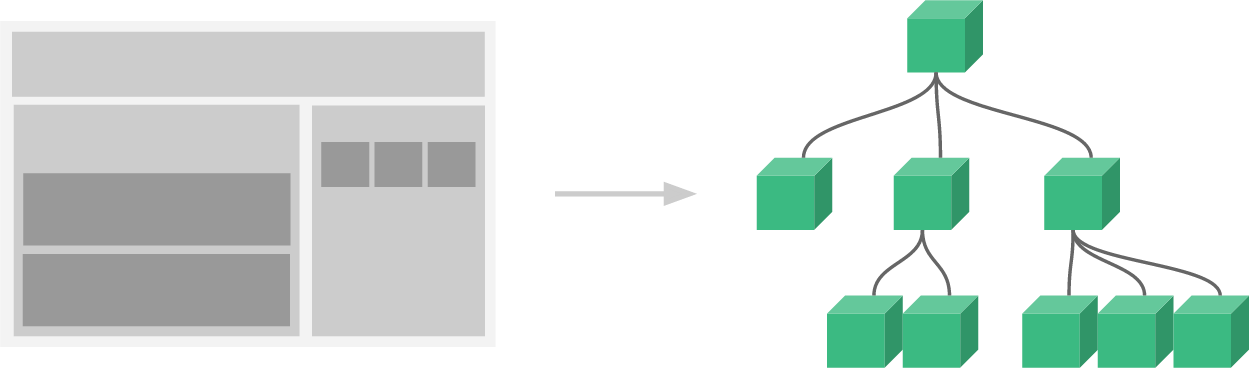
\includegraphics[scale=0.3]{components.png}
\caption{Vue.js组件系统}
\end{figure}

在一个大型应用中,为了使得开发过程可控,有必要将应用整体分割成一个个的组件。

\begin{lstlisting}[language=HTML]
<div id="app">
  <app-nav></app-nav>
  <app-view>
    <app-sidebar></app-sidebar>
    <app-content></app-content>
  </app-view>
</div>
\end{lstlisting}


Vue.js 组件非常类似于自定义元素——它是 Web 组件规范的一部分,而且实际上 Vue.js 的组件语法也参考了该规范。例如, Vue 组件实现了 Slot API 与 is 特性。

Vue.js组件和Web组件规范的关键的不同如下:

\begin{compactenum}
\item Web 组件规范仍然远未完成,并且没有浏览器实现。相比之下,Vue.js 组件不需要任何补丁,并且在所有支持的浏览器(IE9 及更高版本)之下表现一致。必要时,Vue.js 组件也可以放在原生自定义元素之内。
\item Vue.js 组件提供了原生自定义元素所不具备的一些重要功能,比如组件间的数据流,自定义事件系统,以及动态的、带特效的组件替换。
\end{compactenum}

在 Vue 里,一个组件实质上是一个拥有预定义选项的一个 Vue 实例:


\begin{lstlisting}[language=JavaScript]
// Define a new component called todo-item
Vue.component('todo-item', {
  template: '<li>This is a todo</li>'
})
\end{lstlisting}

在定义了一个组件之后就可以在另一个组件模板中写入它:

\begin{lstlisting}[language=HTML]
<ol>
  <!-- Create an instance of the todo-item component -->
  <todo-item></todo-item>
</ol>
\end{lstlisting}

最初,组件会为每个 todo 渲染同样的文本,实际上应该将数据从父作用域传到子组件,接下来可以修改组件的定义来让它能够接受一个 prop 字段:


\begin{lstlisting}[language=JavaScript]
Vue.component('todo-item',{
    // The todo-item component now accepts a
    // "prop", which is like a custom attribute.
    // This prop is called todo.
    props: ['todo'],
    template: '<li>{{ todo.text }}</li>
})
\end{lstlisting}

现在,可以使用 v-bind 指令将 todo 传到每一个重复的组件中:



\begin{lstlisting}[language=HTML]
<div id="app-7">
  <ol>
    <!-- Now we provide each todo-item with the todo object    -->
    <!-- it's representing, so that its content can be dynamic -->
    <todo-item v-for="item in groceryList" v-bind:todo="item"></todo-item>
  </ol>
</div>

Vue.component('todo-item', {
  props: ['todo'],
  template: '<li>{{ todo.text }}</li>'
})
var app7 = new Vue({
  el: '#app-7',
  data: {
    groceryList: [
      { text: 'Vegetables' },
      { text: 'Cheese' },
      { text: 'Whatever else humans are supposed to eat' }
    ]
  }
})
\end{lstlisting}


上述示例将应用分割成了两个更小的单元,子元素通过 props 接口实现了与父亲元素很好的解耦,现在可以在不影响到父应用的基础上,进一步为todo 组件改进更多复杂的模板和逻辑。


\section{Reactivity System}

组件系统(Component System)和响应式系统(Reactivity System)是Vue 最显著的两个特性。

在Vue.js响应式系统中,模型层(model)只是普通 JavaScript 对象,修改它则更新视图(view),从而可以让状态管理变得非常简单且直观。



\chapter{Vue Prop}


在 Vue.js 中,父子组件的关系可以总结为 props down, events up,父组件通过 props 向下传递数据给子组件,子组件通过 events 给父组件发送消息。

\begin{figure}[htbp]
\centering
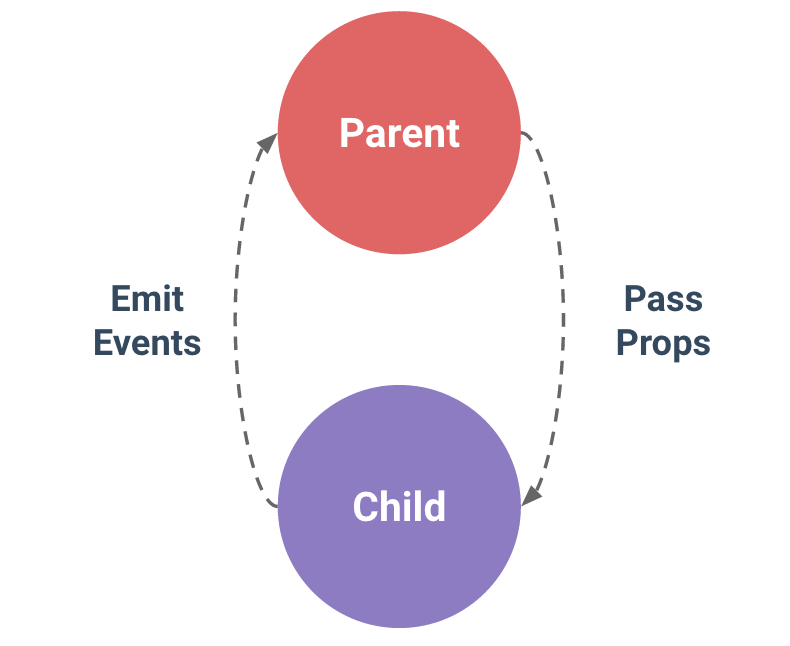
\includegraphics[scale=0.4]{props-events.png}
\caption{Vue.js的父子组件关系}
\end{figure}



\section{Prop}



组件实例的作用域是孤立的,这意味着不能并且不应该在子组件的模板内直接引用父组件的数据,Vue推荐使用 props 把数据传给子组件。


\begin{lstlisting}[language=JavaScript]
<div id="app">
    <child message="hello!"></child>
</div>
 
<script>
// 注册
Vue.component('child', {
  // 声明 props
  props: ['message'],
  // 同样也可以在 vm 实例中像 "this.message" 这样使用
  template: '<span>{{ message }}</span>'
})
// 创建根实例
new Vue({
  el: '#app'
})
</script>
\end{lstlisting}

最终渲染结果如下:


\begin{lstlisting}[language=JavaScript]
<div id="app">
    <span>hello!</span>
</div>
\end{lstlisting}

prop的本质是父组件用来传递数据的一个自定义属性。

\begin{compactitem}
\item 父组件的数据需要通过 props 把数据传给子组件;
\item 子组件需要显式地用 props 选项声明 "prop":
\end{compactitem}


\begin{lstlisting}[language=JavaScript]
Vue.component('child',{
   // 声明props
   props: ['message'],
   // 就像 data 一样,prop 可以用在模板内
   // 同样也可以在 vm 实例中像 “this.message” 这样使用
   template: '<span>{{ message }}</span>'
})
\end{lstlisting}

向它传入一个普通字符串:

\begin{lstlisting}[language=JavaScript]
<child message="hello!"></child>
\end{lstlisting}

下面是一个使用Prop向子组件传递数据的示例:

\begin{lstlisting}[language=JavaScript]
<div id="prop-example-1" class="demo">
  <child message="hello!"></child>
</div>
<script>
new Vue({
  el: '#prop-example-1',
  components: {
    child: {
      props: ['message'],
      template: '<span>{{ message }}</span>'
    }
  }
})
</script>
\end{lstlisting}


\subsection{Dynamic Prop}



动态Prop(Dynamic Prop)类似于用 v-bind 绑定 HTML 特性到一个表达式,也可以用 v-bind 动态绑定 props 的值到父组件的数据中,这样每当父组件的数据变化时,该变化也会传导给子组件:

\begin{lstlisting}[language=JavaScript]
<div>
  <input v-model="parentMsg"><br>
  <child v-bind:my-message="parentMsg"></child>
</div>

<script>
// 注册
Vue.component('child', {
  // 声明 props
  props: ['message'],
  // 同样也可以在 vm 实例中像 "this.message" 这样使用
  template: '<span>{{ message }}</span>'
})
// 创建根实例
new Vue({
  el: '#app',
  data: {
    parentMsg: '父组件内容'
  }
})
</script>
\end{lstlisting}

使用 v-bind 的缩写语法通常更简单:

\begin{lstlisting}[language=JavaScript]
<child :my-message="parentMsg"></child>
\end{lstlisting}

下面是一个动态Prop的示例:

\begin{lstlisting}[language=JavaScript]
<div id="demo">
  <input v-model="parentMsg">
  <br>
  <child v-bind:my-message="parentMsg"></child>
</div>

<script>
new Vue({
  el: '#demo',
  data: {
     parentMsg: 'Message from parent'
  },
  components: {
     child: {
        props: ['myMessage'],
        template: '<span>{{ myMessage }}</span>'
     }
  } 
})
</script>
\end{lstlisting}


以下实例中将 v-bind 指令将 todo 传到每一个重复的组件中:

\begin{lstlisting}[language=JavaScript]
<div id="app">
    <ol>
    <todo-item v-for="item in sites" v-bind:todo="item"></todo-item>
      </ol>
</div>
 
<script>
Vue.component('todo-item', {
  props: ['todo'],
  template: '<li>{{ todo.text }}</li>'
})
new Vue({
  el: '#app',
  data: {
    sites: [
      { text: 'Runoob' },
      { text: 'Google' },
      { text: 'Taobao' }
    ]
  }
})
</script>
\end{lstlisting}

\subsection{Literal Prop}


初学者常犯的一个错误是使用字面量语法传递数值:

\begin{lstlisting}[language=JavaScript]
<!-- 传递了一个字符串"1" -->
<comp some-prop="1"></comp>
\end{lstlisting}


因为它是一个字面 prop ,它的值以字符串 "1" 而不是以实际的数字传下去。


如果想传递一个实际的 JavaScript 数字,需要使用 v-bind ,这样可以让它的值被当作 JavaScript 表达式计算:



\begin{lstlisting}[language=JavaScript]
<!-- 传递实际的数字 -->
<comp v-bind:some-prop="1"></comp>
\end{lstlisting}


\section{Prop Flow}




prop 默认是单向绑定的,当父组件的属性变化时,将传导给子组件,但是不会反过来。

prop单向绑定的特性是为了防止子组件无意修改了父组件的状态——否则会让应用的数据流难以理解。

JavaScript中的对象和数组是引用类型,指向同一个内存空间,如果 prop 是一个对象或数组,在子组件内部改变它会影响父组件的状态。

每次父组件更新时,子组件的所有 prop 都会更新为最新值,这意味着不应该在子组件内部改变 prop,否则Vue 会在控制台给出警告。



通常有两种改变 prop 的情况:

\begin{compactenum}
\item prop 作为初始值传入,子组件之后只是将它的初始值作为本地数据的初始值使用;
\item prop 作为需要被转变的原始值传入。
\end{compactenum}

更确切的说,这两种情况是:

\begin{compactenum}
\item 定义一个局部 data 属性,并将 prop 的初始值作为局部数据的初始值。

\begin{lstlisting}[language=JavaScript]
props: ['initialCounter'],
data: function () {
  return { counter: this.initialCounter }
}
\end{lstlisting}

\item 定义一个 computed 属性,此属性从 prop 的值计算得出。

\begin{lstlisting}[language=JavaScript]
props: ['size'],
computed: {
  normalizedSize: function () {
    return this.size.trim().toLowerCase()
  }
}
\end{lstlisting}


\end{compactenum}



\section{Prop Validation}

组件可以为 props 指定验证要求。如果未指定验证要求,Vue 会发出警告。


prop 是一个对象而不是字符串数组时,它包含验证要求:



\begin{lstlisting}[language=JavaScript]
Vue.component('example', {
  props: {
    // 基础类型检测 (null的意思是任何类型都可以)
    propA: Number,
    // 多种类型
    propB: [String, Number],
    // 必传且是字符串
    propC: {
      type: String,
      required: true
    },
    // 数字,有默认值
    propD: {
      type: Number,
      default: 100
    },
    // 数组/对象的默认值应当由一个工厂函数返回
    propE: {
      type: Object,
      default: function () {
        return { message: 'hello' }
      }
    },
    // 自定义验证函数
    propF: {
      validator: function (value) {
        return value > 10
      }
    }
  }
})
\end{lstlisting}

type 可以是如下的原生构造器:

\begin{compactitem}
\item String
\item Number
\item Boolean
\item Function
\item Object
\item Array
\end{compactitem}

type 也可以是一个自定义构造器,使用 instanceof 检测。

如果prop验证失败,在Vue.js的开发版本中会抛出一条警告。

\chapter{Vue Event}

\section{Custom Event}


父组件默认使用 props 传递数据给子组件,如果子组件要把数据传递回去,需要使用自定义事件。




\subsection{Bind Custom Event}

在Vue.js中,可以使用 v-on 绑定自定义事件。

每个 Vue 实例都实现了事件接口(Events interface),即:

\begin{compactitem}
\item 使用 \$on(eventName) 监听事件
\item 使用 \$emit(eventName) 触发事件
\end{compactitem}

Vue的事件系统分离自浏览器的EventTarget API。尽管它们的运行类似,但是\$on 和 \$emit 不是addEventListener 和 dispatchEvent 的别名。

另外,父组件可以在使用子组件的地方直接用 v-on 来监听子组件触发的事件。




下面的示例中的子组件已经和它外部完全解耦了,它所做的只是触发一个父组件关心的内部事件。





\begin{lstlisting}[language=JavaScript]
<div id="counter-event-example">
  <p>{{ total }}</p>
  <button-counter v-on:increment="incrementTotal"></button-counter>
  <button-counter v-on:increment="incrementTotal"></button-counter>
</div>

<script>
Vue.component('button-counter', {
  template: '<button v-on:click="increment">{{ counter }}</button>',
  data: function () {
    return {
      counter: 0
    }
  },
  methods: {
    increment: function () {
      this.counter += 1
      this.$emit('increment')
    }
  },
})
new Vue({
  el: '#counter-event-example',
  data: {
    total: 0
  },
  methods: {
    incrementTotal: function () {
      this.total += 1
    }
  }
})
</script>
\end{lstlisting}



自定义事件也可以用来创建自定义的表单输入组件,必须使用 v-model 来进行数据双向绑定。


\begin{lstlisting}[language=JavaScript]
<input v-model="something">
\end{lstlisting}

v-model本身仅仅是一个语法糖:

\begin{lstlisting}[language=JavaScript]
<input v-bind:value="something" v-on:input="something = $event.target.value">
\end{lstlisting}

在组件中使用v-model时,相当于下面的简写:

\begin{lstlisting}[language=JavaScript]
<custom-input v-bind:value="something" v-on:input="something = arguments[0]"></custom-input>
\end{lstlisting}

要让组件的 v-model 生效,它必须:

\begin{compactitem}
\item 接受一个 value 属性
\item 在有新的 value 时触发 input 事件
\end{compactitem}

下面是一个非常简单的货币输入:

\begin{lstlisting}[language=JavaScript]
<div id="currency-input-example">
  <currency-input v-model="price"></currency-input>
</div>


Vue.component('currency-input', {
  template: '\
    <span>\
      $\
      <input\
        ref="input"\
        v-bind:value="value"\
        v-on:input="updateValue($event.target.value)"\
      >\
    </span>\
  ',
  props: ['value'],
  methods: {
    updateValue: function (value) {
      var formattedValue = value
        .trim()
        .slice(0, value.indexOf('.') + 3)
      if (formattedValue !== value) {
        this.$refs.input.value = formattedValue
      }
      this.$emit('input', Number(formattedValue))
    }
  }
})
new Vue({ el: '#currency-input-example' })
\end{lstlisting}


如果用户需要输入多个小数点或句号,则需要继续完善上述的货币过滤器。


\begin{lstlisting}[language=JavaScript]
<div id="app">
  <currency-input label="Price" v-model="price"></currency-input>
  <currency-input label="Shipping" v-model="shipping"></currency-input>
  <currency-input label="Handling" v-model="handling"></currency-input>
  <currency-input label="Discount" v-model="discount"></currency-input>
  <p>Total: ${{ total }}</p>
</div>

<script>
Vue.component('currency-input', {
  template: '\
    <div>\
      <label v-if="label">{{ label }}</label>\
      $\
      <input\
        ref="input"\
        v-bind:value="value"\
        v-on:input="updateValue($event.target.value)"\
        v-on:focus="selectAll"\
        v-on:blur="formatValue"\
      >\
    </div>\
  ',
  props: {
    value: {
      type: Number,
      default: 0
    },
    label: {
      type: String,
      default: ''
    }
  },
  mounted: function () {
    this.formatValue()
  },
  methods: {
    updateValue: function (value) {
      var result = currencyValidator.parse(value, this.value)
      if (result.warning) {
        this.$refs.input.value = result.value
      }
      this.$emit('input', result.value)
    },
    formatValue: function () {
      this.$refs.input.value = currencyValidator.format(this.value)
    },
    selectAll: function (event) {
      // Workaround for Safari bug
      // http://stackoverflow.com/questions/1269722/selecting-text-on-focus-using-jquery-not-working-in-safari-and-chrome
      setTimeout(function () {
      	event.target.select()
      }, 0)
    }
  }
})

new Vue({
  el: '#app',
  data: {
    price: 0,
    shipping: 0,
    handling: 0,
    discount: 0
  },
  computed: {
    total: function () {
      return ((
        this.price * 100 + 
        this.shipping * 100 + 
        this.handling * 100 - 
        this.discount * 100
      ) / 100).toFixed(2)
    }
  }
})
</script>
\end{lstlisting}


这个接口不仅仅可以用来连接组件内部的表单输入,也很容易集成自定义的输入类型。


\begin{lstlisting}[language=JavaScript]
<voice-recognizer v-model="question"></voice-recognizer>
<webcam-gesture-reader v-model="gesture"></webcam-gesture-reader>
<webcam-retinal-scanner v-model="retinalImage"></webcam-retinal-scanner>
\end{lstlisting}



\subsection{Bind Native Event}

如果需要在某个组件的根元素上监听一个原生事件,可以使用 .native 来修饰 v-on。


\begin{lstlisting}[language=JavaScript]
<my-component v-on:click.native="doTheThing"></my-component>
\end{lstlisting}



\section{Central Eventbus}

非父子关系的组件也需要通信时,简单的场景下可以使用一个空的 Vue 实例作为中央事件总线:



\begin{lstlisting}[language=JavaScript]
var bus = new Vue()
\end{lstlisting}

\begin{compactitem}
\item 触发组件 A 中的事件

\begin{lstlisting}[language=JavaScript]
// 触发组件 A 中的事件
bus.$emit('id-selected', 1)
\end{lstlisting}

\item 在组件 B 创建的钩子中监听事件

\begin{lstlisting}[language=JavaScript]
// 在组件 B 创建的钩子中监听事件
bus.$on('id-selected', function (id) {
  // ...
})
\end{lstlisting}
\end{compactitem}

在更复杂的情况下,应该考虑使用专门的 状态管理模式。


\chapter{Vue Slot}

组件经常需要组合进行使用,例如:

\begin{lstlisting}[language=JavaScript]
<app>
   <app-header></app-header>
   <app-footer></app-footer>
</app>
\end{lstlisting}

\begin{compactitem}
\item <app> 组件不知道它的挂载点会有什么内容。挂载点的内容是由<app>的父组件决定的。
\item <app> 组件很可能有它自己的模版。
\end{compactitem}

为了让组件可以组合,需要一种方式来混合父组件的内容与子组件自己的模板,这个过程被称为 内容分发(或 “transclusion”)。

在组合组件时,内容分发 API 是非常有用的机制,因此Vue.js参照 Web 组件规范草案实现了一个内容分发 API,可以使用特殊的 <slot> 元素作为原始内容的插槽。


\section{Compilation Scope}

首先,明确内容的编译作用域,假定模板为:


\begin{lstlisting}[language=JavaScript]
<child-component>
{{ message }}
</child-component>
\end{lstlisting}

这里的message 应该绑定到父组件的数据,组件作用域简单地说是:

\begin{compactitem}
\item 父组件模板的内容在父组件作用域内编译;
\item 子组件模板的内容在子组件作用域内编译。
\end{compactitem}

一个常见错误是试图在父组件模板内将一个指令绑定到子组件的属性/方法:


\begin{lstlisting}[language=JavaScript]
<!-- 无效 -->
<child-component v-show="someChildProperty"></child-component>
\end{lstlisting}

假定 someChildProperty 是子组件的属性,上例不会如预期那样工作,而且父组件模板不应该知道子组件的状态。

如果要绑定子组件内的指令到一个组件的根节点,应当在它的模板内这么做:

\begin{lstlisting}[language=JavaScript]
Vue.component('child-component',{
   //有效,在正确的作用域内
   template: '<div v-show="someChildProperty">Child</div>',
   data: function() {
      return someChildProperty: true
   }
})
\end{lstlisting}

类似地,分发内容是在父组件作用域内编译。


\section{Single Slot}


除非子组件模板包含至少一个 <slot> 插口,否则父组件的内容将会被丢弃。当子组件模板只有一个没有属性的 slot 时,父组件整个内容片段将插入到 slot 所在的 DOM 位置,并替换掉 slot 标签本身。

最初在 <slot> 标签中的任何内容都被视为备用内容。备用内容在子组件的作用域内编译,并且只有在宿主元素为空,且没有要插入的内容时才显示备用内容。

假定 my-component 组件有下面模板:

\begin{lstlisting}[language=JavaScript]
<div>
  <h2>我是子组件的标题</h2>
  <slot>
    只有在没有要分发的内容时才会显示。
  </slot>
</div>
\end{lstlisting}


父组件模版:


\begin{lstlisting}[language=JavaScript]
<div>
  <h1>我是父组件的标题</h1>
  <my-component>
    <p>这是一些初始内容</p>
    <p>这是更多的初始内容</p>
  </my-component>
</div>
\end{lstlisting}


渲染结果如下:


\begin{lstlisting}[language=JavaScript]
<div>
  <h1>我是父组件的标题</h1>
  <div>
    <h2>我是子组件的标题</h2>
    <p>这是一些初始内容</p>
    <p>这是更多的初始内容</p>
  </div>
</div>
\end{lstlisting}


\section{Named Slot}

<slot> 元素可以用一个特殊的属性 name 来配置如何分发内容。多个 slot 可以有不同的名字。具名 slot 将匹配内容片段中有对应 slot 特性的元素。

仍然可以有一个匿名 slot ,它是默认 slot ,作为找不到匹配的内容片段的备用插槽。如果没有默认的 slot ,这些找不到匹配的内容片段将被抛弃。

例如,假定有一个 app-layout 组件,它的模板为:

\begin{lstlisting}[language=JavaScript]
<div class="container">
  <header>
    <slot name="header"></slot>
  </header>
  <main>
    <slot></slot>
  </main>
  <footer>
    <slot name="footer"></slot>
  </footer>
</div>
\end{lstlisting}


父组件模版:


\begin{lstlisting}[language=JavaScript]
<app-layout>
  <h1 slot="header">这里可能是一个页面标题</h1>
  <p>主要内容的一个段落。</p>
  <p>另一个主要段落。</p>
  <p slot="footer">这里有一些联系信息</p>
</app-layout>
\end{lstlisting}


渲染结果为:


\begin{lstlisting}[language=JavaScript]
<div class="container">
  <header>
    <h1>这里可能是一个页面标题</h1>
  </header>
  <main>
    <p>主要内容的一个段落。</p>
    <p>另一个主要段落。</p>
  </main>
  <footer>
    <p>这里有一些联系信息</p>
  </footer>
</div>
\end{lstlisting}


\section{Scoped Slot}

作用域插槽是一种特殊类型的插槽,用作使用一个(能够传递数据到)可重用模板替换已渲染元素。

在子组件中,只需将数据传递到插槽,就像将 prop 传递给组件一样:

\begin{lstlisting}[language=JavaScript]
<div class="child">
  <slot text="hello from child"></slot>
</div>
\end{lstlisting}

在父级中,具有特殊属性 scope 的 <template> 元素,表示它是作用域插槽的模板。scope 的值对应一个临时变量名,此变量接收从子组件中传递的 prop 对象:



\begin{lstlisting}[language=JavaScript]
<div class="parent">
  <child>
    <template scope="props">
      <span>hello from parent</span>
      <span>{{ props.text }}</span>
    </template>
  </child>
</div>
\end{lstlisting}


渲染以上组件得到的输出如下:

\begin{lstlisting}[language=JavaScript]
<div class="parent">
  <div class="child">
    <span>hello from parent</span>
    <span>hello from child</span>
  </div>
</div>
\end{lstlisting}


作用域插槽更具代表性的用例是列表组件,允许组件自定义应该如何渲染列表每一项:

\begin{lstlisting}[language=JavaScript]
<my-awesome-list :items="items">
  <!-- 作用域插槽也可以在这里命名 -->
  <template slot="item" scope="props">
    <li class="my-fancy-item">{{ props.text }}</li>
  </template>
</my-awesome-list>
\end{lstlisting}

列表组件的模板:


\begin{lstlisting}[language=JavaScript]
<ul>
  <slot name="item"
    v-for="item in items"
    :text="item.text">
    <!-- fallback content here -->
  </slot>
</ul>
\end{lstlisting}




\begin{lstlisting}[language=JavaScript]

\end{lstlisting}





\begin{lstlisting}[language=JavaScript]

\end{lstlisting}





\begin{lstlisting}[language=JavaScript]

\end{lstlisting}






\begin{lstlisting}[language=JavaScript]

\end{lstlisting}





\begin{lstlisting}[language=JavaScript]

\end{lstlisting}





\begin{lstlisting}[language=JavaScript]

\end{lstlisting}





\begin{lstlisting}[language=JavaScript]

\end{lstlisting}





\begin{lstlisting}[language=JavaScript]

\end{lstlisting}





\chapter{Vue Rendering}



\section{Declarative Rendering}



Vue.js 的核心是一个允许采用简洁的模板语法来声明式的将数据渲染进 DOM 的系统:


\begin{lstlisting}[language=HTML]
<div>
  <p>{{ message }}</p>
</div>
\end{lstlisting}



\begin{lstlisting}[language=JavaScript]
var app = new Vue({
   el: '#app',
   data: {
      message: 'Hello, Vue.js!'
   }
})
\end{lstlisting}


最终渲染结果如下:

\begin{lstlisting}[language=HTML]
Hello, Vue.js!
\end{lstlisting}


虽然Vue.js渲染过程和渲染一个字符串模板非常类似,但是实际上Vue.js在背后做了大量工作。

Vue.js把数据和 DOM绑定在一起,所有的元素都是响应式的。例如,在浏览器的控制台中修改\texttt{app.message}将会看到相应地同步更新。

\subsection{v-bind}


除了绑定插入的文本内容,还可以采用这样的方式绑定 DOM 元素属性:


\begin{lstlisting}[language=HTML]
<div id="app-2">
  <span v-bind:title="message">
  Hover your mouse over me for a few seconds to see my dynamically bound title!
  </span>
</div>

<script>
var app2=new Vue({
   el: '#app-2',
   data: {
       message: 'You loaded this page on ` + new Date()
   }
})
<script>
\end{lstlisting}

v-bind 属性被称为指令。指令带有前缀 v-,以表示它们是 Vue.js 提供的特殊属性,它们会在渲染过的 DOM 上应用特殊的响应式行为。例如,这里的v-bind指令的简单含义是将这个元素节点的 title 属性和 Vue 实例的 message 属性绑定到一起。

在浏览器的控制台输入\texttt{app2.message = 'some new message'},就会再一次看到这个绑定了title属性的HTML已经进行了更新。



\section{Conditional Rendering}

\subsection{v-if}

在字符串模板(例如Handlebars)中,需要这样写一个条件块:


\begin{lstlisting}[language=JavaScript]
<!-- Handlebars 模板 -->
{{ #if ok}}
  <h1>Yes</h1>
{{/if}}
\end{lstlisting}

Vue.js的v-if 指令可以实现同样的功能:

\begin{lstlisting}[language=JavaScript]
<h1 v-if="ok">Yes</h1>
\end{lstlisting}

也可以用 v-else 添加一个 “else” 块:

\begin{lstlisting}[language=JavaScript]
<h1 v-if="ok">Yes</h1>
<h1 v-else>No</h1>
\end{lstlisting}

v-if 本身是一个指令,需要将它添加到一个元素上,如果想切换多个元素,可以把一个 <template> 元素当做包装元素,并在上面使用 v-if,最终的渲染结果不会包含它。


\begin{lstlisting}[language=JavaScript]
<template v-if="ok">
  <h1>Title</h1>
  <p>Paragraph 1</p>
  <p>Paragraph 2</p>
</template>
\end{lstlisting}



\begin{lstlisting}[language=JavaScript]

\end{lstlisting}



\begin{lstlisting}[language=JavaScript]

\end{lstlisting}


\subsection{v-else}

可以用 v-else 指令给 v-if 添加一个 “else” 块:


\begin{lstlisting}[language=JavaScript]
<div v-if="Math.random() > 0.5">
  Sorry
</div>
<div v-else>
  Not sorry
</div>
\end{lstlisting}

v-else 元素必须紧跟在 v-if 元素或者 v-else-if的后面——否则它不能被识别。

\begin{lstlisting}[language=JavaScript]

\end{lstlisting}



\begin{lstlisting}[language=JavaScript]

\end{lstlisting}


\subsection{v-else-if}

v-else-if,顾名思义,用作 v-if 的 else-if 块,可以链式的多次使用:

\begin{lstlisting}[language=JavaScript]
<div v-if="type === 'A'">
  A
</div>
<div v-else-if="type === 'B'">
  B
</div>
<div v-else-if="type === 'C'">
  C
</div>
<div v-else>
  Not A/B/C
</div>
\end{lstlisting}

与 v-else 相似,,v-else-if 必须跟在 v-if 或者 v-else-if之后。


Vue 尝试尽可能高效的渲染元素,通常会复用已有元素而不是从头开始渲染。这么做除了使 Vue 更快之外还可以得到一些好处。例如,为了允许用户在不同的登录方式之间切换:



\begin{lstlisting}[language=JavaScript]
<template v-if="loginType === 'username'">
  <label>Username</label>
  <input placeholder="Enter your username">
</template>
<template v-else>
  <label>Email</label>
  <input placeholder="Enter your email address">
</template>
\end{lstlisting}

在代码中切换 loginType 不会删除用户已经输入的内容,两个模版由于使用了相同的元素,<input> 会被复用,仅仅是替换了他们的 placeholder。

上述这种做法也不总是符合实际需求,所以 Vue 提供一种方式让浏览器可以自己决定是否要复用元素,开发者需要做的是添加一个属性 key ,key 必须带有唯一的值。

\begin{lstlisting}[language=JavaScript]
<template v-if="loginType === 'username'">
  <label>Username</label>
  <input placeholder="Enter your username" key="username-input">
</template>
<template v-else>
  <label>Email</label>
  <input placeholder="Enter your email address" key="email-input">
</template>
\end{lstlisting}

注意, <label> 元素仍然会被复用,因为没有被添加了 key 属性。


\subsection{v-show}

另一个根据条件展示元素的选项是 v-show 指令。


\begin{lstlisting}[language=JavaScript]
<h1 v-show="ok">Hello!</h1>
\end{lstlisting}

不同的是有 v-show 的元素会始终渲染并保持在 DOM 中。v-show 是简单的切换元素的 CSS 属性 display 。


注意,v-show 不支持 <template> 语法。

\begin{compactitem}
\item v-if 是真实的条件渲染,因为它会确保条件块在切换当中适当地销毁与重建条件块内的事件监听器和子组件。
\item v-if 也是惰性的:如果在初始渲染时条件为假,则什么也不做——在条件第一次变为真时才开始局部编译(编译会被缓存起来)。
\end{compactitem}


相比之下, v-show 简单得多——元素始终被编译并保留,只是简单地基于 CSS 切换。

一般来说, v-if 有更高的切换消耗而 v-show 有更高的初始渲染消耗,因此如果需要频繁切换使用 v-show 较好,如果在运行时条件不大可能改变则使用 v-if 较好。


\section{List Rendering}


当 Vue.js 用 v-for 正在更新已渲染过的元素列表时,它默认用 “就地复用” 策略。如果数据项的顺序被改变,Vue将不是移动 DOM 元素来匹配数据项的顺序, 而是简单复用此处每个元素,并且确保它在特定索引下显示已被渲染过的每个元素。这个类似 Vue 1.x 的 \texttt{track-by="\$index"} 。

这个默认的模式是有效的,但是只适用于不依赖子组件状态或临时 DOM 状态(例如表单输入值)的列表渲染输出。

为了给 Vue 一个提示,以便它能跟踪每个节点的身份,从而重用和重新排序现有元素,你需要为每项提供一个唯一 key 属性。理想的 key 值是每项都有唯一 id。这个特殊的属性相当于 Vue 1.x 的 track-by ,但它的工作方式类似于一个属性,所以需要用 v-bind 来绑定动态值(在这里使用简写):

建议尽可能使用 v-for 来提供 key ,除非迭代 DOM 内容足够简单,或者你是故意要依赖于默认行为来获得性能提升。


因为它是 Vue 识别节点的一个通用机制, key 并不特别与 v-for 关联,key 还具有其他用途。

\begin{lstlisting}[language=JavaScript]
<div v-for="item in items" :key="item.id">
  <!-- 内容 -->
</div>
\end{lstlisting}



\begin{lstlisting}[language=JavaScript]

\end{lstlisting}




\begin{lstlisting}[language=JavaScript]

\end{lstlisting}



\begin{lstlisting}[language=JavaScript]

\end{lstlisting}



\begin{lstlisting}[language=JavaScript]

\end{lstlisting}




\subsection{Array v-for}

v-for 指令根据一组数组的选项列表进行渲染。 v-for 指令需要以 \texttt{item in items}形式的特殊语法,其中 items 是源数据数组并且 item 是数组元素迭代的别名。

\begin{lstlisting}[language=JavaScript]
<ul id="example-1">
  <li v-for="item in items">
    {{ item.message }}
  </li>
</ul>

<script>
var example1 = new Vue({
  el: '#example-1',
  data: {
    items: [
      {message: 'Foo' },
      {message: 'Bar' }
    ]
  }
})
</script>
\end{lstlisting}

渲染结果如下:


\begin{lstlisting}[language=JavaScript]
<ul id="example-1" class="demo">
  <li>Foo</li>
  <li>Bar</li>
</ul>
\end{lstlisting}


在 v-for 块中,我们拥有对父作用域属性的完全访问权限,而且v-for 还支持一个可选的第二个参数为当前项的索引。





\begin{lstlisting}[language=JavaScript]
<ul id="example-2">
  <li v-for="(item, index) in items">
    {{ parentMessage }} - {{ index }} - {{ item.message }}
  </li>
</ul>

<script>
var example2 = new Vue({
  el: '#example-2',
  data: {
    parentMessage: 'Parent',
    items: [
      { message: 'Foo' },
      { message: 'Bar' }
    ]
  }
})
</script>
\end{lstlisting}

渲染结果如下:

\begin{lstlisting}[language=JavaScript]
<ul id="example-2" class="demo">
  <li>Parent - 0 - Foo</li>
  <li>Parent - 1 - Bar</li>
</ul>
\end{lstlisting}

也可以用 of 替代 in 作为分隔符,因为它是最接近 JavaScript 迭代器的语法:

\begin{lstlisting}[language=JavaScript]
<div v-for="item of items"></div>
\end{lstlisting}


\subsection{Template v-for}


和v-if 模板一样,也可以用带有 v-for 的 <template> 标签来渲染多个元素块。例如:

\begin{lstlisting}[language=JavaScript]
<ul>
  <template v-for="item in items">
    <li>{{ item.msg }}</li>
    <li class="divider"></li>
  </template>
</ul>
\end{lstlisting}

\subsection{Object v-for}

也可以用 v-for 通过一个对象的属性来迭代。


\begin{lstlisting}[language=JavaScript]
<ul id="repeat-object" class="demo">
  <li v-for="value in object">
    {{ value }}
  </li>
</ul>

<script>
new Vue({
  el: '#repeat-object',
  data: {
    object: {
      FirstName: 'John',
      LastName: 'Doe',
      Age: 30
    }
  }
})
</script>
\end{lstlisting}

渲染结果如下:

\begin{lstlisting}[language=JavaScript]
<ul id="repeat-object" class="demo">
   <li>John</li>
   <li>Doe</li>
   <li>30</li>
</ul>
\end{lstlisting}

也可以提供第二个的参数为键名:


\begin{lstlisting}[language=JavaScript]
<div v-for="(value, key) in object">
  {{ key }} : {{ value }}
</div>
\end{lstlisting}

第三个参数为索引:

\begin{lstlisting}[language=JavaScript]
<div v-for="(value, key, index) in object">
  {{ index }}. {{ key }} : {{ value }}
</div>
\end{lstlisting}

在遍历对象时,是按 Object.keys() 的结果遍历,但是不能保证它的结果在不同的 JavaScript 引擎下是一致的。

\subsection{Integer v-for}

v-for 也可以取整数。在这种情况下,它将重复多次模板。


\begin{lstlisting}[language=JavaScript]
<div>
  <span v-for="n in 10">{{ n }}</span>
</div>
\end{lstlisting}



渲染结果如下:


\begin{lstlisting}[language=JavaScript]
<div id="range" class="demo">
  <span>1 </span>
  <span>2 </span>
  <span>3 </span>
  <span>4 </span>
  <span>5 </span>
  <span>6 </span>
  <span>7 </span>
  <span>8 </span>
  <span>9 </span>
  <span>10 </span>
</div>
\end{lstlisting}

\subsection{Component v-for}

在自定义组件里,可以像任何普通元素一样用 v-for 。

\begin{lstlisting}[language=JavaScript]
<my-component v-for="item in items"></my-component>
\end{lstlisting}

但是,默认不能自动传递数据到组件里,因为组件有自己独立的作用域。

为了传递迭代数据到组件里,这里需要用 props :

\begin{lstlisting}[language=JavaScript]
<my-component
  v-for="(item, index) in items"
  v-bind:item="item"
  v-bind:index="index">
</my-component>
\end{lstlisting}


不自动注入 item 到组件里的原因是,因为这使得组件会紧密耦合到 v-for 如何运作。

在一些情况下,明确数据的来源可以使组件可重用。

下面是一个简单的 todo list 完整的例子:


\begin{lstlisting}[language=JavaScript]
<div id="todo-list-example">
  <input
    v-model="newTodoText"
    v-on:keyup.enter="addNewTodo"
    placeholder="Add a todo"
  >
  <ul>
    <li
      is="todo-item"
      v-for="(todo, index) in todos"
      v-bind:title="todo"
      v-on:remove="todos.splice(index, 1)"
    ></li>
  </ul>
</div>

<script>
Vue.component('todo-item', {
  template: '\
    <li>\
      {{ title }}\
      <button v-on:click="$emit(\'remove\')">X</button>\
    </li>\
  ',
  props: ['title']
})
new Vue({
  el: '#todo-list-example',
  data: {
    newTodoText: '',
    todos: [
      'Do the dishes',
      'Take out the trash',
      'Mow the lawn'
    ]
  },
  methods: {
    addNewTodo: function () {
      this.todos.push(this.newTodoText)
      this.newTodoText = ''
    }
  }
})
</script>
\end{lstlisting}

\chapter{Vue Array}

Vue 包含一组观察数组的变异方法,所以它们也将会触发视图更新。这些方法如下:

\begin{compactitem}
\item push()
\item pop()
\item shift()
\item unshift()
\item splice()
\item sort()
\item reverse()
\end{compactitem}

例如,可以打开控制台,然后用前面例子的 items 数组调用变异方法:


\begin{lstlisting}[language=JavaScript]
example1.items.push({ message: 'Baz' })
\end{lstlisting}


\section{push()}


\section{pop()}

\section{shift()}


\section{unshift()}

\section{splice()}

\section{sort()}

\section{reverse()}

\section{filter()}

变异方法(mutation method),顾名思义,会改变被这些方法调用的原始数组。相比之下,也有非变异(non-mutating method)方法,例如filter(), concat(), slice() 。这些不会改变原始数组,但总是返回一个新数组。

当使用非变异方法时,可以用新数组替换旧数组:


\begin{lstlisting}[language=JavaScript]
example1.items = example1.items.filter(function (item) {
  return item.message.match(/Foo/)
})
\end{lstlisting}

可能认为这将导致 Vue 丢弃现有 DOM 并重新渲染整个列表。幸运的是,事实并非如此。 Vue 实现了一些智能启发式方法来最大化 DOM 元素重用,所以用一个含有相同元素的数组去替换原来的数组是非常高效的操作。


由于 JavaScript 的限制, Vue 不能检测以下变动的数组:

\begin{compactenum}
\item 当利用索引直接设置一个项时,例如\texttt{vm.items[indexOfItem] = newValue}
\item 当修改数组的长度时,例如\texttt{vm.items.length = newLength}
\end{compactenum}


为了避免第一种情况,以下两种方式将达到像 \texttt{vm.items[indexOfItem] = newValue}的效果, 同时也将触发状态更新:

\begin{compactitem}
\item 方式1

\begin{lstlisting}[language=JavaScript]
// Vue.set
Vue.set(example1.items, indexOfItem, newValue)
\end{lstlisting}

\item 方式2

\begin{lstlisting}[language=JavaScript]
// Array.prototype.splice`
example1.items.splice(indexOfItem, 1, newValue)
\end{lstlisting}

\end{compactitem}

要避免第二种情况,使用 splice:





\begin{lstlisting}[language=JavaScript]
example1.items.splice(newLength)
\end{lstlisting}

如果需要显示一个数组的过滤或排序副本,而不实际改变或重置原始数据。在这种情况下,可以创建返回过滤或排序数组的计算属性。

\begin{lstlisting}[language=JavaScript]
<li v-for="n in evenNumbers">{{ n }}</li>

<script>
data: {
  numbers: [ 1, 2, 3, 4, 5 ]
},
computed: {
  evenNumbers: function () {
    return this.numbers.filter(function (number) {
      return number % 2 === 0
    })
  }
}
</script>
\end{lstlisting}

或者,也可以在计算属性不适用的情况下 (例如在嵌套 v-for 循环中) 使用 method 方法:

\begin{lstlisting}[language=JavaScript]
<li v-for="n in even(numbers)">{{ n }}</li>

<script>
data: {
  numbers: [ 1, 2, 3, 4, 5 ]
},
methods: {
  even: function (numbers) {
    return numbers.filter(function (number) {
      return number % 2 === 0
    })
  }
}
</script>
\end{lstlisting}



\section{concat()}

\section{slice()}



\chapter{Vue Form}




\section{v-model}


v-model 指令可以在表单控件元素上创建双向数据绑定。

v-model会根据控件类型自动选取正确的方法来更新元素,v-model 本质上不过是语法糖,它负责监听用户的输入事件以更新数据,并特别处理一些极端的例子。


v-model 并不关心表单控件初始化所生成的值。因为它会选择 Vue 实例数据来作为具体的值。

For languages that require an IME (Chinese, Japanese, Korean etc.), you’ll notice that v-model doesn’t get updated during IME composition. If you want to cater for these updates as well, use input event instead.

如果HTML 内建的 input 类型不能满足需求,Vue 的组件系统允许创建一个具有自定义行为可复用的 input 类型,这些 input 类型可以和 v-model 一起使用。

\subsection{Input}


\begin{lstlisting}[language=JavaScript]
<div id="example-1">
  <input v-model="message" placeholder="edit me">
  <p>Message is: {{ message }}</p>
</div>

<script>
new Vue({
  el: "example-1",
  data: {
     message: ''
  }
})
</script>
\end{lstlisting}

\subsection{Textarea}


\begin{lstlisting}[language=JavaScript]
<div id="example-textarea" class="demo">
  <span>Multiline message is:</span> 
  <p style="white-space: pre;">{{ message }}</p> <br> 
  <textarea v-model="message" placeholder="add multiple lines"></textarea>
</div>
<script>
new Vue({
  el: '#example-textarea',
  data: {
    message: ''
  }
})
</script>
\end{lstlisting}

在文本区域插值( <textarea></textarea> ) 并不会生效,应用 v-model 来代替

\subsection{Checkbox}

单个勾选框,逻辑值:


\begin{lstlisting}[language=JavaScript]
<div id="example-2" class="demo">
<input type="checkbox" id="checkbox" v-model="checked"> 
<label for="checkbox">{{ checked }}</label>
</div>

<script>
new Vue({
  el: '#example-2',
  data: {
    checked: false
  }
})
</script>
\end{lstlisting}

多个勾选框,绑定到同一个数组:





\begin{lstlisting}[language=JavaScript]
<div id="example-3" class="demo">
  <input type="checkbox" id="jack" value="Jack" v-model="checkedNames"> 
  <label for="jack">Jack</label> 
  <input type="checkbox" id="john" value="John" v-model="checkedNames"> 
  <label for="john">John</label> 
  <input type="checkbox" id="mike" value="Mike" v-model="checkedNames"> 
  <label for="mike">Mike</label> <br> 
  <span>Checked names: {{ checkedNames }}</span>
</div>

<script>
new Vue({
  el: '#example-3',
  data: {
    checkedNames: []
  }
})
</script>
\end{lstlisting}

\subsection{Radio}


\begin{lstlisting}[language=JavaScript]
<div id="example-4" class="demo">
  <input type="radio" id="one" value="One" v-model="picked"> 
  <label for="one">One</label> <br> 
  <input type="radio" id="two" value="Two" v-model="picked"> 
  <label for="two">Two</label> <br> 
  <span>Picked: {{ picked }}</span>
</div>

<script>
new Vue({
  el: '#example-4',
  data: {
    picked: ''
  }
})
</script>
\end{lstlisting}



\subsection{Single Select}



\begin{lstlisting}[language=JavaScript]
<div id="example-5" class="demo">
<select v-model="selected">
  <option>A</option> 
  <option>B</option> 
  <option>C</option>
</select> 
<span>Selected: {{ selected }}</span>
</div>

<script>
new Vue({
  el: '#example-5',
  data: {
    selected: null
  }
})
</script>
\end{lstlisting}


\subsection{Multiple Select}


绑定到一个数组。



\begin{lstlisting}[language=JavaScript]
<select v-model="selected" multiple>
  <option>A</option>
  <option>B</option>
  <option>C</option>
</select>
<br>
<span>Selected: {{ selected }}</span>

<script>
new Vue({
  el: '#example-6',
  data: {
    selected: []
  }
})
</script>
\end{lstlisting}

动态选项,用 v-for 渲染:


\begin{lstlisting}[language=JavaScript]
<select v-model="selected">
  <option v-for="option in options" v-bind:value="option.value">
    {{ option.text }}
  </option>
</select>
<span>Selected: {{ selected }}</span>

<script>
new Vue({
  el: '#example-7',
  data: {
    selected: 'A',
    options: [
      { text: 'One', value: 'A' },
      { text: 'Two', value: 'B' },
      { text: 'Three', value: 'C' }
    ]
  }
})
</script>
\end{lstlisting}

对于单选按钮,勾选框及选择列表选项, v-model 绑定的 value 通常是静态字符串(对于勾选框是逻辑值):


\begin{lstlisting}[language=JavaScript]
<!-- 当选中时,`picked` 为字符串 "a" -->
<input type="radio" v-model="picked" value="a">
<!-- `toggle` 为 true 或 false -->
<input type="checkbox" v-model="toggle">
<!-- 当选中时,`selected` 为字符串 "abc" -->
<select v-model="selected">
  <option value="abc">ABC</option>
</select>
\end{lstlisting}

\section{v-bind}


在某些情况下,如果想绑定 value 到 Vue 实例的一个动态属性上,这时可以用 v-bind 实现,并且这个属性的值可以不是字符串。


\subsection{Checkbox}






\begin{lstlisting}[language=JavaScript]
<input
  type="checkbox"
  v-model="toggle"
  v-bind:true-value="a"
  v-bind:false-value="b"
>
\end{lstlisting}



\begin{lstlisting}[language=JavaScript]
// 当选中时
vm.toggle === vm.a
// 当没有选中时
vm.toggle === vm.b
\end{lstlisting}

\subsection{Radio}


\begin{lstlisting}[language=JavaScript]
<input type="radio" v-model="pick" v-bind:value="a">
\end{lstlisting}




\begin{lstlisting}[language=JavaScript]
// 当选中时
vm.pick === vm.a
\end{lstlisting}

\subsection{Select}


\begin{lstlisting}[language=JavaScript]
<select v-model="selected">
    <!-- 内联对象字面量 -->
  <option v-bind:value="{ number: 123 }">123</option>
</select>
\end{lstlisting}



\begin{lstlisting}[language=JavaScript]
// 当选中时
typeof vm.selected // -> 'object'
vm.selected.number // -> 123
\end{lstlisting}



\section{Modifier}


\subsection{.lazy}

在默认情况下, v-model 在 input 事件中同步输入框的值与数据 (除了 上述 IME 部分),但是可以添加一个修饰符 lazy ,从而转变为在 change 事件中同步:

\begin{lstlisting}[language=JavaScript]
<!-- 在 "change" 而不是 "input" 事件中更新 -->
<input v-model.lazy="msg" >
\end{lstlisting}





\begin{lstlisting}[language=JavaScript]

\end{lstlisting}


\subsection{.number}

如果想自动将用户的输入值转为 Number 类型(如果原值的转换结果为 NaN 则返回原值),可以添加一个修饰符 number 给 v-model 来处理输入值:

\begin{lstlisting}[language=JavaScript]
<input v-model.number="age" type="number">
\end{lstlisting}


这通常很有用,因为在 type="number" 时 HTML 中输入的值也总是会返回字符串类型。


\begin{lstlisting}[language=JavaScript]

\end{lstlisting}


\subsection{.trim}

如果要自动过滤用户输入的首尾空格,可以添加 trim 修饰符到 v-model 上过滤输入:

\begin{lstlisting}[language=JavaScript]
<input v-model.trim="msg">
\end{lstlisting}





\begin{lstlisting}[language=JavaScript]

\end{lstlisting}




\begin{lstlisting}[language=JavaScript]

\end{lstlisting}





\begin{lstlisting}[language=JavaScript]

\end{lstlisting}




\begin{lstlisting}[language=JavaScript]

\end{lstlisting}





\begin{lstlisting}[language=JavaScript]

\end{lstlisting}


\chapter{Vue Instance}

\section{Contructor}

每个 Vue.js 应用(即Vue VM)都是通过构造函数 Vue 创建一个 Vue 的根实例 启动的。

所有的 Vue.js 组件其实都是被扩展的 Vue 实例。


\begin{lstlisting}[language=JavaScript]
var vm = new Vue({
   // 选项
})
\end{lstlisting}


 Vue 的设计受到了MVVM模式的启发,因此在Vue中使用 vm 这个变量名表示 Vue 实例。
 
 

 
 \section{Option Object}


在实例化 Vue 时,需要传入一个选项对象,它可以包含数据、模板、挂载元素、方法、生命周期钩子等选项。

\subsection{el}


\subsection{data}


使用组件时,大多数可以传入到 Vue 构造器中的选项(options)可以在注册组件时使用,只有一个例外—— data。

data必须是一个函数,否则Vue 会在控制台发出警告,说明在组件中 data 必须是一个函数,因此最好理解这种规则的存在意义。



\begin{lstlisting}[language=JavaScript]
Vue.component('my-component', {
  template: '<span>{{ message }}</span>',
  data: {
    message: 'hello'
  }
})
\end{lstlisting}

在使用上述的Vue组件时,Vue会在控制台发出警告说明Vue组件中的data必须是一个函数。

\begin{lstlisting}[language=JavaScript]
<div id="example-2">
  <simple-counter></simple-counter>
  <simple-counter></simple-counter>
  <simple-counter></simple-counter>
</div>

<script>
var data = { counter: 0 }
Vue.component('simple-counter', {
  template: '<button v-on:click="counter += 1">{{ counter }}</button>',
  // data 是一个函数,因此 Vue 不会警告,
  // 但是我们为每一个组件返回了同一个对象引用
  data: function () {
    return data
  }
})
new Vue({
  el: '#example-2'
})
</script>
\end{lstlisting}

上述的这三个组件共享了同一个 data , 因此会导致增加一个 counter 会影响所有组件,可以通过为每个组件返回新的 data 对象来解决这个问题,这样每个 counter 都有它自己内部的状态了:

\begin{lstlisting}[language=JavaScript]
data: function () {
  return {
    counter: 0
  }
}
\end{lstlisting}




\begin{lstlisting}[language=JavaScript]

\end{lstlisting}




\begin{lstlisting}[language=JavaScript]

\end{lstlisting}





\begin{lstlisting}[language=JavaScript]

\end{lstlisting}




\subsection{template}


\subsection{methods}




\section{Extend Contructor}


可以扩展 Vue 构造器,从而用预定义选项创建可复用的组件构造器:


\begin{lstlisting}[language=JavaScript]
var MyComponent = Vue.extend({
   // 扩展选项
})

// 所有的 `MyComponent` 实例都将以预定义的扩展选项被创建
var myComponentInstance = new MyComponent()
\end{lstlisting}


尽管可以命令式地创建扩展实例,不过在多数情况下建议将组件构造器注册为一个自定义元素,然后声明式地用在模板中。

\section{Property}

\subsection{data}

每个 Vue 实例都会代理其 data 对象里所有的属性:

\begin{lstlisting}[language=JavaScript]
var data = { a: 1 }
var vm = new Vue({
  data: data
})
vm.a === data.a // -> true
// 设置属性也会影响到原始数据
vm.a = 2
data.a // -> 2
// ... 反之亦然
data.a = 3
vm.a // -> 3
\end{lstlisting}

注意,只有这些被代理的属性是响应的。如果在实例创建之后添加新的属性到实例上,它不会触发视图更新。

除了 data 属性, Vue 实例暴露了一些有用的实例属性与方法。这些属性与方法都有前缀 \$,以便与代理的 data 属性区分。例如:

\begin{lstlisting}[language=JavaScript]
var data = { a: 1 }
var vm = new Vue({
  el: '#example',
  data: data
})
vm.$data === data // -> true
vm.$el === document.getElementById('example') // -> true
// $watch 是一个实例方法
vm.$watch('a', function (newVal, oldVal) {
  // 这个回调将在 `vm.a`  改变后调用
})
\end{lstlisting}

注意,不要在实例属性或者回调函数中(如 \texttt{vm.\$watch('a', newVal => this.myMethod())})使用箭头函数。因为箭头函数绑定父上下文,所以 this 不会像预想的一样是 Vue 实例,而是 \texttt{this.myMethod} 未被定义。

\section{Method}


\section{Lifecycle}

\begin{figure}[htbp]
\centering
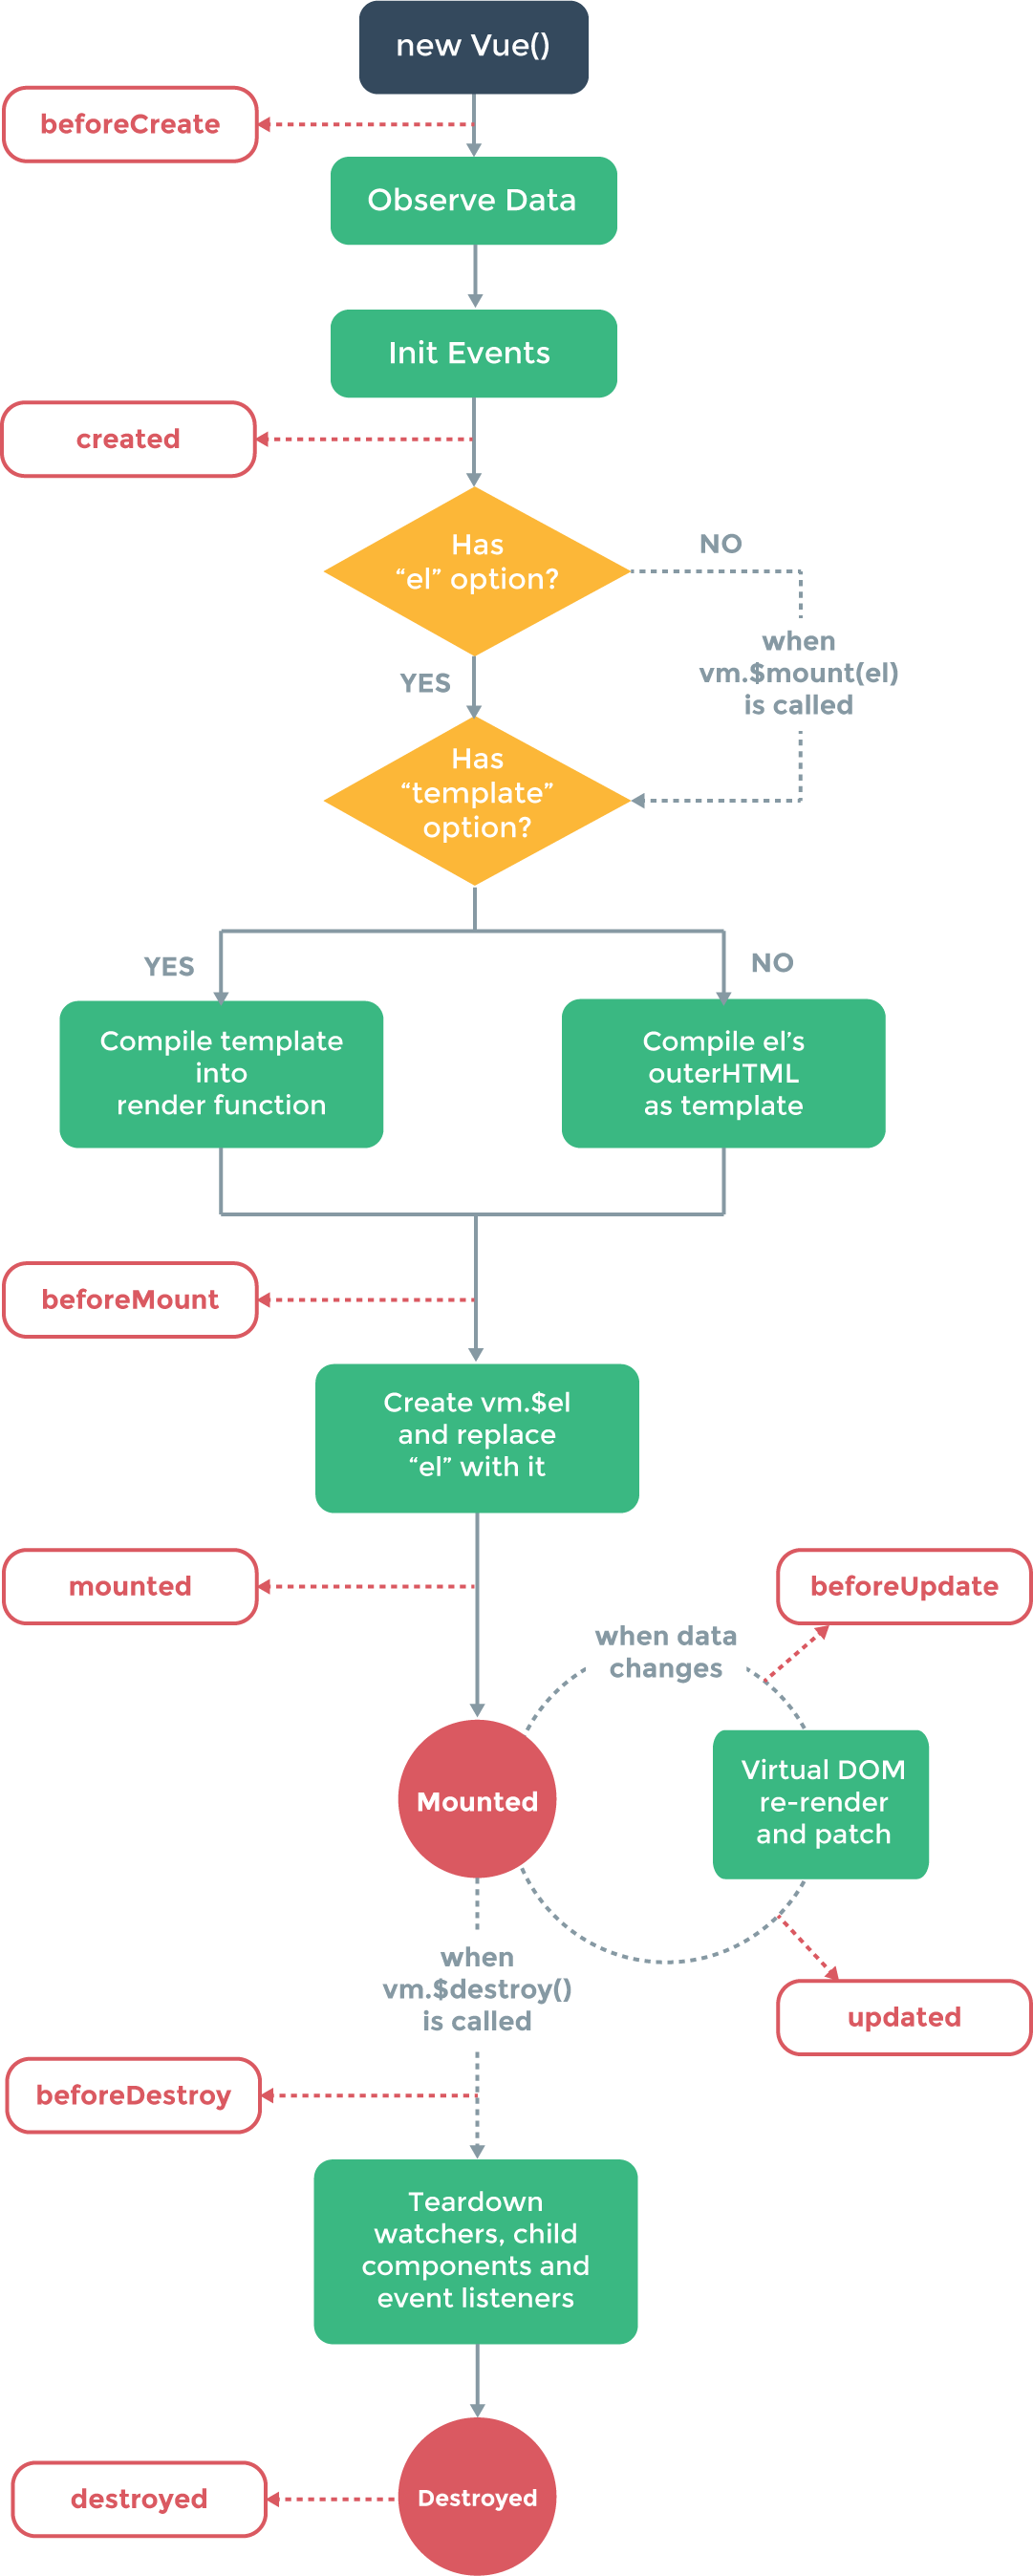
\includegraphics[scale=0.25]{lifecycle.png}
\caption{Vue实例的生命周期}
\end{figure}

每个 Vue 实例在被创建之前都要经过一系列的初始化过程。例如,实例需要配置数据观测(data observer)、编译模版、挂载实例到 DOM ,然后在数据变化时更新 DOM 。


\subsection{beforeCreate}


\subsection{created}


在Vue实例被创建的过程中,实例也会调用一些 生命周期钩子 ,这就给我们提供了执行自定义逻辑的机会。例如,created 这个钩子在实例被创建之后被调用:

\begin{lstlisting}[language=JavaScript]
var vm = new Vue({
  data: {
    a: 1
  },
  created: function () {
    // `this` 指向 vm 实例
    console.log('a is: ' + this.a)
  }
})
// -> "a is: 1"
\end{lstlisting}


\subsection{beforeUpdate}


\subsection{updated}




\subsection{beforeMount}



\subsection{mounted}


也有一些其它的钩子,在实例生命周期的不同阶段调用,如 mounted、 updated 、destroyed 。钩子的 this 指向调用它的 Vue 实例。

\subsection{beforeDestroy}


\subsection{destroyed}



Vue.js没有“控制器”的概念,组件的自定义逻辑可以分布在这些钩子中。

\chapter{Vue Template}


Vue.js 使用了基于 HTML 的模版语法,允许开发者声明式地将 DOM 绑定至底层 Vue 实例的数据。所有 Vue.js 的模板都是合法的 HTML ,所以能被遵循规范的浏览器和 HTML 解析器解析。


在底层的实现上, Vue 将模板编译成虚拟 DOM 渲染函数。结合响应系统,在应用状态改变时, Vue 能够智能地计算出重新渲染组件的最小代价并应用到 DOM 操作上。

如果熟悉虚拟 DOM,可以结合原生JavaScript代码,从而在不用模板,直接写渲染(render)函数,使用可选的 JSX 语法。



\begin{lstlisting}[language=JavaScript]

\end{lstlisting}





\begin{lstlisting}[language=JavaScript]

\end{lstlisting}




\begin{lstlisting}[language=JavaScript]

\end{lstlisting}

\section{Interpolation}


\subsection{Text}

数据绑定最常见的形式就是使用 “Mustache” 语法(双大括号)的文本插值:

\begin{lstlisting}[language=JavaScript]
<span>Message: {{ msg }}</span>
\end{lstlisting}

Mustache 标签将会被替代为对应数据对象上 msg 属性的值。无论何时,绑定的数据对象上 msg 属性发生了改变,插值处的内容都会更新。




通过使用 v-once 指令,你也能执行一次性地插值,当数据改变时,插值处的内容不会更新。但请留心这会影响到该节点上所有的数据绑定:

\begin{lstlisting}[language=JavaScript]
<span v-once>This will never change: {{ msg }}</span>
\end{lstlisting}




\subsection{HTML}

双大括号会将数据解释为纯文本,而非 HTML 。为了输出真正的 HTML ,你需要使用 v-html 指令:

\begin{lstlisting}[language=JavaScript]
<div v-html="rawHtml"></div>
\end{lstlisting}

被插入的内容都会被当做 HTML —— 数据绑定会被忽略。注意,你不能使用 v-html 来复合局部模板,因为 Vue 不是基于字符串的模板引擎。组件更适合担任 UI 重用与复合的基本单元。

站点上动态渲染的任意 HTML 可能会非常危险,因为它很容易导致 XSS 攻击。请只对可信内容使用 HTML 插值,绝不要对用户提供的内容插值。




\subsection{Attribute}

Mustache 不能在 HTML 属性中使用,应使用 v-bind 指令:

\begin{lstlisting}[language=JavaScript]
<div v-bind:id="dynamicId"></div>
\end{lstlisting}

这对布尔值的属性也有效 —— 如果条件被求值为 false 的话该属性会被移除:

\begin{lstlisting}[language=JavaScript]
<button v-bind:disabled="someDynamicCondition">Button</button>
\end{lstlisting}





\subsection{Expression}

在模板中除了绑定简单的属性键值之外,对于所有的数据绑定, Vue.js 都提供了完全的 JavaScript 表达式支持。

\begin{lstlisting}[language=JavaScript]
{{ number + 1 }}
{{ ok ? 'YES' : 'NO' }}
{{ message.split('').reverse().join('') }}
<div v-bind:id="'list-' + id"></div>
\end{lstlisting}


这些表达式会在所属 Vue 实例的数据作用域下作为 JavaScript 被解析。有个限制就是,每个绑定都只能包含单个表达式,所以下面的例子都不会生效。

\begin{lstlisting}[language=JavaScript]
<!-- 这是语句,不是表达式 -->
{{ var a = 1 }}
<!-- 流控制也不会生效,请使用三元表达式 -->
{{ if (ok) { return message } }}
\end{lstlisting}


模板表达式都被放在沙盒中,只能访问全局变量的一个白名单,如 Math 和 Date 。你不应该在模板表达式中试图访问用户定义的全局变量。




\section{Directive}

指令(Directives)是带有 v- 前缀的特殊属性。指令属性的值预期是单一 JavaScript 表达式(除了 v-for,之后再讨论)。指令的职责就是当其表达式的值改变时相应地将某些行为应用到 DOM 上。

\begin{lstlisting}[language=JavaScript]
<p v-if="seen">Now you see me</p>
\end{lstlisting}

这里, v-if 指令将根据表达式 seen 的值的真假来移除/插入 <p> 元素。


\begin{lstlisting}[language=JavaScript]

\end{lstlisting}




\subsection{Argument}

一些指令能接受一个“参数”,在指令后以冒号指明。例如, v-bind 指令被用来响应地更新 HTML 属性:

\begin{lstlisting}[language=JavaScript]
<a v-bind:href="url"></a>
\end{lstlisting}

在这里 href 是参数,告知 v-bind 指令将该元素的 href 属性与表达式 url 的值绑定。

另一个例子是 v-on 指令,它用于监听 DOM 事件:

\begin{lstlisting}[language=JavaScript]
<a v-on:click="doSomething">
\end{lstlisting}

在这里参数是监听的事件名。

\subsection{Modifier}

修饰符(Modifiers)是以半角句号 . 指明的特殊后缀,用于指出一个指定应该以特殊方式绑定。例如,.prevent 修饰符告诉 v-on 指令对于触发的事件调用 event.preventDefault():

\begin{lstlisting}[language=JavaScript]
<form v-on:submit.prevent="onSubmit"></form>
\end{lstlisting}


\section{Filter}

Vue.js allows you to define filters that can be used to apply common text formatting. Filters are usable in two places: mustache interpolations and v-bind expressions. Filters should be appended to the end of the JavaScript expression, denoted by the “pipe” symbol:

Vue.js 允许自定义过滤器,被用作一些常见的文本格式化。过滤器应该被添加在 mustache 插值的尾部,由“管道符”指示:


\begin{lstlisting}[language=JavaScript]
{{ message | capitalize }}
\end{lstlisting}




\begin{lstlisting}[language=JavaScript]
<!-- in mustaches -->
{{ message | capitalize }}
<!-- in v-bind -->
<div v-bind:id="rawId | formatId"></div>
\end{lstlisting}


Vue 2.x 中,过滤器只能在 mustache 绑定和 v-bind 表达式(从 2.1.0 开始支持)中使用,因为过滤器设计目的就是用于文本转换。为了在其他指令中实现更复杂的数据变换,你应该使用计算属性。

过滤器函数总接受表达式的值作为第一个参数。



\begin{lstlisting}[language=JavaScript]
new Vue({
  // ...
  filters: {
    capitalize: function (value) {
      if (!value) return ''
      value = value.toString()
      return value.charAt(0).toUpperCase() + value.slice(1)
    }
  }
})
\end{lstlisting}



过滤器可以串联:

\begin{lstlisting}[language=JavaScript]
{{ message | filterA | filterB }}
\end{lstlisting}

过滤器本身是 JavaScript 函数,因此可以接受参数:

\begin{lstlisting}[language=JavaScript]
{{ message | filterA('arg1', arg2) }}
\end{lstlisting}

这里,字符串 \texttt{'arg1'} 将传给过滤器作为第二个参数, arg2 表达式的值将被求值然后传给过滤器作为第三个参数。



\section{Shorthand}


v- 前缀在模板中是作为一个标示 Vue 特殊属性的明显标识。

当使用 Vue.js 为现有的标记添加动态行为时,它会很有用,但对于一些经常使用的指令来说有点繁琐。同时,当搭建 Vue.js 管理所有模板的 SPA 时,v- 前缀也变得没那么重要了,因此Vue.js 为两个最为常用的指令v-bind和v-on提供了特别的缩写。

虽然它们看起来可能与普通的 HTML 略有不同,但是\texttt{:}与\texttt{@}对于属性名来说都是合法字符,在所有支持 Vue.js 的浏览器都能被正确地解析,而且它们不会出现在最终渲染的标记,缩写语法是完全可选的。


\subsection{v-bind}




\begin{lstlisting}[language=JavaScript]
<!-- 完整语法 -->
<a v-bind:href="url"></a>
<!-- 缩写 -->
<a :href="url"></a>
\end{lstlisting}


\subsection{v-on}



\begin{lstlisting}[language=JavaScript]
<!-- 完整语法 -->
<a v-on:click="doSomething"></a>
<!-- 缩写 -->
<a @click="doSomething"></a>
\end{lstlisting}

\chapter{Vue Property}


\section{Computed Property}


在模板中绑定表达式是非常便利的,但是它们实际上只用于简单的操作。在模板中放入太多的逻辑会让模板过重且难以维护。例如:

\begin{lstlisting}[language=JavaScript]
<div id="example">
  {{ message.split('').reverse().join('') }}
</div>
\end{lstlisting}

在实现反向显示 message 之前都应该确认它,这个问题在需要不止一次反向显示 message 的时候变得更加糟糕,因此任何复杂逻辑都应当使用计算属性。



\begin{lstlisting}[language=JavaScript]
<div id="example">
  <p>Original message: "{{ message }}"</p>
  <p>Computed reversed message: "{{ reversedMessage }}"</p>
</div>

<script>
var vm = new Vue({
  el: '#example',
  data: {
    message: 'Hello'
  },
  computed: {
    // a computed getter
    reversedMessage: function () {
      // `this` points to the vm instance
      return this.message.split('').reverse().join('')
    }
  }
})
</script>
\end{lstlisting}

结果如下:


\begin{lstlisting}[language=JavaScript]
Original message: "Hello"
Computed reversed message: "olleH"
\end{lstlisting}

这里我们声明了一个计算属性 reversedMessage,其提供的函数将用作属性 vm.reversedMessage 的 getter 。


\begin{lstlisting}[language=JavaScript]
console.log(vm.reversedMessage) // -> 'olleH'
vm.message = 'Goodbye'
console.log(vm.reversedMessage) // -> 'eybdooG'
\end{lstlisting}

在浏览器的控制台中修改 vm,\texttt{vm.reversedMessage}的值始终取决于 vm.message 的值。


可以像绑定普通属性一样在模板中绑定计算属性。 Vue 知道 vm.reversedMessage 依赖于 vm.message ,因此当 vm.message 发生改变时,依赖于 vm.reversedMessage 的绑定也会更新。而且最妙的是我们是声明式地创建这种依赖关系:计算属性的 getter 是干净无副作用的,因此也是易于测试和理解的。


\section{Computed Cache}

可以通过调用表达式中的method来达到和上述同样的效果:


\begin{lstlisting}[language=JavaScript]
<p>Reversed message: "{{ reverseMessage() }}"</p>

<script>
// in component
methods: {
  reverseMessage: function () {
    return this.message.split('').reverse().join('')
  }
}
</script>
\end{lstlisting}

不经过计算属性,我们可以在 method 中定义一个相同的函数来替代它。对于最终的结果,两种方式确实是相同的。然而,不同的是计算属性是基于它的依赖缓存。计算属性只有在它的相关依赖发生改变时才会重新取值。这就意味着只要 message 没有发生改变,多次访问 reversedMessage 计算属性会立即返回之前的计算结果,而不必再次执行函数。

这也同样意味着如下计算属性将不会更新,因为 Date.now() 不是响应式依赖:

\begin{lstlisting}[language=JavaScript]
computed: {
  now: function () {
    return Date.now()
  }
}
\end{lstlisting}

相比而言,每当重新渲染的时候,method 调用总会执行函数。

我们为什么需要缓存?假设我们有一个重要的计算属性 A ,这个计算属性需要一个巨大的数组遍历和做大量的计算。然后我们可能有其他的计算属性依赖于 A 。如果没有缓存,我们将不可避免的多次执行 A 的 getter !如果你不希望有缓存,请用 method 替代。

\section{Watched Property}

Vue.js 提供了一个方法 \$watch ,它用于观察 Vue 实例上的数据变动。当一些数据需要根据其它数据变化时, \$watch 很诱人 —— 特别是如果你来自 AngularJS 。不过,通常更好的办法是使用计算属性而不是一个命令式的 \$watch 回调。

思考下面例子:

\begin{lstlisting}[language=JavaScript]
<div id="demo">{{ fullName }}</div>

<script>
var vm = new Vue({
  el: '#demo',
  data: {
    firstName: 'Foo',
    lastName: 'Bar',
    fullName: 'Foo Bar'
  },
  watch: {
    firstName: function (val) {
      this.fullName = val + ' ' + this.lastName
    },
    lastName: function (val) {
      this.fullName = this.firstName + ' ' + val
    }
  }
})
</script>
\end{lstlisting}

上面代码是命令式的和重复的。跟计算属性对比:

\begin{lstlisting}[language=JavaScript]
var vm = new Vue({
  el: '#demo',
  data: {
    firstName: 'Foo',
    lastName: 'Bar'
  },
  computed: {
    fullName: function () {
      return this.firstName + ' ' + this.lastName
    }
  }
})
\end{lstlisting}

\section{Computed Setter}

计算属性默认只有 getter ,不过在需要时你也可以提供一个 setter :


\begin{lstlisting}[language=JavaScript]
// ...
computed: {
  fullName: {
    // getter
    get: function () {
      return this.firstName + ' ' + this.lastName
    },
    // setter
    set: function (newValue) {
      var names = newValue.split(' ')
      this.firstName = names[0]
      this.lastName = names[names.length - 1]
    }
  }
}
// ...
\end{lstlisting}


在运行 vm.fullName = 'John Doe' 时, setter 会被调用, vm.firstName 和 vm.lastName 也会被对应更新。

\chapter{Vue Watcher}


虽然计算属性在大多数情况下更合适,但有时也需要一个自定义的 watcher 。这是为什么 Vue 提供一个更通用的方法通过 watch 选项,来响应数据的变化。当你想要在数据变化响应时,执行异步操作或开销较大的操作,这是很有用的。



\begin{lstlisting}[language=JavaScript]
<div id="watch-example">
  <p>
    Ask a yes/no question:
    <input v-model="question">
  </p>
  <p>{{ answer }}</p>
</div>
\end{lstlisting}



\begin{lstlisting}[language=JavaScript]
<!-- Since there is already a rich ecosystem of ajax libraries    -->
<!-- and collections of general-purpose utility methods, Vue core -->
<!-- is able to remain small by not reinventing them. This also   -->
<!-- gives you the freedom to just use what you're familiar with. -->
<script src="https://unpkg.com/axios@0.12.0/dist/axios.min.js"></script>
<script src="https://unpkg.com/lodash@4.13.1/lodash.min.js"></script>
<script>
var watchExampleVM = new Vue({
  el: '#watch-example',
  data: {
    question: '',
    answer: 'I cannot give you an answer until you ask a question!'
  },
  watch: {
    // 如果 question 发生改变,这个函数就会运行
    question: function (newQuestion) {
      this.answer = 'Waiting for you to stop typing...'
      this.getAnswer()
    }
  },
  methods: {
    // _.debounce 是一个通过 lodash 限制操作频率的函数。
    // 在这个例子中,我们希望限制访问yesno.wtf/api的频率
    // ajax请求直到用户输入完毕才会发出
    // 学习更多关于 _.debounce function (and its cousin
    // _.throttle), 参考: https://lodash.com/docs#debounce
    getAnswer: _.debounce(
      function () {
        var vm = this
        if (this.question.indexOf('?') === -1) {
          vm.answer = 'Questions usually contain a question mark. ;-)'
          return
        }
        vm.answer = 'Thinking...'
        axios.get('https://yesno.wtf/api')
          .then(function (response) {
            vm.answer = _.capitalize(response.data.answer)
          })
          .catch(function (error) {
            vm.answer = 'Error! Could not reach the API. ' + error
          })
      },
      // 这是我们为用户停止输入等待的毫秒数
      500
    )
  }
})
</script>
\end{lstlisting}

在这个示例中,使用 watch 选项允许我们执行异步操作(访问一个 API),限制我们执行该操作的频率,并在我们得到最终结果前,设置中间状态。这是计算属性无法做到的。

除了 watch 选项之外,还可以使用 vm.\$watch API 命令。


\chapter{Vue Binding}


数据绑定一个常见需求是操作元素的 class 列表和它的内联样式。因为它们都是属性 ,可以用v-bind 处理它们:只需要计算出表达式最终的字符串。不过,字符串拼接麻烦又易错,因此在 v-bind 用于 class 和 style 时, Vue.js 专门增强了它。



现在,表达式的结果类型除了字符串之外,还可以是对象或数组。


\section{Binding HTML Classes}



\subsection{Object Syntax}

可以传给\texttt{v-bind:class} 一个对象来动态地切换 class 。

\begin{lstlisting}[language=JavaScript]
<div v-bind:class="{ active: isActive }"></div>
\end{lstlisting}

上面的语法表示 class~active 的更新将取决于数据属性 isActive 是否为真值 。

也可以在对象中传入更多属性用来动态切换多个 class 。

此外, \texttt{v-bind:class}指令可以与普通的 class 属性共存。

\begin{compactitem}
\item 模板

\begin{lstlisting}[language=JavaScript]
<div class="static"
     v-bind:class="{ active: isActive, 'text-danger': hasError }">
</div>
\end{lstlisting}

\item 数据

\begin{lstlisting}[language=JavaScript]
data: {
  isActive: true,
  hasError: false
}
\end{lstlisting}
\end{compactitem}



最终被渲染为:


\begin{lstlisting}[language=JavaScript]
<div class="static active"></div>
\end{lstlisting}

当 isActive 或者 hasError 变化时,class 列表将相应地更新。例如,如果 hasError 的值为 true , class列表将变为\texttt{"static active text-danger"}。

也可以直接绑定数据里的一个对象:

\begin{lstlisting}[language=JavaScript]
<div v-bind:class="classObject"></div>
\end{lstlisting}

对应的数据为:

\begin{lstlisting}[language=JavaScript]
data: {
  classObject: {
    active: true,
    'text-danger': false
  }
}
\end{lstlisting}

最终的渲染的结果和上面一样,也可以在这里绑定返回对象的计算属性,这是一个常用且强大的模式:

\begin{lstlisting}[language=JavaScript]
<div v-bind:class="classObject"></div>

<script>
data: {
  isActive: true,
  error: null
},
computed: {
  classObject: function () {
    return {
      active: this.isActive && !this.error,
      'text-danger': this.error && this.error.type === 'fatal',
    }
  }
}
</script>
\end{lstlisting}


\subsection{Array Syntax}

可以把一个数组传给 \texttt{v-bind:class} 以应用一个 class 列表:


\begin{lstlisting}[language=JavaScript]
<div v-bind:class="[activeClass, errorClass]">
\end{lstlisting}

对应的数据:

\begin{lstlisting}[language=JavaScript]
data: {
  activeClass: 'active',
  errorClass: 'text-danger'
}
\end{lstlisting}

最终被渲染为:

\begin{lstlisting}[language=JavaScript]
<div class="active text-danger"></div>
\end{lstlisting}

如果需要根据条件切换列表中的 class ,可以用三元表达式:


\begin{lstlisting}[language=JavaScript]
<div v-bind:class="[isActive ? activeClass : '', errorClass]">
\end{lstlisting}

此例始终添加 errorClass ,但是只有在 isActive 是 true 时添加 activeClass 。

不过,当有多个条件 class 时这样写有些繁琐。可以在数组语法中使用对象语法:

\begin{lstlisting}[language=JavaScript]
<div v-bind:class="[{ active: isActive }, errorClass]">
\end{lstlisting}




\subsection{With Components}

在一个定制的组件上用到 class 属性的时候,这些类将被添加到根元素上面,这个元素上已经存在的类不会被覆盖。

例如,在声明一个组件my-component来使用class属性:

\begin{lstlisting}[language=JavaScript]
Vue.component('my-component',{
   template: '<p class="foo bar">Hi</p>'
})
\end{lstlisting}

在使用它的时候添加一些 class:

\begin{lstlisting}[language=JavaScript]
<my-component class="baz boo"></my-component>
\end{lstlisting}

HTML 最终将被渲染成为:


\begin{lstlisting}[language=JavaScript]
<p class="foo bar baz boo">Hi</p>
\end{lstlisting}

同样的适用于绑定 HTML class :

\begin{lstlisting}[language=JavaScript]
<my-component v-bind:class="{ active: isActive }"></my-component>
\end{lstlisting}

当 isActive 为 true 的时候,HTML 将被渲染成为:


\begin{lstlisting}[language=JavaScript]
<p class="foo bar active"></p>
\end{lstlisting}








\section{Binding Inline Styles}



\subsection{Object Syntax}

v-bind:style 的对象语法十分直观——看着非常像 CSS ,其实它是一个 JavaScript 对象。 CSS 属性名可以用驼峰式(camelCase)或短横分隔命名(kebab-case):


\begin{lstlisting}[language=JavaScript]
<div v-bind:style="{ color: activeColor, fontSize: fontSize + 'px' }"></div>

<script>
data: {
  activeColor: 'red',
  fontSize: 30
}
</script>
\end{lstlisting}

直接绑定到一个样式对象通常更好,让模板更清晰:


\begin{lstlisting}[language=JavaScript]
<div v-bind:style="styleObject"></div>

<script>
data: {
  styleObject: {
    color: 'red',
    fontSize: '13px'
  }
}
</script>
\end{lstlisting}

同样的,对象语法常常结合返回对象的计算属性使用。

\begin{lstlisting}[language=JavaScript]

\end{lstlisting}



\subsection{Array Syntax}

v-bind:style 的数组语法可以将多个样式对象应用到一个元素上:


\begin{lstlisting}[language=JavaScript]
<div v-bind:style="[baseStyles, overridingStyles]">
\end{lstlisting}



\begin{lstlisting}[language=JavaScript]

\end{lstlisting}



\begin{lstlisting}[language=JavaScript]

\end{lstlisting}


\subsection{Auto Prefixing}

当 v-bind:style 使用需要特定前缀的 CSS 属性时,如 transform ,Vue.js 会自动侦测并添加相应的前缀。




\chapter{Vue Component}

组件系统(Component)是 Vue.js 最强大的功能之一,组件系统让我们可以用独立可复用的小组件来构建大型应用,任意类型的Vue应用的界面都可以抽象为一个组件树:

\begin{figure}[htbp]
\centering
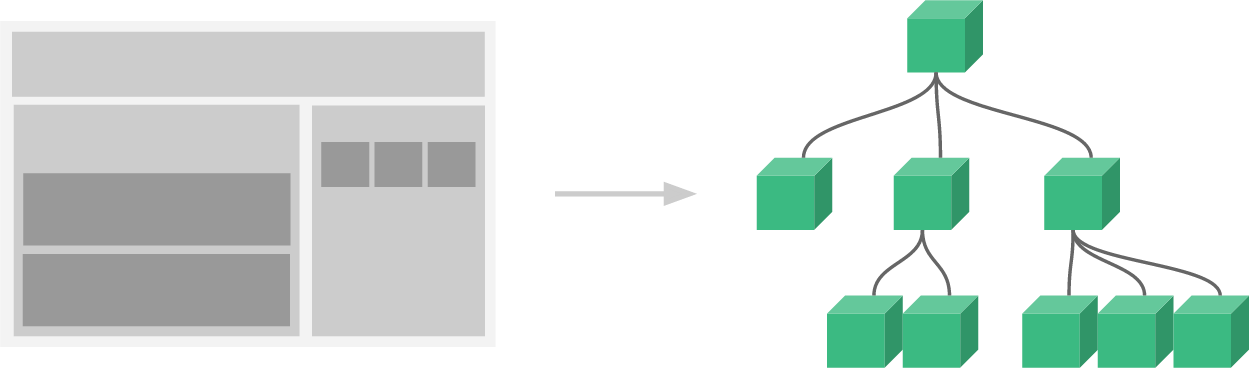
\includegraphics[scale=0.3]{components.png}
\caption{Vue.js组件系统}
\end{figure}


Vue组件可以扩展 HTML 元素,并封装可重用的代码。

\begin{compactitem}
\item 在较高层面上,组件是自定义元素, Vue.js 的编译器为它添加特殊功能。
\item 在有些情况下,组件也可以以 is 特性扩展为原生 HTML 元素的形式。
\end{compactitem}

Vue.js支持在注册组件(或者 props)时使用 kebab-case、camelCase或TitleCase等命名方式。




\begin{lstlisting}[language=JavaScript]
// 在组件定义中
components: {
  // 使用 kebab-case 形式注册
  'kebab-cased-component': { /* ... */ },
  // register using camelCase
  'camelCasedComponent': { /* ... */ },
  // register using TitleCase
  'TitleCasedComponent': { /* ... */ }
}
\end{lstlisting}

\begin{compactitem}
\item 在 HTML 模版中,推荐使用 kebab-case 形式:

\begin{lstlisting}[language=JavaScript]
<!-- 在HTML模版中始终使用 kebab-case -->
<kebab-cased-component></kebab-cased-component>
<camel-cased-component></camel-cased-component>
<title-cased-component></title-cased-component>
\end{lstlisting}

\item 当使用字符串模式时,可以不受 HTML 的 case-insensitive 限制,在模版中可以使用 camelCase 、 TitleCase 或者 kebab-case 来引用:

\begin{lstlisting}[language=JavaScript]
<!-- 在字符串模版中可以用任何你喜欢的方式! -->
<my-component></my-component>
<myComponent></myComponent>
<MyComponent></MyComponent>
\end{lstlisting}

\end{compactitem}

如果组件未经 slot 元素传递内容,Vue.js允许在组件名后使用/使其自闭合:



\begin{lstlisting}[language=JavaScript]
<my-component/>
\end{lstlisting}

自闭合只在字符串模版中有效。因为自闭的自定义元素是无效的 HTML ,浏览器原生的解析器也无法识别它。

\begin{lstlisting}[language=JavaScript]

\end{lstlisting}

\section{Register Component}

Vue支持注册全局组件和局部组件等。

注册一个Vue全局组件语法格式如下:




\begin{lstlisting}[language=JavaScript]
Vue.component(tagName,
   options
)
\end{lstlisting}

其中,tagName是组件名,options是配置选项。

在注册了一个Vue全局组件之后就可以使用如下的方式来调用:


\begin{lstlisting}[language=JavaScript]
<tagName></tagName>
\end{lstlisting}

Vue.js 不强制要求自定义标签名tagName遵循W3C规则 (小写并且包含一个短杠)。



\subsection{Global Component}


默认情况下,全局Vue组件可以通过以下方式注册和创建 :


\begin{lstlisting}[language=JavaScript]
new Vue({
  el: '#some-element',
  // 选项
})
\end{lstlisting}


所有的Vue实例都可以使用全局组件。

\begin{lstlisting}[language=JavaScript]
<div id="app">
    <runoob></runoob>
</div>
 
<script>
// 注册全局组件
Vue.component('runoob', {
  template: '<h1>自定义组件!</h1>'
})
// 创建根实例
new Vue({
  el: '#app'
})
</script>
\end{lstlisting}

\begin{compactenum}
\item 注册全局组件(例如runoob)
\item 创建Vue实例(例如app)
\end{compactenum}










\subsection{Partial Component}

除了在全局注册Vue组件,也可以使用组件实例选项注册局部组件。

Vue局部组件仅在另一个实例/组件的内部作用域中可用,例如:


\begin{lstlisting}[language=JavaScript]
var Child = {
  template: '<div>A custom component!</div>'
}
new Vue({
  // ...
  components: {
    // <my-component> 将只在父模板可用
    'my-component': Child
  }
})
\end{lstlisting}

这种封装也适用于其它可注册的 Vue 功能(如指令)。

\begin{lstlisting}[language=JavaScript]
<div id="app">
    <runoob></runoob>
</div>
 
<script>
var Child = {
  template: '<h1>自定义组件!</h1>'
}
 
// 创建根实例
new Vue({
  el: '#app',
  components: {
    // <runoob> 将只在父模板可用
    'runoob': Child
  }
})
</script>
\end{lstlisting}

\section{Custom Component}

要注册一个全局组件,可以使用 \texttt{Vue.component(tagName, options)}的语法,例如:

\begin{lstlisting}[language=JavaScript]
Vue.component('my-component', {
  // 选项
})
\end{lstlisting}


Vue组件在注册之后就可以在父实例的模块中以自定义元素 <my-component></my-component> 的形式使用,只要确保在初始化根实例 之前 注册了组件即可:


\begin{lstlisting}[language=JavaScript]
<div id="example">
  <my-component></my-component>
</div>

<script>
// 注册组件
Vue.component('my-component', {
  template: '<div>A custom component!</div>'
})
// 创建根实例
new Vue({
  el: '#example'
})
</script>
\end{lstlisting}

最终渲染为:

\begin{lstlisting}[language=JavaScript]
<div id="example">
  <div>A custom component!</div>
</div>
\end{lstlisting}




\begin{lstlisting}[language=JavaScript]

\end{lstlisting}




\begin{lstlisting}[language=JavaScript]

\end{lstlisting}



\section{Component Template}


当使用 DOM 作为组件的模版时(例如将 el 选项挂载到一个已存在的元素上), Vue会受到 HTML 的一些限制,因为 Vue 只有在浏览器解析和标准化 HTML 后才能获取模版内容。

尤其像 <ul>、 <ol>、<table>和<select>等元素限制了能被它包裹的元素, <option> 只能出现在其它元素内部。


在自定义组件中使用上述这些受限制的元素时会导致一些问题,例如:

\begin{lstlisting}[language=JavaScript]
<table>
  <my-row>...</my-row>
</table>
\end{lstlisting}

这里,自定义组件 <my-row> 将会被认为是无效的内容,因此在渲染的时候会导致错误,Vue.js提供的变通的方案是使用特殊的 is 属性:

\begin{lstlisting}[language=JavaScript]
<table>
  <tr is="my-row"></tr>
</table>
\end{lstlisting}

注意,如果使用来自以下来源之一的字符串模板,这些限制将不适用,因此推荐使用字符串模版。

\begin{compactitem}
\item \texttt{<script type="text/x-template">}
\item JavaScript内联模版字符串
\item .vue 组件
\end{compactitem}

HTML 特性不区分大小写,当在Vue组件中使用非字符串模版时,prop的名字形式会从 camelCase 转换为 kebab-case(短横线隔开):

\begin{compactitem}
\item camelCase形式的props

\begin{lstlisting}[language=JavaScript]
Vue.component('child', {
  // camelCase in JavaScript
  props: ['myMessage'],
  template: '<span>{{ myMessage }}</span>'
})
\end{lstlisting}

\item kebab-case形式的props

\begin{lstlisting}[language=JavaScript]
<!-- kebab-case in HTML -->
<child my-message="hello!"></child>
\end{lstlisting}


\end{compactitem}


实际上,如果使用字符串模版,不用在意这些限制。


\subsection{Inline Template}



如果子组件有 inline-template 特性,组件将把它的内容当作它的模板,而不是把它当作分发内容,可以让模板更灵活。

\begin{lstlisting}[language=JavaScript]
<my-component inline-template>
  <div>
    <p>These are compiled as the component's own template.</p>
    <p>Not parent's transclusion content.</p>
  </div>
</my-component>
\end{lstlisting}

不过,inline-template语法让模板的作用域难以理解,Vue.js推荐的最佳实践是使用 template 选项在组件内定义模板或者在 .vue 文件中使用 template 元素。


\subsection{X-Template}


另一种定义模版的方式是在 JavaScript 标签里使用 text/x-template 类型,并且指定一个id。例如:


\begin{lstlisting}[language=JavaScript]
<script type="text/x-template" id="hello-world-template">
  <p>Hello hello hello</p>
</script>
\end{lstlisting}


X-Template在有很多模版或者小的应用中有用,否则应该避免使用,因为它将模版和组件的其他定义隔离了。

\begin{lstlisting}[language=JavaScript]
Vue.component('hello-world', {
  template: '#hello-world-template'
})
\end{lstlisting}





\begin{lstlisting}[language=JavaScript]

\end{lstlisting}






\section{Component Composing}

组件意味着协同工作,通常父子组件的关系就是组件 A 在它的模版中使用了组件 B ,它们之间必然需要相互通信——父组件要给子组件传递数据,子组件需要将它内部发生的事情告知给父组件。

在一个良好定义的接口中尽可能将父子组件解耦是很重要的,这样保证了每个组件可以在相对隔离的环境中书写和理解,最终也大幅提高了组件的可维护性和可重用性。

在 Vue.js 中,父子组件的关系可以总结为 props down, events up:

\begin{compactitem}
\item 父组件通过 props 向下传递数据给子组件;
\item 子组件通过 events 给父组件发送消息。
\end{compactitem}

\begin{figure}[htbp]
\centering
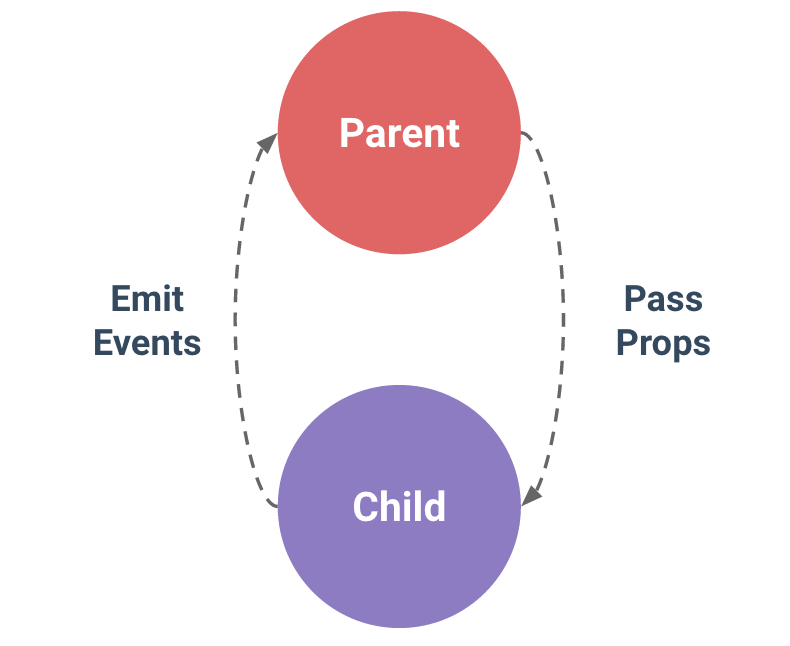
\includegraphics[scale=0.4]{props-events.png}
\caption{Vue.js的父子组件关系}
\end{figure}



props用于从父组件向子组件传递数据。

组件实例的作用域是孤立的,这意味着不能并且不应该在子组件的模板内直接引用父组件的数据,可以使用 props 把数据传给子组件。

prop 是父组件用来传递数据的一个自定义属性,子组件需要显式地用 props 选项声明 “prop”:

\begin{lstlisting}[language=JavaScript]
Vue.component('child',{
  // 声明props
  props: ['message'],
  // prop和data都可以用在模板内
  // 同样就可以在vm实例中使用this.message来访问
  template: '<span>{{ message }}</span>'
})
\end{lstlisting}

向Vue组件中传入一个普通字符串并检查结果:


\begin{lstlisting}[language=JavaScript]
<child message="hello!"></child>
\end{lstlisting}

下面是一个使用prop传递数据的示例:

\begin{lstlisting}[language=JavaScript]
<div id="prop-example-1">
  <child></child>
</div>

<script>
new Vue({
  el: '#prop-example-1',
  components: {
     child: {
        props: ['message'],
        template: '<span>{{ message }}</span>'
     }
  }
})
</script>
\end{lstlisting}



最终渲染结果如下:


\begin{lstlisting}[language=JavaScript]
<div id="prop-example-1" class="demo">
  <span>hello!</span>
</div>
\end{lstlisting}


\subsection{Child Component}

尽管有 props 和 events ,但是有时仍然需要在 JavaScript 中直接访问子组件,为此可以使用 ref 为子组件指定一个索引 ID 。例如:





\begin{lstlisting}[language=JavaScript]
<div id="parent">
  <user-profile ref="profile"></user-profile>
</div>
\end{lstlisting}



\begin{lstlisting}[language=JavaScript]
var parent=new Vue({el: '#parent'})
// 访问子组件
var child = parent.$refs.profile
\end{lstlisting}

当 ref 和 v-for 一起使用时, ref 是一个数组或对象,包含相应的子组件。

注意,\$refs 只在组件渲染完成后才填充,并且它是非响应式的。它仅仅作为一个直接访问子组件的应急方案——应当避免在模版或计算属性中使用 \$refs 。


\subsection{Async Component}


在大型应用中可能需要将应用拆分为多个小模块,按需从服务器下载。

为了简化模块拆分, Vue.js 允许将组件定义为一个工厂函数,动态地解析组件的定义。

Vue.js 只在组件需要渲染时触发工厂函数,并且把结果缓存起来,用于后面的再次渲染。例如:

\begin{lstlisting}[language=JavaScript]
Vue.component('async-example',function(resolve,reject){
   setTimeout(function(){
      // pass the component definition to the resolve callback
      resolve({
         template: '<div>I am async!</div>'
      })
   },1000)
})
\end{lstlisting}

工厂函数接收一个 resolve 回调,在收到从服务器下载的组件定义时调用,也可以调用 reject(reason) 指示加载失败。这里 setTimeout 只是为了演示,具体图和获取组件可以完全自定义,或者配合Webpack的代码分割功能使用。



\begin{lstlisting}[language=JavaScript]
Vue.component('async-webpack-example', function (resolve) {
  // 这个特殊的 require 语法告诉 webpack
  // 自动将编译后的代码分割成不同的块,
  // 这些块将通过 Ajax 请求自动下载。
  require(['./my-async-component'], resolve)
})
\end{lstlisting}

可以使用 Webpack 2 + ES2015 的语法返回一个 Promise resolve 函数:


\begin{lstlisting}[language=JavaScript]
Vue.component(
  'async-webpack-example',
  () => System.import('./my-async-component')
)
\end{lstlisting}

Browserify不支持异步加载,因此Browserify无法使用异步组件,Webpack则提供了一流的异步支持。

\subsection{Recursive Component}

组件在它的模板内可以递归地调用自己,不过,只有当它有 name 选项时才可以:

\begin{lstlisting}[language=JavaScript]
name: 'unique-name-of-my-component'
\end{lstlisting}

当使用Vue.component在全局注册了一个组件后,全局组件的ID会作为组件的 name 选项被自动设置。



\begin{lstlisting}[language=JavaScript]
Vue.component('unique-name-of-my-component', {
  // ...
})
\end{lstlisting}

如果使用不当,递归组件可能导致死循环,例如下面的组件会导致一个错误 “max stack size exceeded” ,所以要确保递归调用有终止条件 (比如递归调用时使用 v-if 并让他最终返回 false )。


\begin{lstlisting}[language=JavaScript]
name: 'stack-overflow',
template: '<div><stack-overflow></stack-overflow></div>'
\end{lstlisting}



\subsection{Circular Reference}

如果需要创建一个文件目录树,那么可以使用下面的模板来创建一个tree-folder组件:


\begin{lstlisting}[language=JavaScript]
<p>
  <span>{{ folder.name }}</span>
  <tree-folder-contents :children="folder.children"/>
</p>
\end{lstlisting}

其中,tree-folder-contents组件使用下面的模板来创建:

\begin{lstlisting}[language=JavaScript]
<ul>
  <li v-for="child in children">
    <tree-folder v-if="child.children" :folder="child"/>
    <span v-else>{{ child.name }}</span>
  </li>
</ul>
\end{lstlisting}

在渲染树上,这些组件实际上是彼此的后代和祖先——这是一个悖论,当使用Vue.component在全局注册组件时,这个矛盾是自动解决的。

如果使用模块系统(例如Webpack或Browserify)来引用/导入组件,将会得到一个错误:


\begin{lstlisting}[language=JavaScript]
Failed to mount component: template or render function not defined.
\end{lstlisting}

为了解释发生了什么,这里以组件A和B为例进行解释,模块系统需要A,但是A需要B,同时B需要A,这样Webpack或Browserify就被困在一个循环中, 不知道如何完全解析任何一个组件,而不先解析另一个。 

为了要解决上述这个问题,我们需要给模块系统一个点,它可以说,“A最终需要B,但是没有必要先解析B”。

在tree-folder的例子中,引发矛盾的地方是tree-folder-contents组件,所以可以等到beforeCreate生命周期钩子中再注册它就可以解决这个问题。


\begin{lstlisting}[language=JavaScript]
beforeCreate: function () {
  this.$options.components.TreeFolderContents = require('./tree-folder-contents.vue')
}
\end{lstlisting}


\begin{lstlisting}[language=JavaScript]

\end{lstlisting}




\begin{lstlisting}[language=JavaScript]

\end{lstlisting}


\section{Dynamic Component}


多个组件可以使用同一个挂载点,然后动态地在它们之间切换。

\begin{lstlisting}[language=JavaScript]
var vm = new Vue({
  el: '#example',
  data: {
    currentView: 'home'
  },
  components: {
    home: { /* ... */ },
    posts: { /* ... */ },
    archive: { /* ... */ }
  }
})
\end{lstlisting}


使用保留的 <component> 元素,动态地绑定到它的 is 特性:


\begin{lstlisting}[language=JavaScript]
<component v-bind:is="currentView">
  <!-- 组件在 vm.currentview 变化时改变! -->
</component>
\end{lstlisting}

也可以直接绑定到组件对象上:

\begin{lstlisting}[language=JavaScript]
var Home = {
  template: '<p>Welcome home!</p>'
}
var vm = new Vue({
  el: '#example',
  data: {
    currentView: Home
  }
})
\end{lstlisting}



\begin{lstlisting}[language=JavaScript]

\end{lstlisting}



\begin{lstlisting}[language=JavaScript]

\end{lstlisting}




\begin{lstlisting}[language=JavaScript]

\end{lstlisting}



\begin{lstlisting}[language=JavaScript]

\end{lstlisting}




\section{Memery Component}


如果把切换出去的组件保留在内存中,可以保留它的状态或避免重新渲染。为此可以添加一个 keep-alive 指令参数:

\begin{lstlisting}[language=JavaScript]
<keep-alive>
  <component :is="currentView">
    <!-- 非活动组件将被缓存! -->
  </component>
</keep-alive>
\end{lstlisting}


\section{Reusable Component}

一次性组件跟其它组件紧密耦合没关系,可复用组件应当定义一个清晰的公开接口。

Vue 组件的 API 来自三部分 - props, events 和 slots :

\begin{compactitem}
\item Props允许外部环境传递数据给组件
\item Events允许组件触发外部环境的副作用
\item Slots允许外部环境将额外的内容组合在组件中
\end{compactitem}

使用 v-bind 和 v-on 的简写语法,模板的缩进清楚且简洁:


\begin{lstlisting}[language=JavaScript]
<my-component
  :foo="baz"
  :bar="qux"
  @event-a="doThis"
  @event-b="doThat"
>
  <img slot="icon" src="...">
  <p slot="main-text">Hello!</p>
</my-component>
\end{lstlisting}

\section{Static Component}


尽管在 Vue 中渲染 HTML 很快,不过当组件中包含大量静态内容时,可以考虑使用 v-once的低级静态组件(cheap static component)将渲染结果缓存起来。



\begin{lstlisting}[language=JavaScript]
Vue.component('terms-of-service', {
  template: '\
    <div v-once>\
      <h1>Terms of Service</h1>\
      ... a lot of static content ...\
    </div>\
  '
})
\end{lstlisting}



\begin{lstlisting}[language=JavaScript]

\end{lstlisting}




\begin{lstlisting}[language=JavaScript]

\end{lstlisting}



\begin{lstlisting}[language=JavaScript]

\end{lstlisting}




\begin{lstlisting}[language=JavaScript]

\end{lstlisting}



\begin{lstlisting}[language=JavaScript]

\end{lstlisting}







\chapter{Vue Event Handler}

Vue的事件监听的方式违背了关注点分离(separation of concern)传统理念。不必担心,因为所有的 Vue.js 事件处理方法和表达式都严格绑定在当前视图的 ViewModel 上,它不会导致任何维护上的困难。实际上,使用 v-on 有几个好处:

\begin{compactitem}
\item 在HTML模板中可以轻松定位在 JavaScript 代码里对应的方法。

\item 无须在 JavaScript 里手动绑定事件,ViewModel 代码可以是非常纯粹的逻辑,和 DOM 完全解耦,更易于测试。
\item 当一个 ViewModel 被销毁时,所有的事件处理器都会自动被删除,无须担心如何自己清理它们。
\end{compactitem}

可以用 v-on 指令监听 DOM 事件来触发一些 JavaScript 代码。


\begin{lstlisting}[language=JavaScript]
<div id="example-1">
  <button v-on:click="counter += 1">增加 1</button>
  <p>这个按钮被点击了 {{ counter }} 次。</p>
</div>

<script>
var example1=new Vue({
  el: '#example-1',
  data: {
     counter: 0
  }
})
</script>
\end{lstlisting}



\begin{lstlisting}[language=JavaScript]

\end{lstlisting}



\begin{lstlisting}[language=JavaScript]

\end{lstlisting}

\section{Event Handler}

许多事件处理的逻辑都很复杂,所以直接把 JavaScript 代码写在 v-on 指令中是不可行的,因此 v-on 可以接收一个定义的方法来调用。

\begin{lstlisting}[language=JavaScript]
<div id="example-2">
  <!-- `greet` 是在下面定义的方法名 -->
  <button v-on:click="greet">Greet</button>
</div>

<script>
var example2 = new Vue({
  el: '#example-2',
  data: {
    name: 'Vue.js'
  },
  // 在 `methods` 对象中定义方法
  methods: {
    greet: function (event) {
      // `this` 在方法里指当前 Vue 实例
      alert('Hello ' + this.name + '!')
      // `event` 是原生 DOM 事件
      alert(event.target.tagName)
    }
  }
})
// 也可以用 JavaScript 直接调用方法
example2.greet() // -> 'Hello Vue.js!'
</script>
\end{lstlisting}



\begin{lstlisting}[language=JavaScript]

\end{lstlisting}



\begin{lstlisting}[language=JavaScript]

\end{lstlisting}


\section{Inline Handler}

除了直接绑定到一个方法,也可以用内联 JavaScript 语句:

\begin{lstlisting}[language=JavaScript]
<div id="example-3">
  <button v-on:click="say('hi')">Say hi</button>
  <button v-on:click="say('what')">Say what</button>
</div>

<script>
new Vue({
  el: '#example-3',
  methods: {
    say: function (message) {
      alert(message)
    }
  }
})
</script>
\end{lstlisting}

有时也需要在内联语句处理器中访问原生 DOM 事件,可以用特殊变量 \$event 把它传入方法:

\begin{lstlisting}[language=JavaScript]
<button v-on:click="warn('Form cannot be submitted yet.', $event)">Submit</button>

<script>
// ...
methods: {
  warn: function (message, event) {
    // 现在我们可以访问原生事件对象
    if (event) event.preventDefault()
    alert(message)
  }
}
</script>
\end{lstlisting}



\begin{lstlisting}[language=JavaScript]

\end{lstlisting}


\section{Event Modifier}


在事件处理程序中调用 event.preventDefault() 或 event.stopPropagation() 是非常常见的需求。尽管我们可以在 methods 中轻松实现这点,但更好的方式是:methods 只有纯粹的数据逻辑,而不是去处理 DOM 事件细节。

为了解决这个问题, Vue.js 为 v-on 提供了 事件修饰符。通过由点(.)表示的指令后缀来调用修饰符。

\subsection{.stop}

\begin{lstlisting}[language=JavaScript]
<!-- 阻止单击事件冒泡 -->
<a v-on:click.stop="doThis"></a>
\end{lstlisting}

\subsection{.prevent}

\begin{lstlisting}[language=JavaScript]
<!-- 提交事件不再重载页面 -->
<form v-on:submit.prevent="onSubmit"></form>
\end{lstlisting}


\begin{lstlisting}[language=JavaScript]
<!-- 修饰符可以串联  -->
<a v-on:click.stop.prevent="doThat"></a>
\end{lstlisting}

\begin{lstlisting}[language=JavaScript]
<!-- 只有修饰符 -->
<form v-on:submit.prevent></form>
\end{lstlisting}



\subsection{.capture}


\begin{lstlisting}[language=JavaScript]
<!-- 添加事件侦听器时使用事件捕获模式 -->
<div v-on:click.capture="doThis">...</div>
\end{lstlisting}

\subsection{.self}

\begin{lstlisting}[language=JavaScript]
<!-- 只当事件在该元素本身(而不是子元素)触发时触发回调 -->
<div v-on:click.self="doThat">...</div>
\end{lstlisting}

\subsection{.once}

\begin{lstlisting}[language=JavaScript]
<!-- the click event will be triggered at most once -->
<a v-on:click.once="doThis"></a>
\end{lstlisting}




Unlike the other modifiers, which are exclusive to native DOM events, the .once modifier can also be used on component events. If you haven’t read about components yet, don’t worry about this for now.








\section{Key Modifier}



在监听键盘事件时,我们经常需要监测常见的键值。 Vue 允许为 v-on 在监听键盘事件时添加按键修饰符:



\begin{lstlisting}[language=JavaScript]
<!-- 只有在 keyCode 是 13 时调用 vm.submit() -->
<input v-on:keyup.13="submit">
\end{lstlisting}

 Vue 为最常用的按键提供了别名:

\begin{lstlisting}[language=JavaScript]
<!-- 同上 -->
<input v-on:keyup.enter="submit">
<!-- 缩写语法 -->
<input @keyup.enter="submit">
\end{lstlisting}

全部的按键别名如下:

\begin{compactitem}
\item .enter
\item .tab
\item .delete (捕获 “删除” 和 “退格” 键)
\item .esc
\item .space
\item .up
\item .down
\item .left
\item .right
\end{compactitem}

可以通过全局 config.keyCodes 对象自定义按键修饰符别名:

\begin{lstlisting}[language=JavaScript]
// 可以使用 v-on:keyup.f1
Vue.config.keyCodes.f1 = 112
\end{lstlisting}







\section{Modifier Key}


可以用如下修饰符开启鼠标或键盘事件监听,使在按键按下时发生响应。


\begin{compactitem}
\item .ctrl
\item .alt
\item .shift
\item .meta
\end{compactitem}

On Macintosh keyboards, meta is the command key (⌘). On Windows keyboards, meta is the windows key (⊞). On Sun Microsystems keyboards, meta is marked as a solid diamond (◆). On certain keyboards, specifically MIT and Lisp machine keyboards and successors, such as the Knight keyboard, space-cadet keyboard, meta is labeled “META”. On Symbolics keyboards, meta is labeled “META” or “Meta”.

\begin{lstlisting}[language=JavaScript]
<!-- Alt + C -->
<input @keyup.alt.67="clear">
<!-- Ctrl + Click -->
<div @click.ctrl="doSomething">Do something</div>
\end{lstlisting}


\begin{lstlisting}[language=JavaScript]

\end{lstlisting}



\begin{lstlisting}[language=JavaScript]

\end{lstlisting}

\part{Vue NPM}



\section{Node}


\begin{lstlisting}[language=bash]
$ curl -sL https://deb.nodesource.com/setup_7.x | sudo -E bash -
$ sudo apt-get install -y nodejs
$ node -v
v7.5.0
$ nodejs -v
v7.5.0
$ npm -v
4.1.2
\end{lstlisting}


\section{NPM}

\begin{lstlisting}[language=bash]
$ npm install -g npm@latest
$ npm -v
4.1.2
\end{lstlisting}

进入/path/to/hitour/themes/kitchen安装项目依赖:


\begin{lstlisting}[language=bash]
$ cd /path/to/hitour/themes/kitchen
$ sudo npm i
\end{lstlisting}

\begin{figure}[htbp]
\centering
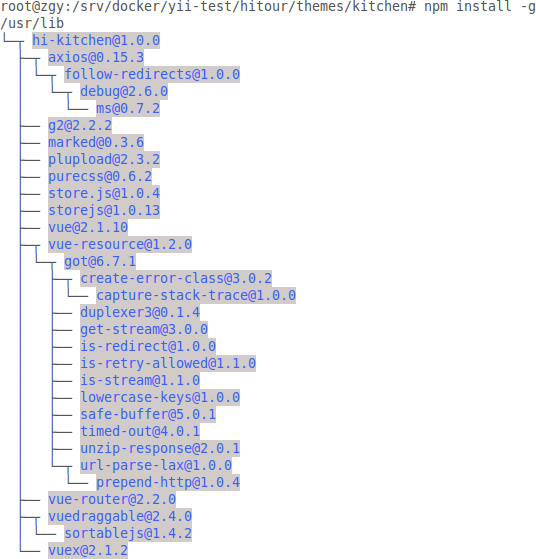
\includegraphics[scale=0.4]{kitchen-dependence.png}
\caption{kitchen项目前端依赖关系}
\end{figure}


创建本地的前端开发服务器配置文件/path/to/hitour/themes/kitchen/config/index.js,index.js的内容如下:

\begin{lstlisting}[language=JavaScript]
var path = require('path')

var common_proxy = {
  //target       : 'http://test.hitour.cc',
  //target       : 'http://sandbox.hitour.cc',
  target: 'http://trial.hitour.cc',
  // target       : 'http://hitour.host',
  changeOrigin: true,
  pathRewrite: {}
};

module.exports = {
  build: {
    env: require('./prod.env'),
    index: path.resolve(__dirname, '../dist/index.html'),
    assetsRoot: path.resolve(__dirname, '../dist'),
    assetsSubDirectory: 'static',
    assetsPublicPath: '/themes/kitchen/dist/',
    productionSourceMap: true,
    productionGzip: false,
    productionGzipExtensions: ['js', 'css']
  },
  dev: {
    env: require('./dev.env'),
    port: 60003,
    assetsSubDirectory: 'static',
    assetsPublicPath: '/',
    proxyTable: {
      '/admin/': common_proxy,
      '/chef/': common_proxy,
      '/themes': common_proxy,
      '/markMi/': common_proxy
    },
    cssSourceMap: false
  }
}
\end{lstlisting}

在/path/to/hitour/themes/kitchen目录下启动本地测试服务器,并且在\url{http://localhost:10003/k/sign\_in}进行测试。

\begin{lstlisting}[language=bash]
$ cd /path/to/hitour/themes/kitchen
$ npm run dev
\end{lstlisting}

如果本地测试通过,可以执行\texttt{npm run build}进行发布。

\begin{lstlisting}[language=bash]
$ cd /path/to/hitour/themes/kitchen
$ npm run build
\end{lstlisting}

注意,在本地或远程服务器做发布之前, 需要确认Yii的路由配置。

\subsection{access}

\begin{lstlisting}[language=bash]

\end{lstlisting}

\subsection{adduser}

\begin{lstlisting}[language=bash]

\end{lstlisting}

\subsection{bin}


\begin{lstlisting}[language=bash]

\end{lstlisting}

\subsection{bugs}


\begin{lstlisting}[language=bash]

\end{lstlisting}

\subsection{c}



\begin{lstlisting}[language=bash]

\end{lstlisting}

\subsection{cache}


\begin{lstlisting}[language=bash]

\end{lstlisting}

\subsection{completion}



\begin{lstlisting}[language=bash]

\end{lstlisting}

\subsection{config}


\begin{lstlisting}[language=bash]
$ npm config list

\end{lstlisting}

\subsection{ddp}


\begin{lstlisting}[language=bash]

\end{lstlisting}

\subsection{dedupe}



\begin{lstlisting}[language=bash]

\end{lstlisting}

\subsection{deprecate}




\begin{lstlisting}[language=bash]

\end{lstlisting}

\subsection{dist-tag}


\begin{lstlisting}[language=bash]

\end{lstlisting}

\subsection{docs}



\begin{lstlisting}[language=bash]
$ npm docs vue
\end{lstlisting}



\begin{lstlisting}[language=bash]
$ npm docs webpack
\end{lstlisting}


\begin{lstlisting}[language=bash]

\end{lstlisting}



\begin{lstlisting}[language=bash]

\end{lstlisting}

\subsection{doctor}



\begin{lstlisting}[language=bash]

\end{lstlisting}

\subsection{edit}



\begin{lstlisting}[language=bash]

\end{lstlisting}

\subsection{explore}



\begin{lstlisting}[language=bash]

\end{lstlisting}

\subsection{get}



\begin{lstlisting}[language=bash]

\end{lstlisting}

\subsection{help}



\begin{lstlisting}[language=bash]

\end{lstlisting}

\subsection{help-search}

\begin{lstlisting}[language=bash]

\end{lstlisting}

\subsection{i}


\begin{lstlisting}[language=bash]

\end{lstlisting}

\subsection{init}


\begin{lstlisting}[language=bash]

\end{lstlisting}

\subsection{install}


\begin{lstlisting}[language=bash]

\end{lstlisting}

\subsection{install-test}


\begin{lstlisting}[language=bash]

\end{lstlisting}

\subsection{it}


\begin{lstlisting}[language=bash]

\end{lstlisting}

\subsection{link}


\begin{lstlisting}[language=bash]

\end{lstlisting}

\subsection{list}


\begin{lstlisting}[language=bash]

\end{lstlisting}

\subsection{ln}



\begin{lstlisting}[language=bash]

\end{lstlisting}

\subsection{login}



\begin{lstlisting}[language=bash]

\end{lstlisting}

\subsection{logout}



\begin{lstlisting}[language=bash]

\end{lstlisting}

\subsection{ls}



\begin{lstlisting}[language=bash]

\end{lstlisting}

\subsection{outdated}


\begin{lstlisting}[language=bash]

\end{lstlisting}


\subsection{owner}


\begin{lstlisting}[language=bash]

\end{lstlisting}

\subsection{pack}


\begin{lstlisting}[language=bash]

\end{lstlisting}

\subsection{ping}



\begin{lstlisting}[language=bash]

\end{lstlisting}

\subsection{prefix}


\begin{lstlisting}[language=bash]

\end{lstlisting}

\subsection{prune}

\begin{lstlisting}[language=bash]

\end{lstlisting}

\subsection{publish}


\begin{lstlisting}[language=bash]

\end{lstlisting}

\subsection{rb}



\begin{lstlisting}[language=bash]

\end{lstlisting}

\subsection{rebuild}




\begin{lstlisting}[language=bash]

\end{lstlisting}

\subsection{repo}


\begin{lstlisting}[language=bash]

\end{lstlisting}

\subsection{restart}

\begin{lstlisting}[language=bash]

\end{lstlisting}

\subsection{root}


\begin{lstlisting}[language=bash]

\end{lstlisting}

\subsection{run}



\begin{lstlisting}[language=bash]

\end{lstlisting}

\subsection{run-script}


\begin{lstlisting}[language=bash]

\end{lstlisting}

\subsection{s}


\begin{lstlisting}[language=bash]

\end{lstlisting}


\subsection{se}


\begin{lstlisting}[language=bash]

\end{lstlisting}

\subsection{search}



\begin{lstlisting}[language=bash]

\end{lstlisting}

\subsection{set}



\begin{lstlisting}[language=bash]

\end{lstlisting}

\subsection{shrinkwrap}




\begin{lstlisting}[language=bash]

\end{lstlisting}

\subsection{star}




\begin{lstlisting}[language=bash]

\end{lstlisting}

\subsection{stars}

\begin{lstlisting}[language=bash]

\end{lstlisting}

\subsection{start}


\begin{lstlisting}[language=bash]

\end{lstlisting}

\subsection{stop}



\begin{lstlisting}[language=bash]

\end{lstlisting}


\subsection{t}


\begin{lstlisting}[language=bash]

\end{lstlisting}

\subsection{team}



\begin{lstlisting}[language=bash]

\end{lstlisting}

\subsection{test}




\begin{lstlisting}[language=bash]

\end{lstlisting}

\subsection{tst}






\begin{lstlisting}[language=bash]

\end{lstlisting}

\subsection{un}

\begin{lstlisting}[language=bash]

\end{lstlisting}

\subsection{uninstall}


\begin{lstlisting}[language=bash]

\end{lstlisting}

\subsection{unpublish}



\begin{lstlisting}[language=bash]

\end{lstlisting}

\subsection{unstar}




\begin{lstlisting}[language=bash]

\end{lstlisting}

\subsection{up}



\begin{lstlisting}[language=bash]

\end{lstlisting}

\subsection{update}



\begin{lstlisting}[language=bash]

\end{lstlisting}

\subsection{v}





\begin{lstlisting}[language=bash]

\end{lstlisting}

\subsection{version}

\begin{lstlisting}[language=bash]
$ npm version
{
  npm: '4.1.2',
  ares: '1.10.1-DEV',
  cldr: '29.0',
  http_parser: '2.7.0',
  icu: '57.1',
  modules: '51',
  node: '7.5.0',
  openssl: '1.0.2k',
  tz: '2016b',
  unicode: '8.0',
  uv: '1.10.2',
  v8: '5.4.500.48',
  zlib: '1.2.8' 
}
\end{lstlisting}

\subsection{view}


\begin{lstlisting}[language=bash]
$ npm view vue version
2.1.10
$ npm view vue-cli version
2.8.1
$ npm view vue-router version
2.20
$ npm view vue-resource version
1.2.0
$ npm view webpack version
2.2.1
\end{lstlisting}

\subsection{whoami}



\begin{lstlisting}[language=bash]

\end{lstlisting}




\begin{lstlisting}[language=bash]

\end{lstlisting}




\begin{lstlisting}[language=bash]

\end{lstlisting}




\begin{lstlisting}[language=bash]

\end{lstlisting}



\section{CNPM}

可以使用定制的 cnpm (gzip 压缩支持) 命令行工具代替默认的 npm:

\begin{lstlisting}[language=bash]
$ npm install -g cnpm --registry=https://registry.npm.taobao.org
\end{lstlisting}

或者直接通过添加 npm 参数 alias 一个新命令:

\begin{lstlisting}[language=bash]
$ alias cnpm="npm --registry=https://registry.npm.taobao.org \
--cache=$HOME/.npm/.cache/cnpm \
--disturl=https://npm.taobao.org/dist \
--userconfig=$HOME/.cnpmrc"

# Or alias it in .bashrc or .zshrc
$ echo '\n#alias for cnpm\nalias cnpm="npm --registry=https://registry.npm.taobao.org \
  --cache=$HOME/.npm/.cache/cnpm \
  --disturl=https://npm.taobao.org/dist \
  --userconfig=$HOME/.cnpmrc"' >> ~/.zshrc && source ~/.zshrc
\end{lstlisting}

从 registry.npm.taobao.org 安装模块时,如果发现安装的模块还没有同步过来, 淘宝 NPM 会自动在后台进行同步, 并且会让用户从官方 NPM registry.npmjs.org 进行安装. 下次再安装这个模块的时候, 就会直接从 淘宝 NPM 安装了。


\begin{lstlisting}[language=bash]
$ cnpm install [name]
\end{lstlisting}

直接通过 sync 命令马上同步一个模块, 注意只有 cnpm 命令行才有此功能:

\begin{lstlisting}[language=bash]
$ cnpm sync connect
\end{lstlisting}

可以直接通过 web 方式来同步: /sync/connect

\begin{lstlisting}[language=bash]
$ open https://npm.taobao.org/sync/connect
\end{lstlisting}


cnpm支持 npm 除了 publish 之外的所有命令, 例如:

\begin{lstlisting}[language=bash]
$ cnpm info connect
\end{lstlisting}


\section{Nginx}




\begin{lstlisting}[language=bash]

\end{lstlisting}


\begin{lstlisting}[language=bash]

\end{lstlisting}


\begin{lstlisting}[language=bash]

\end{lstlisting}

\section{Webpack}


\begin{lstlisting}[language=bash]
$ sudo npm i webpack -g
/usr/bin/webpack -> /usr/lib/node_modules/webpack/bin/webpack.js
$ webpack -v
2.2.1
\end{lstlisting}

\part{Vue Config}


\chapter{Overview}


Vue.config 是一个对象,包含 Vue 的全局配置,可以在启动应用之前修改下列属性:


\begin{compactitem}
\item silent:取消 Vue 所有的日志与警告
\item optionMergeStrategies:自定义合并策略的选项
\item devtools:配置是否允许 vue-devtools 检查代码
\item errorHandler:指定组件的渲染和观察期间未捕获错误的处理函数
\item ignoredElements:须使 Vue 忽略在 Vue 之外的自定义元素
\item keyCodes:给 v-on 自定义键位别名
\end{compactitem}


\section{silent}

取消 Vue 所有的日志与警告

\begin{compactitem}
\item 类型:boolean
\item 默认值:false
\end{compactitem}




\begin{lstlisting}[language=JavaScript]
Vue.config.silent = true
\end{lstlisting}


\section{optionMergeStrategies}

自定义合并策略的选项

\begin{compactitem}
\item 类型:\texttt{\{ [key: string]: Function \}}
\item 默认值:\texttt{\{\}}
\end{compactitem}

\begin{lstlisting}[language=JavaScript]
Vue.config.optionMergeStragegies._my_option = function (parent, child, vm) {
   return child  1;
}

const Profile = Vue.extend({
   _my_option: 1
})

// Profile.options._my_option = 2
\end{lstlisting}


合并策略选项分别接受第一个参数作为父实例,第二个参数为子实例,Vue实例上下文被作为第三个参数传入。

\section{devtools}


配置是否允许 vue-devtools 检查代码

\begin{compactitem}
\item 类型:boolean
\item 默认值:true(生产版本为false)
\end{compactitem}



\begin{lstlisting}[language=JavaScript]
// 务必在加载Vue之后,立即同步设置以下内容
Vue.config.devtools = true
\end{lstlisting}

开发版本默认为 true,生产版本默认为 false。生产版本设为 true 可以启用检查。


\section{errorHandler}

指定组件的渲染和观察期间未捕获错误的处理函数

\begin{compactitem}
\item 类型:Function
\item 默认值:默认抛出异常
\end{compactitem}



\begin{lstlisting}[language=JavaScript]
Vue.config.errorHandler = function (err, vm) {
   // handle error
}
\end{lstlisting}

这个处理函数被调用时,可获取错误信息和 Vue 实例。



\section{ignoredElements}

须使 Vue 忽略在 Vue 之外的自定义元素(e.g., 使用了 Web Components APIs),否则,它会假设你忘记注册全局组件或者拼错了组件名称,从而抛出一个关于 Unknown custom element 的警告。

\begin{compactitem}
\item 类型:Array<string>
\item 默认值:[]
\end{compactitem}

\begin{lstlisting}[language=JavaScript]
Vue.config.ignoredElements = [
   'my-custom-web-component',
   'another-web-component'
]
\end{lstlisting}



\section{keyCodes}


给 v-on 自定义键位别名

\begin{compactitem}
\item 类型:\texttt{ \{[key: string]: number | Array<number>\} }
\item 默认值:\texttt{\{ \}}
\end{compactitem}



\begin{lstlisting}[language=JavaScript]
Vue.config.keyCodes = {
  v: 86,
  f1: 112,
  mediaPlayPause: 179,
  up: [38, 87]
}
\end{lstlisting}




\part{Vue Binding}


\chapter{Overview}

数据绑定就是把数据和视图进行关联,当数据发生变化时可以自动更新视图。Vue.js把数据绑定的语法设计为可配置的,可以在Vue.config全局配置上修改数据绑定的语法。



\begin{lstlisting}[language=JavaScript]
let delimiters = ['{{','}}']
let unsafeDelimiters = ['{{{','}}}']
\end{lstlisting}

Vue.config是一个包含了Vue.js所有的全局配置的对象,可以在Vue.js实例化之前修改其中的属性。



\begin{lstlisting}[language=JavaScript]
Vue.config.delimeters = ['<%','%>]
Vue.config.unsafeDelimeters = ['<$','$>']
\end{lstlisting}

不同的JavaScript框架都提供了自己的数据绑定语法,Vue.js提供了不同的文本渲染方式来满足日常的模板渲染需求。




数据绑定一个常见需求是操作元素的 class 列表和它的内联样式,class和style都是属性 ,可以用v-bind 处理它们——只需要计算出表达式最终的字符串。

不过,字符串拼接麻烦又易错,在 v-bind 用于 class 和 style 时, Vue.js 专门增强了它,现在表达式的结果类型除了字符串之外,还可以是对象或数组。

\section{Mustache}

Vue.js支持使用Mustache标签(也就是双大括号\{\{\}\})来来处理文本插值。


\begin{lstlisting}[language=JavaScript]
<span>Text: {{ text }}</span>
\end{lstlisting}

上述的标签\{\{text\}\}被相应的数据对象的text属性的值替换,而且当text的值改变时,文本中的值也会联动地发生变化。

如果数据只需要渲染一次,后续不再更新,可以使用\texttt{"*"}来进行指定:

\begin{lstlisting}[language=JavaScript]
<span>{{ *text }}</span>
\end{lstlisting}

默认情况下,\{\{\}\}会把内部的值全部作为字符串进行处理,如果值是HTML片段,可以使用三个大括号来绑定,例如:


\begin{lstlisting}[language=JavaScript]
<div>Logo: {{{ logo }}}</div>

logo: '<span>Hello</span>'
\end{lstlisting}

Vue.js支持把\{\{\}\}放在HTML标签内,例如:

\begin{lstlisting}[language=JavaScript]
<li data-id='{{ id }}'></li>
\end{lstlisting}


注意,Vue.js指令和自身特性内是不可以插值的,否则Vue.js会发出警告。


文本插值支持字符串、HTML片段以及表达式形式的值,表达式可以由JavaScript表达式和过滤器构成,而且过滤器可以没有,也可以有多个。

复杂的JavaScript表达式可以是数值、变量和运算符的综合体,简单的JavaScript表达式可以是常量或变量名称,表达式的值是其运算结果。



\begin{lstlisting}[language=JavaScript]
{{ cents/10 }}
{{ true ? 1 : 0 }}
{{ example.split(' ') }}
\end{lstlisting}

下面的插值是不合法的:

\begin{lstlisting}[language=JavaScript]
{{ var logo = 'hello' }} // 语句不是表达式
{{ if(true) return 'world' }} // 只支持三元式,不支持条件控制语句
\end{lstlisting}

Vue.js支持在表达式后面添加过滤符来实现类似Linux中的管道的功能的过滤器,例如:


\begin{lstlisting}[language=JavaScript]
{{ example | toUpperCase }}
\end{lstlisting}

JavaScript过滤器本质上是一个JavaScript函数,而且Vue.js允许串联过滤器。

\begin{lstlisting}[language=JavaScript]
{{ example | filterA | filterB }}
\end{lstlisting}

Vue.js支持带有参数的过滤器,参数之间使用空格隔开,例如:


\begin{lstlisting}[language=JavaScript]
{{ example | filter a b }}
\end{lstlisting}

Vue.js提供了一些内置的过滤器。

\section{Directive}


Vue.js提供的指令可以理解为带有v-前缀的特殊特性,指令的值限定为绑定表达式,即JavaScript表达式和过滤器。

Vue.js指令的职责就是当表达式的值发生变化时,联动地把某些特殊的行为反映到DOM上来实现视图更新,例如:


\begin{lstlisting}[language=JavaScript]
<div v-if="show">Hello</div>
\end{lstlisting}


这里,如果show为true则显示Hello,否则就不显示。

Vue.js还支持在指令和表达式之间插入一个用冒号分隔的参数,例如:

\begin{lstlisting}[language=JavaScript]
<a v-bind:href="url"></a>
<div v-on:click="action"></div>
\end{lstlisting}

Vue.js提供了一些内置的指令,例如:

\begin{compactitem}
\item v-el
\item v-on
\item v-bind
\item v-cloak
\item v-if
\item v-else
\item v-show
\item v-for
\item v-repeat
\item v-model
\item v-text
\item v-html
\item v-ref
\item v-pre
\end{compactitem}

\subsection{v-if}


\section{Binding HTML Classes}



\subsection{Object Syntax}

可以传给\texttt{v-bind:class} 一个对象来动态地切换 class 。

\begin{lstlisting}[language=JavaScript]
<div v-bind:class="{ active: isActive }"></div>
\end{lstlisting}

上面的语法表示 class~active 的更新将取决于数据属性 isActive 是否为真值 。

也可以在对象中传入更多属性用来动态切换多个 class 。

此外, \texttt{v-bind:class}指令可以与普通的 class 属性共存。

\begin{compactitem}
\item 模板

\begin{lstlisting}[language=JavaScript]
<div class="static"
     v-bind:class="{ active: isActive, 'text-danger': hasError }">
</div>
\end{lstlisting}

\item 数据

\begin{lstlisting}[language=JavaScript]
data: {
  isActive: true,
  hasError: false
}
\end{lstlisting}
\end{compactitem}



最终被渲染为:


\begin{lstlisting}[language=JavaScript]
<div class="static active"></div>
\end{lstlisting}

当 isActive 或者 hasError 变化时,class 列表将相应地更新。例如,如果 hasError 的值为 true , class列表将变为\texttt{"static active text-danger"}。

也可以直接绑定数据里的一个对象:

\begin{lstlisting}[language=JavaScript]
<div v-bind:class="classObject"></div>
\end{lstlisting}

对应的数据为:

\begin{lstlisting}[language=JavaScript]
data: {
  classObject: {
    active: true,
    'text-danger': false
  }
}
\end{lstlisting}

最终的渲染的结果和上面一样,也可以在这里绑定返回对象的计算属性,这是一个常用且强大的模式:

\begin{lstlisting}[language=JavaScript]
<div v-bind:class="classObject"></div>

<script>
data: {
  isActive: true,
  error: null
},
computed: {
  classObject: function () {
    return {
      active: this.isActive && !this.error,
      'text-danger': this.error && this.error.type === 'fatal',
    }
  }
}
</script>
\end{lstlisting}


\subsection{Array Syntax}

可以把一个数组传给 \texttt{v-bind:class} 以应用一个 class 列表:


\begin{lstlisting}[language=JavaScript]
<div v-bind:class="[activeClass, errorClass]">
\end{lstlisting}

对应的数据:

\begin{lstlisting}[language=JavaScript]
data: {
  activeClass: 'active',
  errorClass: 'text-danger'
}
\end{lstlisting}

最终被渲染为:

\begin{lstlisting}[language=JavaScript]
<div class="active text-danger"></div>
\end{lstlisting}

如果需要根据条件切换列表中的 class ,可以用三元表达式:


\begin{lstlisting}[language=JavaScript]
<div v-bind:class="[isActive ? activeClass : '', errorClass]">
\end{lstlisting}

此例始终添加 errorClass ,但是只有在 isActive 是 true 时添加 activeClass 。

不过,当有多个条件 class 时这样写有些繁琐。可以在数组语法中使用对象语法:

\begin{lstlisting}[language=JavaScript]
<div v-bind:class="[{ active: isActive }, errorClass]">
\end{lstlisting}




\subsection{With Components}

在一个定制的组件上用到 class 属性的时候,这些类将被添加到根元素上面,这个元素上已经存在的类不会被覆盖。

例如,在声明一个组件my-component来使用class属性:

\begin{lstlisting}[language=JavaScript]
Vue.component('my-component',{
   template: '<p class="foo bar">Hi</p>'
})
\end{lstlisting}

在使用它的时候添加一些 class:

\begin{lstlisting}[language=JavaScript]
<my-component class="baz boo"></my-component>
\end{lstlisting}

HTML 最终将被渲染成为:


\begin{lstlisting}[language=JavaScript]
<p class="foo bar baz boo">Hi</p>
\end{lstlisting}

同样的适用于绑定 HTML class :

\begin{lstlisting}[language=JavaScript]
<my-component v-bind:class="{ active: isActive }"></my-component>
\end{lstlisting}

当 isActive 为 true 的时候,HTML 将被渲染成为:


\begin{lstlisting}[language=JavaScript]
<p class="foo bar active"></p>
\end{lstlisting}








\section{Binding Inline Styles}



\subsection{Object Syntax}

v-bind:style 的对象语法十分直观——看着非常像 CSS ,其实它是一个 JavaScript 对象。 CSS 属性名可以用驼峰式(camelCase)或短横分隔命名(kebab-case):


\begin{lstlisting}[language=JavaScript]
<div v-bind:style="{ color: activeColor, fontSize: fontSize + 'px' }"></div>

<script>
data: {
  activeColor: 'red',
  fontSize: 30
}
</script>
\end{lstlisting}

直接绑定到一个样式对象通常更好,让模板更清晰:


\begin{lstlisting}[language=JavaScript]
<div v-bind:style="styleObject"></div>

<script>
data: {
  styleObject: {
    color: 'red',
    fontSize: '13px'
  }
}
</script>
\end{lstlisting}

同样的,对象语法常常结合返回对象的计算属性使用。

\begin{lstlisting}[language=JavaScript]

\end{lstlisting}



\subsection{Array Syntax}

v-bind:style 的数组语法可以将多个样式对象应用到一个元素上:


\begin{lstlisting}[language=JavaScript]
<div v-bind:style="[baseStyles, overridingStyles]">
\end{lstlisting}





\subsection{Auto Prefixing}

当 v-bind:style 使用需要特定前缀的 CSS 属性时,如 transform ,Vue.js 会自动侦测并添加相应的前缀。



\part{Vue指令}


\chapter{Overview}





\section{v-if和v-show}

在切换v-if模块时,Vue.js有一个局部编译/卸载工程,因为v-if中的模板可能包括数据绑定或子组件。

\begin{compactitem}
\item v-if是真实的条件渲染,可以确保条件块在切换时合适地销毁和重建条件块内的事件监听器和子组件。
\item v-show是切换内联CSS样式,元素始终被编译并保留,只是简单地基于CSS进行切换。
\end{compactitem}

一般来说,v-if有更高的切换消耗,v-show有更高的初始渲染消耗。

v-if是惰性的——如果初始渲染条件为false,那么不渲染,在渲染条件第一次变为true时才开始局部编译(并缓存起来)。

\begin{compactitem}
\item 如果需要频繁的切换,则使用v-show较好。
\item 如果在运行时提交不会频繁切换,则使用v-if较好。
\end{compactitem}

\section{v-el和v-ref}

v-el为DOM元素注册一个索引,可以通过所属实例的\$els访问这个元素。

\begin{compactitem}
\item 通过\texttt{v-el:some-el}设置\texttt{this.\$els.someEl}。


\begin{lstlisting}[language=JavaScript]
<span v-el:msg>hello</span>
<span v-el:other-msg>world</span>
\end{lstlisting}

\item 通过\texttt{this.\$els}获取相应的DOM元素。

\begin{lstlisting}[language=JavaScript]
this.$els.msg.textContent; // -> hello
this.$els.otherMsg.textContent; // -> world
\end{lstlisting}

\end{compactitem}

v-ref在父组件上注册一个子组件的索引来方便访问。

v-ref不需要表达式,必须提供参数id,可以通过父组件的\$refs对象访问子组件。

\begin{compactitem}
\item 如果v-ref和v-for一起使用时,注册的值将是一个数组,包含所有的子组件,对应于绑定数组。
\item 如果v-ref使用在一个对象上,注册的值将是一个对象,包含所有的子组件,对应于绑定对象。
\end{compactitem}

HTML不区分大小写,camelCase风格的名字(例如v-ref:someRef)将全部转换为小写,可以使用v-ref:some-ref设置this.\$els.someRef。










\begin{lstlisting}[language=JavaScript]

\end{lstlisting}




\begin{lstlisting}[language=JavaScript]

\end{lstlisting}




\begin{lstlisting}[language=JavaScript]

\end{lstlisting}




\begin{lstlisting}[language=JavaScript]

\end{lstlisting}




\begin{lstlisting}[language=JavaScript]

\end{lstlisting}




\begin{lstlisting}[language=JavaScript]

\end{lstlisting}


\chapter{Build-in Directive}

\section{v-text}


v-text可以更新元素的 textContent。如果要更新部分的 textContent ,需要使用 \{\{ Mustache \}\} 插值。

实际上,\texttt{\{\{Mustache\}\}}在内部也被编译为textNode的一个v-text指令。

\subsection{类型}

\begin{compactitem}
\item 类型:string
\end{compactitem}


\begin{lstlisting}[language=JavaScript]
<span v-text="msg"></span>
<!-- 和下面一样 -->
<span>{{ msg }}</span>
\end{lstlisting}



\begin{lstlisting}[language=JavaScript]

\end{lstlisting}




\begin{lstlisting}[language=JavaScript]

\end{lstlisting}




\begin{lstlisting}[language=JavaScript]

\end{lstlisting}




\begin{lstlisting}[language=JavaScript]

\end{lstlisting}




\begin{lstlisting}[language=JavaScript]

\end{lstlisting}




\begin{lstlisting}[language=JavaScript]

\end{lstlisting}




\begin{lstlisting}[language=JavaScript]

\end{lstlisting}

\section{v-html}

v-html可以更新元素的 innerHTML 。

注意,内容按普通 HTML 插入,不会作为 Vue 模板进行编译,数据绑定被忽略。

\begin{compactitem}
\item 如果试图使用 v-html 组合模板,可以重新考虑是否通过使用组件(Component)来替代。
\item 如果需要复用模板片段,则应当使用partials。
\end{compactitem}

实际上,\texttt{\{\{\{Mustache\}\}\}}在内部也被编译为锚节点上的一个v-html指令。

不建议直接动态渲染任何HTML片段,容易导致XSS攻击。

\subsection{类型}

\begin{compactitem}
\item 类型:string
\end{compactitem}

在网站上动态渲染任意 HTML 是非常危险的,因为容易导致 XSS 攻击。

仅仅只在可信内容上使用 v-html,永远不要用在用户提交的内容上。


\begin{lstlisting}[language=JavaScript]
<div v-html="html"></div>
<!-- 和下面的相同 -->
<div>{{{ html }}}</div>
\end{lstlisting}



\begin{lstlisting}[language=JavaScript]

\end{lstlisting}




\begin{lstlisting}[language=JavaScript]

\end{lstlisting}




\begin{lstlisting}[language=JavaScript]

\end{lstlisting}




\begin{lstlisting}[language=JavaScript]

\end{lstlisting}




\begin{lstlisting}[language=JavaScript]

\end{lstlisting}




\begin{lstlisting}[language=JavaScript]

\end{lstlisting}




\begin{lstlisting}[language=JavaScript]

\end{lstlisting}

\section{v-show}

v-show可以根据表达式的真假值来切换元素的display CSS 属性,从而实现显示或隐藏HTML元素的效果。

\begin{compactitem}
\item 当v-show表达式赋值为false时,HTML元素上增加一个内联样式\texttt{style="display: none"}
\item 当v-show表达式赋值为true时,HTML元素的内联样式更新为原始样式。
\end{compactitem}

\subsection{类型}

\begin{compactitem}
\item 类型:any
\end{compactitem}

当条件变化时该指令触发过渡效果。

\subsection{DOM}

\subsubsection{元素}


\begin{lstlisting}[language=JavaScript]
<html>
  <head>
    <script src="/path/to/vue.js"></script>
  </head>
  <body>
  <input type="text" v-model="message" placeholder="edit me">
  <div id="example">
    <p v-show="greeting">Hello</p>
  </div>
  </body>
  <script>
  var exampleVM = new Vue({
    el: '#example',
    data: {
      greeting: false
    }
  })
  </script>
</html>
\end{lstlisting}

\subsubsection{模板}

v-show不支持<template>语法。


\begin{lstlisting}[language=JavaScript]

\end{lstlisting}



\begin{lstlisting}[language=JavaScript]

\end{lstlisting}




\begin{lstlisting}[language=JavaScript]

\end{lstlisting}




\begin{lstlisting}[language=JavaScript]

\end{lstlisting}




\begin{lstlisting}[language=JavaScript]

\end{lstlisting}




\begin{lstlisting}[language=JavaScript]

\end{lstlisting}




\begin{lstlisting}[language=JavaScript]

\end{lstlisting}




\begin{lstlisting}[language=JavaScript]

\end{lstlisting}

\section{v-if}

v-if可以根据表达式的值的真假条件渲染元素。

\begin{compactitem}
\item 在v-if切换时,元素及它的数据绑定/组件被销毁并重建。
\item 在v-if切换时,如果元素是 <template> ,将提取出它的内容作为条件块。
\end{compactitem}

当条件变化时,v-if指令触发过渡效果。

\subsection{类型}


\begin{compactitem}
\item 类型:any
\end{compactitem}



\subsection{DOM}

v-if指令可以完全根据表达式的值在DOM中生成或移除一个元素(Element)。

\begin{compactitem}
\item 如果v-if表达式赋值为false,那么对应的元素就会从DOM树中被移除;
\item 如果v-if表达式赋值为true,那么对应的元素的一个克隆就会被重新插入到DOM树中。
\end{compactitem}


\begin{lstlisting}[language=JavaScript]
<html>
  <head>
    <script src="/path/to/vue.js"></script>
  </head>
  <body>
  <div id="example">
    <p v-if="greeting">Hello</p>
  </div>
  </body>
  <script>
  var exampleVM = new Vue({
    el: '#example',
    data: {
      greeting: false
    }
  })
  </script>
</html>
\end{lstlisting}

\subsubsection{元素}

v-if需要添加到元素上才能使用。

\begin{lstlisting}[language=JavaScript]

\end{lstlisting}


\subsubsection{模板}

v-if切换多个元素时,可以把<template>元素作为包装元素,并在template上使用v-if,最终的渲染结果不会包含<template>。


\begin{lstlisting}[language=JavaScript]
<template v-if="ok">
  <h1>Title</h1>
  <p>Paragraph 1</p>
  <p>Paragraph 2</p>
</template>
\end{lstlisting}




\begin{lstlisting}[language=JavaScript]

\end{lstlisting}




\begin{lstlisting}[language=JavaScript]

\end{lstlisting}




\begin{lstlisting}[language=JavaScript]

\end{lstlisting}




\begin{lstlisting}[language=JavaScript]

\end{lstlisting}




\begin{lstlisting}[language=JavaScript]

\end{lstlisting}

\section{v-else}

v-else可以为 v-if 或者 v-else-if 添加 “else 块”,而且v-else必须跟着v-if或v-show。


\subsection{类型}

\begin{compactitem}
\item 类型:any
\end{compactitem}


\begin{lstlisting}[language=JavaScript]
<div v-if="Math.random() > 0.5">
  Now you see me
</div>
<div v-else>
  Now you don't
</div>
\end{lstlisting}

\begin{compactitem}
\item 不需要表达式
\item 前一兄弟元素必须有 v-if 或 v-else-if
\end{compactitem}


\subsection{DOM}

\subsubsection{元素}


\begin{lstlisting}[language=JavaScript]
<html>
  <head>
    <script src="/path/to/vue.js"></script>
  </head>
  <body>
  <div id="example">
    <p v-if="ok">Hello</p>
    <p v-else>Hi</p>
  </div>
  </body>
  <script>
  var exampleVM = new Vue({
    el: '#example',
    data: {
      ok: false
    }
  })
  </script>
</html>
\end{lstlisting}


\subsubsection{组件}

v-else和v-show的的优先级问题导致v-show不适合用在组件上。

\begin{compactitem}
\item v-else不适合用在组件上

\begin{lstlisting}[language=JavaScript]
<!-- v-else不适合用在组件上 -->
<custom-component v-show="condition"></custom-component>
<p v-else>这可能也是一个组件</p>
\end{lstlisting}

\item v-show代替v-else用在组件上

\begin{lstlisting}[language=JavaScript]
<!-- v-show代替v-else -->
<custom-component v-show="condition"></custom-component>
<p v-show="!!condition">这可能也是一个组件</p>
\end{lstlisting}

\end{compactitem}





\begin{lstlisting}[language=JavaScript]

\end{lstlisting}




\begin{lstlisting}[language=JavaScript]

\end{lstlisting}




\begin{lstlisting}[language=JavaScript]

\end{lstlisting}




\begin{lstlisting}[language=JavaScript]

\end{lstlisting}




\begin{lstlisting}[language=JavaScript]

\end{lstlisting}




\begin{lstlisting}[language=JavaScript]

\end{lstlisting}


\section{v-else-if}


v-else-if可以为v-if表示“else if块”,支持链式使用。

\subsection{类型}

\begin{compactitem}
\item 类型:any
\end{compactitem}





\begin{lstlisting}[language=JavaScript]
<div v-if="type === 'A'">
   A
</div>
<div v-else-if="type ==='B'">
   B
</div>
<div v-else-if="type === 'C'">
   C
</div>
<div v-else>
   Not A/B/C
</div>
\end{lstlisting}

\begin{compactitem}
\item 前一个同级元素必须具有v-if或v-else-if。
\end{compactitem}

\begin{lstlisting}[language=JavaScript]

\end{lstlisting}




\begin{lstlisting}[language=JavaScript]

\end{lstlisting}




\begin{lstlisting}[language=JavaScript]

\end{lstlisting}




\begin{lstlisting}[language=JavaScript]

\end{lstlisting}




\begin{lstlisting}[language=JavaScript]

\end{lstlisting}




\begin{lstlisting}[language=JavaScript]

\end{lstlisting}




\begin{lstlisting}[language=JavaScript]

\end{lstlisting}

\section{v-for}

v-for可以基于源数据多次渲染元素或模板块,也可以使用\$index显示对应的数组索引。


\begin{lstlisting}[language=JavaScript]
<html>
  <head>
    <script src="/path/to/vue.js"></script>
  </head>
  <body id="example">
  <ul id="demo">
    <li v-for="item in items">
      {{ item.$index }} - {{ parentMessage }} {{ item.msg }}
    </li>
  </ul>
  </body>
  <script>
  var exampleVM = new Vue({
    el: '#demo',
    data: {
      parentMessage: '滴滴',
      items: [
        { msg: '顺风车' },
        { msg: '专车' }
      ]
    }
  })
  </script>
</html>
\end{lstlisting}

v-for可以和Vue.js内置的过滤器或排序器一起使用。

\begin{compactenum}
\item filterBy

\begin{compactitem}
\item 语法:\texttt{filterBy searchKey [in dataKey ...]}
\item 用法:

\begin{lstlisting}[language=JavaScript]
<input v-model="searchText">
<ul>
  <li v-for="user in users | filterBy searchText in 'name' ">{{user.name}}</li>
</ul>

data: {
  users: [
     {
       name: '快车',
       tag: '1'
     },
     {
       name: '出租车',
       tag: '2'
     },
     {
       name: '专车',
       tag: '4'
     }
  ]
}
\end{lstlisting}

\end{compactitem}

\item orderBy


\begin{compactitem}
\item 语法:\texttt{orderBy sortKey [reverseKey]}
\item 用法:

\begin{lstlisting}[language=JavaScript]
<body id="example">
  <ul>
    <li v-fo="user in users | orderBy field reverse">{{user.name}}</li>
  </ul>
</body>
<script>
var exampleVM = new Vue({
  el: '#example',
  data: {
    field: 'tag',
    reverse: false,
    users: [
       {
         name: '快车',
         tag: 1
       },
       {
         name: '出租车',
         tag: 2
       },
       {
         name: '专车',
         tag: 4
       }
    ]
  }
})
</script>
\end{lstlisting}

\end{compactitem}

\end{compactenum}


\subsection{类型}

\begin{compactitem}
\item 类型:Array|Object|number|string
\end{compactitem}

v-for指令的值必须使用特定语法\texttt{alias in expression}来为当前遍历的元素提供别名:


\begin{lstlisting}[language=JavaScript]
<div v-for="item in items">
  {{ item.text }}
</div>
\end{lstlisting}

v-for支持遍历数组、对象、数字和字符串。




v-for支持\texttt{item in/of items}的形式,其中of分隔符更接近JavaScript的遍历器语法。

\subsubsection{Object}

v-for来遍历一个对象时,每一个重复的实例都将有一个特殊的属性\$key或者给对象的键值提供一个别名。



\begin{lstlisting}[language=JavaScript]
<html>
  <head>
    <script src="/path/to/vue.js"></script>
  </head>
  <body id="example">
  <ul id="demo">
    <li v-for="value in primitiveValues">{{ $key}}:{{$value}}</li>
    <li>=====</li>
    <li v-for="(key, item) in objectValues">{{key}}:{{item.msg}}</li>
  </ul>
  </body>
  <script>
  var exampleVM = new Vue({
    el: '#demo',
    data:{
      primitiveValues: {
        FirstName: 'Lei',
        LastName: 'Li',
        Age: 34
      },
      objectValues: {
        one: {
           msg: 'Hello'
        },
        two: {
           msg: 'World'
        }
      }
    }
  })
  </script>
</html>
\end{lstlisting}

ES5无法检测到新属性添加到一个对象上或者在对象中删除,Vue.js增加了三种方法\$add、\$set和\$delete来添加和删除属性,同时触发视图更新。

\begin{compactitem}
\item \texttt{\$add(key,value)}
\item \texttt{\$set(key,value)}
\item \texttt{\$delete(key)}
\end{compactitem}



\subsubsection{Integer}

v-for支持整数。


\begin{lstlisting}[language=JavaScript]
<div id="range">
  <div v-for="n in 10">{{$index}}</div>
</div>
\end{lstlisting}

\subsection{别名}

v-for需要特别的别名,形式为\texttt{item in items}。例如,这里的items为数据数组,item就是当前数组元素的别名。

v-for在开始时会对传入的表达式进行语法分析,如果不是\texttt{item in/of items}的形式就会给出警告信息。


\subsubsection{index}



v-for支持为数组索引指定别名(或者用于对象的键):



\begin{lstlisting}[language=JavaScript]
<div v-for="(item, index) in items"></div>
<div v-for="(val,key) in object"></div>
<div v-for="(val,key,index) in object"></div>
\end{lstlisting}

上述示例可以改写为:


\begin{lstlisting}[language=JavaScript]
<html>
  <head>
    <script src="/path/to/vue.js"></script>
  </head>
  <body id="example">
  <ul id="demo">
    <li v-for="(item,index) in items">
      {{ index }} - {{ parentMessage }} {{ item.msg }}
    </li>
  </ul>
  </body>
  <script>
  var exampleVM = new Vue({
    el: '#demo',
    data: {
      parentMessage: '滴滴',
      items: [
        { msg: '顺风车' },
        { msg: '专车' }
      ]
    }
  })
  </script>
</html>
\end{lstlisting}

\subsubsection{key}


v-for默认行为将尝试不改变整体,只是替换元素。如果需要让v-for重新排序的元素,需要提供一个key的特殊属性,例如:


\begin{lstlisting}[language=JavaScript]
<div v-for="item in items" :key="item.id">
  {{ item.text }}
</div>
\end{lstlisting}



\subsection{作用域}

v-for会产生一个特殊的作用域,和AngularJS的隔离作用域类似,需要明确指定props属性来传递数据,否则在组件内将获取不到数据。例如,对于组件内的<p>标签,可以使用<slot>:


\begin{lstlisting}[language=JavaScript]
<my-item v-for="item in items" :item="item" :index="$index">
  <p>{{ item.text }}</p>
</my-item>
\end{lstlisting}

\subsection{包装方法}

Vue.js包装了被观察数据的变异方法来检测数据变动,这样当数据数据出现变动时就可以触发视图更新。


Vue.js包装的数据变动检测方法包括:

\begin{compactitem}
\item push()
\item pop()
\item shift()
\item unshift()
\item splice()
\item sort()
\item reverse()
\end{compactitem}


Vue.js在重写上述方法后触发了一次notify。


\subsubsection{\$set}

Vue.js还增加了两个方法来观测变化,分别是\$set和\$remove。

Vue.js要求尽量避免直接设置数据绑定的数组元素,否则这些变化不会被Vue.js检测到,也就不会更新视图渲染,\$set方法可以解决这个问题。




\begin{lstlisting}[language=JavaScript]
// same as demo.items[0] = ... but trigger view update
demo.items.$set(0, {childMsg: 'Changed!'})
\end{lstlisting}


\subsubsection{\$remove}

\$remove是splice的语法糖,可以用来从目标数组中查找并删除元素。

\begin{compactitem}
\item 不使用\$remove执行查找并删除元素

\begin{lstlisting}[language=JavaScript]
var index = this.items.indexOf(item)
if (index !== -1) {
  this.items.splice(index,1)
}
\end{lstlisting}

\item 使用\$remove查找并删除元素

\begin{lstlisting}[language=JavaScript]
demo.items.$remove(item)
\end{lstlisting}

\end{compactitem}


Vue.js支持使用filter、concat和slice方法等来处理数组,返回的数组将会是一个不同的实例,而且可以使用新的数组替换原来的数组。


\begin{lstlisting}[language=JavaScript]
demo.items = demo.items.filter(function(item) {
   return item.childMsg.match(/Hello/)
})
\end{lstlisting}


在某些情况下可能会需要全新对象(例如通过API调用创建的对象)来替换数组。

默认情况下,v-for通过数据对象的特征来决定对已有作用域和DOM元素的复用程度,可能导致重新渲染整个列表。不过,如果每个对象都有一个唯一的ID属性,那么就可以使用track-by特性来提示Vue.js来尽可能地复用已有的实例。

\begin{lstlisting}[language=JavaScript]
{
   items: [
     { _uid: '989f86d', ... },
     { _uid: '78689df', ... }
   ]
}
\end{lstlisting}

针对上述情况,可以给Vue.js发出提示,例如:

\begin{lstlisting}[language=JavaScript]
<div v-for="item in items" track-by="_uid">
  <!-- ... -->
</div>
\end{lstlisting}

Vue.js在替换数组时,如果遇到一个包含有\_uid等于已有值的新对象,就会复用对应的已有对象的作用域和DOM元素。

如果没有唯一的键可以追踪,Vue.js可以使用\texttt{track-by="\$index"}来强制v-for进入原位更新模式——片段不会被移动,而是简单地以对应索引的新值刷新,同时也可以用来处理数据数组中重复的值。

track-by在让数据替换高效的同时也需要付出一定的代价,这时DOM节点不再映射数组元素顺序的改变,不能同步临时状态(例如<input>元素的值)以及组件的私有状态。


如果v-for块包含<input>元素或子组件,必须要小心使用\texttt{track-by="\$index"}。

JavaScript的限制使得Vue.js不能检测下面数组的变化:

\begin{compactitem}
\item 直接用索引设置元素,例如\texttt{vm.items[0] = \{\}}

为了解决这个问题,Vue.js扩展观察数组来实现了\$set方法:

\begin{lstlisting}[language=JavaScript]
vm.items.$set(0, { childMsg: 'Changed' })
\end{lstlisting}

\item 修改数组的长度,例如\texttt{vm.items.length = 0}

\begin{lstlisting}[language=JavaScript]
vm.items = []
\end{lstlisting}

\end{compactitem}

如果需要重复一个包含多个DOM元素的块,可以使用<template>标签来包装重复片段,这里的<template>标签只是作为一个语义包装器。

\begin{lstlisting}[language=JavaScript]
<ul>
  <template v-for="list in lists">
    <li>{{list.msg}}</li>
    <li class="divider"></li>
  </template>
</ul>
\end{lstlisting}


\section{v-on}

v-on可以绑定事件监听器,v-on绑定的事件类型由参数指定。




\begin{lstlisting}[language=JavaScript]
<!-- 方法处理器 -->
<button v-on:click="doThis"></button>
<!-- 缩写 -->
<button @click="doThis"></button>
\end{lstlisting}

表达式可以是一个方法的名字或一个内联语句,如果没有修饰符,也可以省略。

\subsection{类型}

\begin{compactitem}
\item 缩写:@
\item 类型:Function|Inline Statement
\item 参数:event(必选)
\end{compactitem}


如果使用内联语句,语句可以访问一个 \$event 属性。例如,\texttt{v-on:click="handle('ok', \$event)"}。

\begin{lstlisting}[language=JavaScript]
<!-- 内联语句 -->
<button v-on:click="doThat('hello',$event)"></button>
\end{lstlisting}

\begin{compactitem}
\item v-on用在普通元素上时,只能监听 原生 DOM 事件。

在监听原生 DOM 事件时,如果只定义一个数,DOM event为事件的唯一参数。如果在内联语句中处理器中访问原生DOM事件,可以用特殊变量\$event把事件传入方法。


\begin{lstlisting}[language=JavaScript]
<!-- 方法处理器 -->
<button v-on:click="doThis"></button>

<!-- 内联语句 -->
<button v-on:click="doThat('hello',$event)"></button>
\end{lstlisting}


\item v-on用在自定义元素组件上时,也可以监听子组件触发的自定义事件。

自定义事件的内联语句可以访问一个\$arguments属性,其本质是一个数组,包含了传给子组件的\$emit回调的参数。



\end{compactitem}


\begin{lstlisting}[language=JavaScript]
<!-- 方法处理器 -->
<button v-on:click="doThis"></button>

<!-- 内联语句 -->
<button v-on:click="doThat('hello',$event)"></button>

<!-- 缩写 -->
<button @click="doThis"></button>

<!-- 停止冒泡 -->
<button @click.stop="doThis"></button>

<!-- 阻止默认行为 -->
<button @click.prevent="doThis"></button>

<!-- 阻止默认行为,没有表达式 -->
<form @submit.prevent></form>

<!-- 串联修饰符 -->
<button @click.stop.prevent="doThis"></button>

<!-- 键修饰符,键别名 -->
<input @keyup.enter="onEnter">

<!-- 键修饰符,键代码 -->
<input @keyup.13="onEnter''>
\end{lstlisting}

在子组件上监听自定义事件(当子组件触发 “my-event” 时将调用事件处理器):

\begin{lstlisting}[language=JavaScript]
<my-component @my-event="handleThis''></my-component>

<!-- 内联语句 -->
<my-component @my-event="handleThis(123,$event)"></my-component>

<!-- 组件中的原生事件 -->
<my-component @click.native="onClick"></my-component>
\end{lstlisting}


\subsection{修饰符}


v-on不仅支持支持参数,也支持修饰符,其中v-on支持的修饰符如下:


\begin{compactitem}
\item .stop:调用event.stopPropagation()
\item .prevent:调用event.preventDefault()
\item .capture:添加事件监听器时使用capture模式
\item .self:只当事件是从监听器绑定的元素本身触发时才触发回调
\item .\{keyCode|keyAlias\}:只有当事件是从监听器绑定的元素本身触发时才触发回调
\item .native:监听组件根元素的原生事件
\end{compactitem}

表达式可以是一个方法的名字或一个内联语句,如果没有修饰符也可以省略。






\begin{lstlisting}[language=JavaScript]

\end{lstlisting}




\begin{lstlisting}[language=JavaScript]

\end{lstlisting}




\begin{lstlisting}[language=JavaScript]

\end{lstlisting}




\begin{lstlisting}[language=JavaScript]

\end{lstlisting}




\begin{lstlisting}[language=JavaScript]

\end{lstlisting}




\begin{lstlisting}[language=JavaScript]

\end{lstlisting}

\section{v-bind}

v-bind可以动态地绑定一个或多个特性,或一个组件 prop 到表达式。


\subsection{类型}

\begin{compactitem}
\item 缩写:\texttt{:}
\item 类型:any(with argument)|Object(without argument)
\item 参数:attrOrProp(可选)
\end{compactitem}



\begin{lstlisting}[language=JavaScript]
<!-- 绑定一个属性 -->
<img v-bind:src="imageSrc">

<!-- 缩写 -->
<img :src="imageSrc">
\end{lstlisting}


\begin{compactitem}
\item v-bind在绑定 class 或 style 特性时,支持其它类型的值(例如数组或对象)。


\begin{lstlisting}[language=JavaScript]
<!-- class绑定 -->
<div :class="{ red: isRed }"></div>
<div :class="[classA, classB]"></div>
<div :class="[classA, { classB: isB, classC: isC }]"></div>

<!-- style绑定 -->
<div :style="{ fontSize: size + 'px' }"></div>
<div :style="[styleObjectA, styleObjectB]"></div>
\end{lstlisting}

\item v-bind在绑定 prop 时,prop 必须在子组件中声明。可以用修饰符指定不同的绑定类型。

\begin{lstlisting}[language=JavaScript]
<!-- 绑定一个有属性的对象 -->
<div v-bind="{ id: someProp, 'other-attr': otherProp }"></div>

<!-- 通过prop修饰符绑定DOM属性 -->
<div v-bind:text-content.prop="text"></div>

<!-- prop绑定,prop必须在my-component中声明 -->
<my-component :prop="someThing"></my-component>
\end{lstlisting}

\end{compactitem}

没有参数时,v-bind可以绑定到一个对象。

\begin{lstlisting}[language=JavaScript]
<!-- 绑定一个属性 -->
<img v-bind:src="imageSrc">

<!-- 缩写 -->
<img :src="imageSrc">

<!-- 与内联字符串连接 -->
<img :src="'/path/to/images/' + fileName ">

<!-- class绑定 -->
<div :class="{ red: isRed }"></div>
<div :class="[classA, classB]"></div>
<div :class="[classA, { classB: isB, classC: isC }]"></div>

<!-- style绑定 -->
<div :style="{ fontSize: size + 'px' }"></div>
<div :style="[styleObjectA, styleObjectB]"></div>

<!-- 绑定一个有属性的对象 -->
<div v-bind="{ id: someProp, 'other-attr': otherProp }"></div>

<!-- 通过prop修饰符绑定DOM属性 -->
<div v-bind:text-content.prop="text"></div>

<!-- prop绑定,prop必须在my-component中声明 -->
<my-component :prop="someThing"></my-component>

<!-- XLink -->
<svg><a :xlink:special="foo"></svg>
\end{lstlisting}

\begin{compactitem}
\item .camel修饰符允许在使用in-DOM模板时对v-bind属性名称进行camel化。例如,SVG的viewBox属性:

\begin{lstlisting}[language=JavaScript]
<svg :view-box.camel="viewBox"></svg>
\end{lstlisting}


\item 如果使用字符串模板或使用vue-loader/vueify进行编译,则不需要.camel。
\end{compactitem}


\section{修饰符}

在绑定prop时,prop必须在子组件中声明,v-bind支持使用不同的修饰符来指定不同的绑定类型。


\begin{compactitem}
\item .sync——双向绑定,只能用于prop绑定。
\item .once——单次绑定,只能用于prop绑定。
\item .camel——将绑定的特性名字转换回驼峰命名,只能用于普通HTML特性的绑定。
\end{compactitem}


\begin{lstlisting}[language=JavaScript]
<!-- prop绑定,prop必须在my-component组件内声明 -->
<my-component :prop="someThing"></my-component>
<!-- 双向prop绑定 -->
<my-component :prop.sync="someThing"></my-component>
<!-- 单次prop绑定 -->
<my-component :prop.once="someThing"></my-component>
\end{lstlisting}


\subsubsection{.sync}

.sync——双向绑定,只能用于prop绑定。



\subsubsection{.once}

.once——单次绑定,只能用于prop绑定。


\begin{lstlisting}[language=JavaScript]

\end{lstlisting}


\subsubsection{.camel}

.camel——将绑定的特性名字转换回驼峰命名,只能用于普通HTML特性的绑定,通常用于绑定使用驼峰命名的SVG特性(例如viewBox)。

\begin{lstlisting}[language=JavaScript]

\end{lstlisting}




\begin{lstlisting}[language=JavaScript]

\end{lstlisting}


\section{v-model}



v-model可以在表单控件(例如input、select、text、checkbox、radio和textarea)或者组件上创建双向数据绑定。


\subsection{类型}

\begin{compactitem}
\item 类型:any
\item 限制:

\begin{compactenum}
\item <input>
\item <select>
\item <textarea>
\item components
\end{compactenum}

\item 修饰符

\begin{compactenum}
\item \texttt{.lazy}:取代input监听change事件
\item \texttt{.number}:把输入的字符串转换为数字
\item \texttt{.trim}:过滤输入的首尾空格
\end{compactenum}

\end{compactitem}

v-model的实质是语法糖,在用户的输入事件中更新数据,并且特别处理一些极端情况下的数据。


\subsection{DOM}


v-model根据控件类型来自动选择正确的方法更新元素。


\begin{lstlisting}[language=JavaScript]
<html>
<head>
<script src="/path/to/vue.js"></script>
</head>
<body id="example">
  <form>
  姓名:
  <input type="text" v-model="data.name" placeholder=""><br>
  性别:
  <input type="radio" id="man" value="One" v-model="data.sex">
  <label for="man">男</label>
  <input type="radio" id="male" value="Two" v-model="data.sex">
  <label for="woman">女</label><br>
  兴趣:
  <input type="checkbox" id="book" value="book" v-model="data.interest">
  <label for="book">阅读</label>
  <input type="checkbox" id="swim" value="swim" v-model="data.interest">
  <label for="book">游泳</label>
  <input type="checkbox" id="game" value="game" v-model="data.interest">
  <label for="book">游戏</label>
  <input type="checkbox" id="song" value="sone" v-model="data.interest">
  <label for="book">唱歌</label><br>
  身份:
  <select v-model="data.identity">
    <option value="teacher" selected>教师</option>
    <option value="doctor">医生</option>
    <option value="lawyer">律师</option>
  </select>
  </form>
</body>
<script>
  new Vue({
    el: '#example',
    data: {
      data: {
        name: "",
        sex: "",
        interest: [],
        identity: ""
      }
    }
  })
</scrip>
<html>
\end{lstlisting}



\begin{lstlisting}[language=JavaScript]

\end{lstlisting}


\subsection{修饰符}

v-model支持在后面添加多个修饰符来进行定制(例如number、lazy和trim)


\subsection{.number}

v-model的number修饰符可以用户的输入自动转换为Number类型(如果原值的转换结果为NaN,则返回原值)。

\begin{lstlisting}[language=JavaScript]

\end{lstlisting}


\subsubsection{.lazy}

默认情况下,v-model在input事件中同步输入框的值和数据,lazy修饰符可以把数据修改指定到change事件中才执行。

\begin{lstlisting}[language=JavaScript]
<html>
  <head>
    <script src="/path/to/vue.js"></script>
  </head>
  <body>
  <div id="example">
    <input v-model="msg" lazy>
    <p>{{ msg }}</p>
  </div>
  </body>
  <script>
  var exampleVM = new Vue({
    el: '#example',
    data: {
      msg: 'input的内容在change事件后才改变'
    }
  })
  </script>
</html>
\end{lstlisting}

虽然输入数据时触发了input事件,lazy修饰符后也会把数据阻塞,直到触发了change事件后才修改msg的值。

\subsubsection{.trim}


\begin{lstlisting}[language=JavaScript]

\end{lstlisting}


\subsubsection{.debounce}

debounce修饰符可以设置一个最小的延时,在每次点击之后延时同步输入框的值,这样在高消耗操作(例如在input中输入内容时随时发送AJAX请求来实现自动完成)中较为有用。



\begin{lstlisting}[language=JavaScript]
<html>
  <head>
    <script src="/path/to/vue.js"></script>
  </head>
  <body>
  <div id="example">
    <input v-model="msg" debounce="5000">
    <p>{{ msg }}</p>
  </div>
  </body>
  <script>
  var exampleVM = new Vue({
    el: '#example',
    data: {
      msg: 'input的内容在5000ms后才改变'
    }
  })
  </script>
</html>
\end{lstlisting}




\begin{lstlisting}[language=JavaScript]

\end{lstlisting}




\begin{lstlisting}[language=JavaScript]

\end{lstlisting}

\section{v-pre}



v-pre不需要表达式,其用途是跳过这个元素和它的子元素的编译过程。

\subsection{类型}

v-pre可以用来显示原始 Mustache 标签,或者跳过大量没有指令的节点来加快编译。


\begin{lstlisting}[language=JavaScript]
<span v-pre>{{ this will not be compiled }}</span>
\end{lstlisting}



\begin{lstlisting}[language=JavaScript]

\end{lstlisting}




\begin{lstlisting}[language=JavaScript]

\end{lstlisting}




\begin{lstlisting}[language=JavaScript]

\end{lstlisting}




\begin{lstlisting}[language=JavaScript]

\end{lstlisting}




\begin{lstlisting}[language=JavaScript]

\end{lstlisting}




\begin{lstlisting}[language=JavaScript]

\end{lstlisting}




\begin{lstlisting}[language=JavaScript]

\end{lstlisting}

\section{v-cloak}

v-cloak不需要表达式,可以用来保持在元素上直到关联实例结束编译。和 CSS 规则(例如\texttt{[v-cloak] \{ display: none \}} 一起用时,v-pre指令可以隐藏未编译的 Mustache 标签直到实例准备完毕。

AngularJS提供了和v-cloak相同的功能。

\subsection{类型}

下面的v-cloak示例让元素不会显示,直到编译结束。

\begin{lstlisting}[language=JavaScript]
[v-cloak] {
  display: none;
}

<div v-cloak>
  {{ message }}
</div>
\end{lstlisting}



\begin{lstlisting}[language=JavaScript]

\end{lstlisting}




\begin{lstlisting}[language=JavaScript]

\end{lstlisting}




\begin{lstlisting}[language=JavaScript]

\end{lstlisting}




\begin{lstlisting}[language=JavaScript]

\end{lstlisting}




\begin{lstlisting}[language=JavaScript]

\end{lstlisting}




\begin{lstlisting}[language=JavaScript]

\end{lstlisting}




\begin{lstlisting}[language=JavaScript]

\end{lstlisting}

\section{v-once}

v-once不需要表达式,而且v-once可以只渲染元素和组件一次,这样随后的重新渲染中,元素/组件及其所有的子节点将被视为静态内容并跳过,从而可以用于优化更新性能。

\subsection{类型}


\begin{lstlisting}[language=JavaScript]
<!-- 单个元素 -->
<span v-once>This will never change: {{ msg }}</span>

<!-- 有子元素 -->
<div v-once>
  <h1>comment</h1>
  <p>{{ msg }}</p>
</div>

<!-- 组件 -->
<my-component v-once :comment="msg"></my-component>

<!-- v-for指令 -->
<ul>
  <li v-for="i in list" v-once>{{ i }}</li>
</ul>
\end{lstlisting}

\section{directive}


Vue.js允许在内置指令之外注册自定义指令,自定义指令提供一种机制将数据的变化映射为DOM行为。


\begin{compactitem}
\item AngularJS的指令是使用\texttt{Pdirective(name,factory\_function)}实现的。



\begin{lstlisting}[language=JavaScript]
angular.module('myapp',[],)
.directive(myDirective,function(){
  return {
     template: '',
     restrict:'',
     template:'',
     replace:'',
     //...
  }
})
\end{lstlisting}

\item Vue.js的指令是使用\texttt{Vue.directive(id,definition)}方法注册一个全局自定义指令。

\end{compactitem}

Vue.directive(id,definition)接受两个参数:指令ID和定义对象,也可以使用组件的directives选项注册一个局部自定义指令(相当于AngularJS restrict属性值为A)。


\subsection{Hook}

AngularJS提供了两个函数——compile和link,其中:

\begin{compactitem}
\item compile函数主要负责把作用域和DOM进行链接;
\item link函数用来创建可以操作DOM的指令。
\end{compactitem}

compile和link的选项是互斥的,如果同时设置这两个选项,则会把compile返回的函数当作link函数,而忽略link选项本身。



Vue.js提供的对应的函数都是可选的,相互之间没有制约关系。

\begin{compactitem}
\item bind——只调用一次,在指令第一次绑定到元素上时调用。


\item update——在bind之后立即以初始值为参数第一次调用,之后每当绑定值变化时都会调用,参数为新值和旧值。


\item unbind——只调用一次,在指令从元素上解绑时调用。

\end{compactitem}



\begin{lstlisting}[language=JavaScript]
Vue.directive('my-directive',{
   bind: function () {
      // 准备工作,例如添加事件处理器或只需要运行一次的高耗工作
   },
   
   update: function (newValue, oldValue) {
     // 值更新时的工作,也会以初始值为参数调用一次
   },
   
   unbind: function () {
     // 清理工作,例如删除bind()添加的事件监听器
   }
})
\end{lstlisting}


在注册指令后就可以在Vue.js的模板中这样使用,需要添加前缀\texttt{v-},例如:


\begin{lstlisting}[language=JavaScript]
<div v-my-directive="someValue"></div>
\end{lstlisting}

如果只需要update函数,可以传入一个函数替代自定义对象:


\begin{lstlisting}[language=JavaScript]
Vue.directive('my-directive', function(value){
  // 这个函数用作update()
})
\end{lstlisting}

\subsubsection{bind}





\subsubsection{update}


\subsubsection{unbind}



\begin{lstlisting}[language=JavaScript]

\end{lstlisting}




\begin{lstlisting}[language=JavaScript]

\end{lstlisting}




\begin{lstlisting}[language=JavaScript]

\end{lstlisting}




\begin{lstlisting}[language=JavaScript]

\end{lstlisting}




\begin{lstlisting}[language=JavaScript]

\end{lstlisting}

\part{Vue Element}


\chapter{Overview}


\chapter{key}

特殊属性key(string) 主要用于在Vue的虚拟DOM算法中的新旧nodes对比过程中辨识VNodes。

\begin{compactitem}
\item 如果不使用key,Vue会使用一种最大限度减少动态元素并且尽可能的尝试修复/再利用相同类型元素的算法。
\item 如果使用key,Vue会基于key的变化重新排列元素顺序,并且会移除key不存在的元素。
\end{compactitem}



有相同父元素的子元素必须有唯一的key,否则重复的key会造成渲染错误。

key的最常见的用例是结合 v-for:



\begin{lstlisting}[language=JavaScript]
<ul>
  <li v-for="item in items" :key="item.id"></li>
</ul>
\end{lstlisting}

key也可以用于强制替换元素/组件而不是重复使用它,当遇到如下场景时它可能会很有用:

\begin{compactitem}
\item 完整地触发组件的生命周期钩子
\item 触发过渡
\end{compactitem}

下面的示例中,当text发生改变时,<span>会随时被更新,因此会触发过渡。

\begin{lstlisting}[language=JavaScript]
<transition>
  <span :key="text">{{ text }}</span>
</transition>
\end{lstlisting}




\begin{lstlisting}[language=JavaScript]

\end{lstlisting}




\begin{lstlisting}[language=JavaScript]

\end{lstlisting}




\begin{lstlisting}[language=JavaScript]

\end{lstlisting}




\begin{lstlisting}[language=JavaScript]

\end{lstlisting}



\chapter{ref}

ref(string)被用来给元素或子组件注册引用信息,引用信息会根据父组件的\$refs对象进行注册。

\begin{compactitem}
\item 如果在普通的DOM元素上使用,那么引用信息就是元素;
\item 如果在子组件上使用,那么引用信息就是组件实例。
\end{compactitem}


\begin{lstlisting}[language=JavaScript]
<!-- vm.$refs.p will be the DOM node -->
<p ref="p">hello</p>

<!-- vm.$refs.child will be the child comp instance -->
<child-comp ref="child"></child-comp>
\end{lstlisting}


当 v-for 用于元素或组件的时候,引用信息将是包含DOM节点或组件实例数组。

关于ref注册时间的重要说明如下:

\begin{compactitem}
\item ref本身是作为渲染结果被创建的,在初始渲染的时候,不能访问它们 - 它们还不存在;
\item \$refs 也不是响应式的,因此不应该试图用它在模版中做数据绑定。
\end{compactitem}



\begin{lstlisting}[language=JavaScript]

\end{lstlisting}




\begin{lstlisting}[language=JavaScript]

\end{lstlisting}




\begin{lstlisting}[language=JavaScript]

\end{lstlisting}




\begin{lstlisting}[language=JavaScript]

\end{lstlisting}




\begin{lstlisting}[language=JavaScript]

\end{lstlisting}



\chapter{slot}


slot(string)用于标记往哪个slot中插入子组件内容。




\begin{lstlisting}[language=JavaScript]

\end{lstlisting}




\begin{lstlisting}[language=JavaScript]

\end{lstlisting}




\begin{lstlisting}[language=JavaScript]

\end{lstlisting}




\begin{lstlisting}[language=JavaScript]

\end{lstlisting}




\begin{lstlisting}[language=JavaScript]

\end{lstlisting}




\begin{lstlisting}[language=JavaScript]

\end{lstlisting}



\part{Vue API}


\chapter{Overview}


\section{Vue.extend(options)}

使用基础 Vue 构造器,创建一个“子类”。参数是一个包含组件选项的对象。

参数:


\begin{compactitem}
\item \texttt{\{Object\} options}
\end{compactitem}


注意,data 选项是特例,在 Vue.extend() 中,data必须是函数。

\begin{lstlisting}[language=JavaScript]
<html>
<head>
  <title>vue extend</title>
  <script src="vue.js"></script>
</head>
<body>
  <div id="mount-point"></div>
</body>
<script>
// 创建构造器
var Profile = Vue.extend({
  template: '<p>{{firstName}} {{lastName}} aka {{alias}}</p>',
  data: function () {
    return {
      firstName: 'Walter',
      lastName: 'White',
      alias: 'Heisenberg'
    }
  }
})
// 创建 Profile 实例,并挂载到一个元素上。
new Profile().$mount('#mount-point')
</script>
</html>
\end{lstlisting}

结果如下:



\begin{lstlisting}[language=JavaScript]
<p>Walter White aka Heisenberg</p>
\end{lstlisting}

\section{Vue.nextTick([callback,context])}

在下次 DOM 更新循环结束之后执行延迟回调。在修改数据之后立即使用这个方法,获取更新后的 DOM。

参数:

\begin{compactitem}
\item \texttt{\{Function\} [callback]}
\item \texttt{\{Object [context]\}}
\end{compactitem}•

\begin{lstlisting}[language=JavaScript]
// 修改数据
vm.msg = 'Hello'
// DOM 还没有更新
Vue.nextTick(function () {
  // DOM 更新了
})
\end{lstlisting}

如果没有提供回调且支持 promise 的环境中返回 promise。

\section{Vue.set(object,key,value)}

设置对象的属性。如果对象是响应式的,确保属性被创建后也是响应式的,同时触发视图更新。这个方法主要用于避开 Vue 不能检测属性被添加的限制。

参数:

\begin{compactitem}
\item \texttt{\{Object\} object}
\item \texttt{\{string\} key}
\item \texttt{\{any\} value}
\end{compactitem}

Vue.set(object,key,value)返回值设置的值。

注意,对象不能是 Vue 实例,或者 Vue 实例的根数据对象。

\section{Vue.delete(object,key)}


删除对象的属性。如果对象是响应式的,确保删除能触发更新视图。这个方法主要用于避开 Vue 不能检测到属性被删除的限制,但是你应该很少会使用它。

参数:

\begin{compactitem}
\item \texttt{\{Object\} object}
\item \texttt{\{string\} key}
\end{compactitem}

注意,对象不能是 Vue 实例,或者 Vue 实例的根数据对象。


\section{Vue.directive(id,[definition])}


注册或获取全局指令。

参数:

\begin{compactitem}
 \item \texttt{\{string\} id}
\item \texttt{\{Function | Object\} [definition]}
\end{compactitem}




\begin{lstlisting}[language=JavaScript]
// 注册
Vue.directive('my-directive', {
  bind: function () {},
  inserted: function () {},
  update: function () {},
  componentUpdated: function () {},
  unbind: function () {}
})
// 注册(传入一个简单的指令函数)
Vue.directive('my-directive', function () {
  // 这里将会被 `bind` 和 `update` 调用
})
// getter,返回已注册的指令
var myDirective = Vue.directive('my-directive')
\end{lstlisting}

\section{Vue.filter(id,[definition])}

注册或获取全局过滤器。

参数:

\begin{compactitem}
\item \texttt{\{string\} id}
\item \texttt{\{Function\} [definition]}
\end{compactitem}



\begin{lstlisting}[language=JavaScript]
// 注册
Vue.filter('my-filter', function (value) {
  // 返回处理后的值
})
// getter,返回已注册的过滤器
var myFilter = Vue.filter('my-filter')
\end{lstlisting}



\begin{lstlisting}[language=JavaScript]

\end{lstlisting}




\begin{lstlisting}[language=JavaScript]

\end{lstlisting}



\begin{lstlisting}[language=JavaScript]

\end{lstlisting}



\begin{lstlisting}[language=JavaScript]

\end{lstlisting}




\begin{lstlisting}[language=JavaScript]

\end{lstlisting}



\begin{lstlisting}[language=JavaScript]

\end{lstlisting}





\begin{lstlisting}[language=JavaScript]

\end{lstlisting}




\begin{lstlisting}[language=JavaScript]

\end{lstlisting}



\begin{lstlisting}[language=JavaScript]

\end{lstlisting}



\begin{lstlisting}[language=JavaScript]

\end{lstlisting}




\begin{lstlisting}[language=JavaScript]

\end{lstlisting}



\begin{lstlisting}[language=JavaScript]

\end{lstlisting}



\begin{lstlisting}[language=JavaScript]

\end{lstlisting}




\begin{lstlisting}[language=JavaScript]

\end{lstlisting}



\begin{lstlisting}[language=JavaScript]

\end{lstlisting}



\begin{lstlisting}[language=JavaScript]

\end{lstlisting}




\begin{lstlisting}[language=JavaScript]

\end{lstlisting}



\begin{lstlisting}[language=JavaScript]

\end{lstlisting}






\begin{lstlisting}[language=JavaScript]

\end{lstlisting}




\begin{lstlisting}[language=JavaScript]

\end{lstlisting}



\begin{lstlisting}[language=JavaScript]

\end{lstlisting}



\begin{lstlisting}[language=JavaScript]

\end{lstlisting}




\begin{lstlisting}[language=JavaScript]

\end{lstlisting}



\begin{lstlisting}[language=JavaScript]

\end{lstlisting}



\begin{lstlisting}[language=JavaScript]

\end{lstlisting}




\begin{lstlisting}[language=JavaScript]

\end{lstlisting}



\begin{lstlisting}[language=JavaScript]

\end{lstlisting}



\begin{lstlisting}[language=JavaScript]

\end{lstlisting}




\begin{lstlisting}[language=JavaScript]

\end{lstlisting}



\begin{lstlisting}[language=JavaScript]

\end{lstlisting}





\begin{lstlisting}[language=JavaScript]

\end{lstlisting}




\begin{lstlisting}[language=JavaScript]

\end{lstlisting}



\begin{lstlisting}[language=JavaScript]

\end{lstlisting}



\begin{lstlisting}[language=JavaScript]

\end{lstlisting}




\begin{lstlisting}[language=JavaScript]

\end{lstlisting}



\begin{lstlisting}[language=JavaScript]

\end{lstlisting}



\begin{lstlisting}[language=JavaScript]

\end{lstlisting}




\begin{lstlisting}[language=JavaScript]

\end{lstlisting}



\begin{lstlisting}[language=JavaScript]

\end{lstlisting}



\begin{lstlisting}[language=JavaScript]

\end{lstlisting}




\begin{lstlisting}[language=JavaScript]

\end{lstlisting}



\begin{lstlisting}[language=JavaScript]

\end{lstlisting}





\begin{lstlisting}[language=JavaScript]

\end{lstlisting}




\begin{lstlisting}[language=JavaScript]

\end{lstlisting}



\begin{lstlisting}[language=JavaScript]

\end{lstlisting}



\begin{lstlisting}[language=JavaScript]

\end{lstlisting}




\begin{lstlisting}[language=JavaScript]

\end{lstlisting}



\begin{lstlisting}[language=JavaScript]

\end{lstlisting}



\begin{lstlisting}[language=JavaScript]

\end{lstlisting}




\begin{lstlisting}[language=JavaScript]

\end{lstlisting}



\begin{lstlisting}[language=JavaScript]

\end{lstlisting}



\begin{lstlisting}[language=JavaScript]

\end{lstlisting}




\begin{lstlisting}[language=JavaScript]

\end{lstlisting}



\begin{lstlisting}[language=JavaScript]

\end{lstlisting}





\begin{lstlisting}[language=JavaScript]

\end{lstlisting}




\begin{lstlisting}[language=JavaScript]

\end{lstlisting}



\begin{lstlisting}[language=JavaScript]

\end{lstlisting}



\begin{lstlisting}[language=JavaScript]

\end{lstlisting}




\begin{lstlisting}[language=JavaScript]

\end{lstlisting}



\begin{lstlisting}[language=JavaScript]

\end{lstlisting}



\begin{lstlisting}[language=JavaScript]

\end{lstlisting}




\begin{lstlisting}[language=JavaScript]

\end{lstlisting}



\begin{lstlisting}[language=JavaScript]

\end{lstlisting}



\begin{lstlisting}[language=JavaScript]

\end{lstlisting}




\begin{lstlisting}[language=JavaScript]

\end{lstlisting}



\begin{lstlisting}[language=JavaScript]

\end{lstlisting}




\begin{lstlisting}[language=JavaScript]

\end{lstlisting}




\begin{lstlisting}[language=JavaScript]

\end{lstlisting}



\begin{lstlisting}[language=JavaScript]

\end{lstlisting}



\begin{lstlisting}[language=JavaScript]

\end{lstlisting}




\begin{lstlisting}[language=JavaScript]

\end{lstlisting}



\begin{lstlisting}[language=JavaScript]

\end{lstlisting}



\begin{lstlisting}[language=JavaScript]

\end{lstlisting}




\begin{lstlisting}[language=JavaScript]

\end{lstlisting}



\begin{lstlisting}[language=JavaScript]

\end{lstlisting}



\begin{lstlisting}[language=JavaScript]

\end{lstlisting}




\begin{lstlisting}[language=JavaScript]

\end{lstlisting}



\begin{lstlisting}[language=JavaScript]

\end{lstlisting}





\begin{lstlisting}[language=JavaScript]

\end{lstlisting}




\begin{lstlisting}[language=JavaScript]

\end{lstlisting}



\begin{lstlisting}[language=JavaScript]

\end{lstlisting}



\begin{lstlisting}[language=JavaScript]

\end{lstlisting}




\begin{lstlisting}[language=JavaScript]

\end{lstlisting}



\begin{lstlisting}[language=JavaScript]

\end{lstlisting}



\begin{lstlisting}[language=JavaScript]

\end{lstlisting}




\begin{lstlisting}[language=JavaScript]

\end{lstlisting}



\begin{lstlisting}[language=JavaScript]

\end{lstlisting}



\begin{lstlisting}[language=JavaScript]

\end{lstlisting}




\begin{lstlisting}[language=JavaScript]

\end{lstlisting}



\begin{lstlisting}[language=JavaScript]

\end{lstlisting}




\begin{lstlisting}[language=JavaScript]

\end{lstlisting}




\begin{lstlisting}[language=JavaScript]

\end{lstlisting}



\begin{lstlisting}[language=JavaScript]

\end{lstlisting}



\begin{lstlisting}[language=JavaScript]

\end{lstlisting}




\begin{lstlisting}[language=JavaScript]

\end{lstlisting}



\begin{lstlisting}[language=JavaScript]

\end{lstlisting}



\begin{lstlisting}[language=JavaScript]

\end{lstlisting}




\begin{lstlisting}[language=JavaScript]

\end{lstlisting}



\begin{lstlisting}[language=JavaScript]

\end{lstlisting}



\begin{lstlisting}[language=JavaScript]

\end{lstlisting}




\begin{lstlisting}[language=JavaScript]

\end{lstlisting}



\begin{lstlisting}[language=JavaScript]

\end{lstlisting}

\part{Vue Options}


\chapter{Overview}

\part{Vue Component}


\chapter{Overview}




Vue全局组件需要使用 \texttt{Vue.component}来定义,并且紧接着用 \texttt{new Vue(\{ el: '\#container '\})} 在每个页面内指定一个容器元素。



\begin{lstlisting}[language=JavaScript]
<div id="example">
  <my-component></my-component>
</div>

<script>
// 全局注册
Vue.component('my-component',{
  template: '<div>A custom component!</div>'
});

// 创建根实例
new Vue({
    el: '#example'
})
</script>
\end{lstlisting}

\begin{compactitem}
\item 全局定义强制要求每个 component 中的命名不得重复;
\item 字符串模板无法语法高亮,在 HTML 有多行时需要用到丑陋的 \textbackslash;
\item 不支持CSS意味着当 HTML 和 JavaScript 组件化时,CSS 明显被遗漏
\item 没有构建步骤限制只能使用 HTML 和 ES5 JavaScript,不能使用预处理器(例如Pug和Babel)
\end{compactitem}



Vue.js提供的单文件组件(文件扩展名为 .vue)为上述所有问题提供了解决方案,还可以使用 Webpack 或 Browserify 等构建工具。



具体来说,每个.vue文件都可以是一个组件,同时还包含了组件之间的依赖关系,Vue.js 本身还提供了配套工具(例如vue-cli)来开发单文件组件。

Vue单文件组件集成了组件需要的样式(style)、模板(template)和脚本(script),支持完整的语法高亮、CommonJS模块以及组件化的CSS。

例如,下面是一个文件名为 Hello.vue 的简单的单文件Vue组件实例:

\begin{lstlisting}[language=JavaScript]
<template>
  <p>{{ greeting }} World!</p>
</template>

<script>
module.exports = {
   data: function () {
       return {
           greeting: 'Hello'
       }
   }
}
</script>

<style scoped>
p {
   font-size: 2em;
   text-align: center;
}
</style>
\end{lstlisting}




Vue支持使用预处理器来构建简洁和功能更丰富的组件,比如 Jade,Babel (with ES2015 modules)和 Stylus,而且实际上在单文件组件中还可以简单地使用 Buble,TypeScript,SCSS,PostCSS 或者其他任何能够帮助提高生产力的预处理器。


\begin{lstlisting}[language=JavaScript]
<template>
  <p>{{ greeting }} World!</p>
</template>

<script>
module.exports = {
   data: function () {
       return {
           greeting: 'Hello'
       }
   }
}
</script>

<style scoped>
p {
   font-size: 2em;
   text-align: center;
}
</style>
\end{lstlisting}

Vue单文件组件的组合可以实现一个完整的使用 .vue 组件、ES2015 和 热重载( hot-reloading ) 的Vue项目。例如,在Vue.js模板中结合Webpack可以加载多个模块,并且将多个模块打包成最终Vue应用。



在 Webpack中,每个模块在被打包到 bundle 之前都由一个相应的 “loader” 来转换,Vue 也提供了 vue-loader 插件来执行 .vue 单文件组件的转换。

\begin{compactitem}
\item \texttt{npm run dev}使用Webpack+vue-loader实现代码映射和热重载;
\item \texttt{npm run build}最小化构建HTML/CSS/Javascript。
\end{compactitem}



\section{Template}



\begin{lstlisting}[language=JavaScript]
<template>
  <p>{{ greeting }} World!</p>
</template>
\end{lstlisting}


\section{Script}


\begin{lstlisting}[language=JavaScript]
<script>
module.exports = {
   data: function () {
       return {
           greeting: 'Hello'
       }
   }
}
</script>
\end{lstlisting}

\section{Style}



\begin{lstlisting}[language=JavaScript]
<style scoped>
p {
   font-size: 2em;
   text-align: center;
}
</style>
\end{lstlisting}


\chapter{Hikitchen}


\begin{lstlisting}[language=JavaScript]

\end{lstlisting}




\begin{lstlisting}[language=JavaScript]

\end{lstlisting}






\begin{lstlisting}[language=JavaScript]

\end{lstlisting}






\begin{lstlisting}[language=JavaScript]

\end{lstlisting}



\begin{lstlisting}[language=JavaScript]

\end{lstlisting}




\begin{lstlisting}[language=JavaScript]

\end{lstlisting}




\begin{lstlisting}[language=JavaScript]

\end{lstlisting}




\begin{lstlisting}[language=JavaScript]

\end{lstlisting}





\begin{lstlisting}[language=JavaScript]

\end{lstlisting}




\begin{lstlisting}[language=JavaScript]

\end{lstlisting}






\begin{lstlisting}[language=JavaScript]

\end{lstlisting}







\begin{lstlisting}[language=JavaScript]

\end{lstlisting}



\begin{lstlisting}[language=JavaScript]

\end{lstlisting}




\begin{lstlisting}[language=JavaScript]

\end{lstlisting}




\begin{lstlisting}[language=JavaScript]

\end{lstlisting}




\begin{lstlisting}[language=JavaScript]

\end{lstlisting}





\begin{lstlisting}[language=JavaScript]

\end{lstlisting}




\begin{lstlisting}[language=JavaScript]

\end{lstlisting}






\begin{lstlisting}[language=JavaScript]

\end{lstlisting}





\begin{lstlisting}[language=JavaScript]

\end{lstlisting}



\begin{lstlisting}[language=JavaScript]

\end{lstlisting}




\begin{lstlisting}[language=JavaScript]

\end{lstlisting}




\begin{lstlisting}[language=JavaScript]

\end{lstlisting}




\begin{lstlisting}[language=JavaScript]

\end{lstlisting}





\begin{lstlisting}[language=JavaScript]

\end{lstlisting}




\begin{lstlisting}[language=JavaScript]

\end{lstlisting}






\begin{lstlisting}[language=JavaScript]

\end{lstlisting}

\include{component-event}

\part{Vue Component}


\chapter{Overview}



\chapter{Build-in Component}




\section{component}





\begin{lstlisting}[language=JavaScript]

\end{lstlisting}




\begin{lstlisting}[language=JavaScript]

\end{lstlisting}




\begin{lstlisting}[language=JavaScript]

\end{lstlisting}


\section{transition}








\begin{lstlisting}[language=JavaScript]

\end{lstlisting}




\begin{lstlisting}[language=JavaScript]

\end{lstlisting}




\begin{lstlisting}[language=JavaScript]

\end{lstlisting}




\section{transition-group}








\begin{lstlisting}[language=JavaScript]

\end{lstlisting}




\begin{lstlisting}[language=JavaScript]

\end{lstlisting}




\begin{lstlisting}[language=JavaScript]

\end{lstlisting}




\section{keep-alive}








\begin{lstlisting}[language=JavaScript]

\end{lstlisting}




\begin{lstlisting}[language=JavaScript]

\end{lstlisting}




\begin{lstlisting}[language=JavaScript]

\end{lstlisting}




\section{slot}








\begin{lstlisting}[language=JavaScript]

\end{lstlisting}




\begin{lstlisting}[language=JavaScript]

\end{lstlisting}




\begin{lstlisting}[language=JavaScript]

\end{lstlisting}








\part{Vue Reactivity}


\chapter{Overview}


响应式系统(Reactivity System)和组件系统(Component System)是Vue 最显著的两个特性。

在Vue.js响应式系统中,模型层(model)只是普通 JavaScript 对象,修改它则更新视图(view),从而可以让状态管理变得非常简单且直观。


\section{Track Change}

把一个普通 Javascript 对象传给 Vue 实例的 data 选项,Vue 将遍历此对象所有的属性,并使用 Object.defineProperty 把这些属性全部转为 getter/setter。

Object.defineProperty 是仅 ES5 支持,且无法 shim 的特性,这也就是为什么 Vue 不支持 IE8 以及更低版本浏览器的原因。


用户看不到 getter/setter,但是在内部它们让 Vue 追踪依赖,在属性被访问和修改时通知变化。这里需要注意的问题是浏览器控制台在打印数据对象时 getter/setter 的格式化并不同,所以可能需要安装 vue-devtools 来获取更加友好的检查接口。

每个组件实例都有相应的 watcher 实例对象,它会在组件渲染的过程中把属性记录为依赖,之后当依赖项的 setter 被调用时,会通知 watcher 重新计算,从而致使它关联的组件得以更新。

\begin{figure}[htbp]
\centering
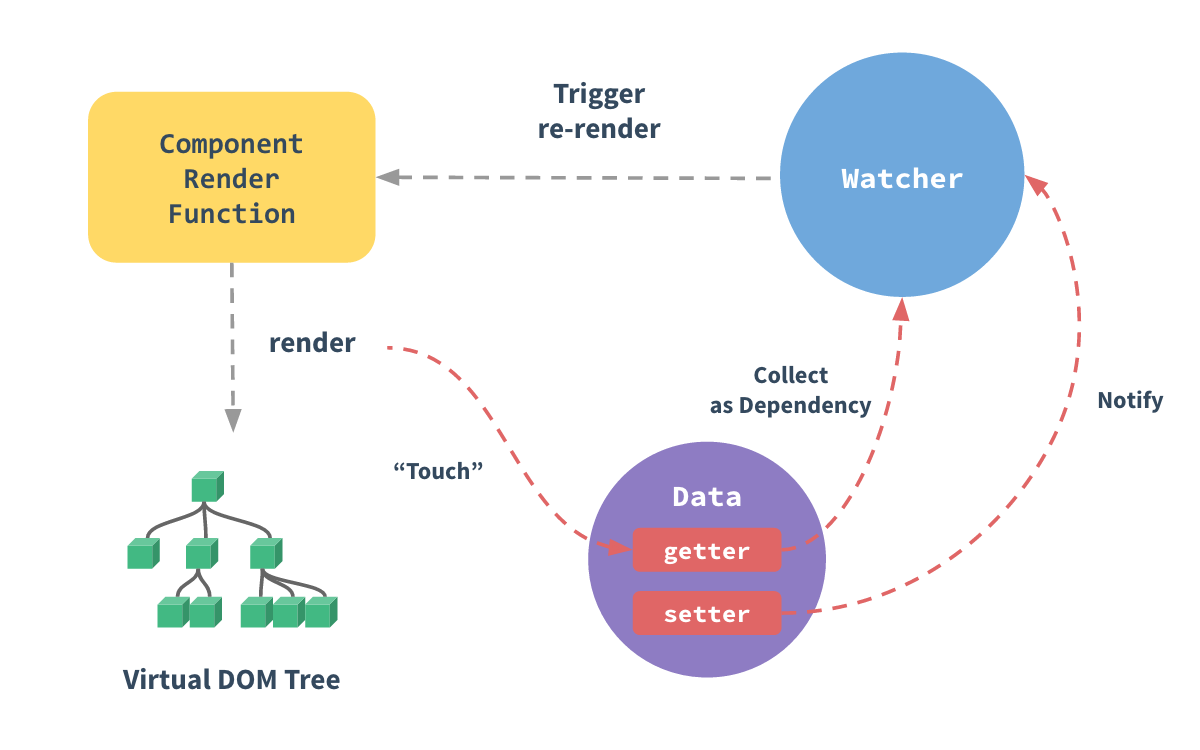
\includegraphics[scale=0.4]{data.png}
\caption{Vue响应式系统}
\end{figure}


\section{Detect Change}

受现代 Javascript 的限制(以及废弃 Object.observe),Vue 不能检测到对象属性的添加或删除。

由于 Vue 会在初始化实例时对属性执行 getter/setter 转化过程,所以属性必须在 data 对象上存在才能让 Vue 转换它,这样才能让它是响应式的。例如:



\begin{lstlisting}[language=JavaScript]
var vm = new Vue({
  data:{
  a:1
  }
})
// `vm.a` 是响应的
vm.b = 2
// `vm.b` 是非响应的
\end{lstlisting}

Vue 不允许在已经创建的实例上动态添加新的根级响应式属性(root-level reactive property),然而它可以使用 \texttt{Vue.set(object, key, value)} 方法将响应属性添加到嵌套的对象上:



\begin{lstlisting}[language=JavaScript]
Vue.set(vm.someObject, 'b', 2)
\end{lstlisting}

还可以使用 \texttt{vm.\$set}实例方法,这也是全局 Vue.set 方法的别名:



\begin{lstlisting}[language=JavaScript]
this.$set(this.someObject,'b',2)
\end{lstlisting}

有时需要向已有对象上添加一些属性,例如使用 Object.assign() 或 \_.extend() 方法来添加属性。但是,添加到对象上的新属性不会触发更新。在这种情况下可以创建一个新的对象,让它包含原对象的属性和新的属性:

\begin{lstlisting}[language=JavaScript]
// 代替 `Object.assign(this.someObject, { a: 1, b: 2 })`
this.someObject = Object.assign({}, this.someObject, { a: 1, b: 2 })
\end{lstlisting}


在列表渲染中也有一些数组相关的问题。




\begin{lstlisting}[language=JavaScript]

\end{lstlisting}



\begin{lstlisting}[language=JavaScript]

\end{lstlisting}






\begin{lstlisting}[language=JavaScript]

\end{lstlisting}



\begin{lstlisting}[language=JavaScript]

\end{lstlisting}






\begin{lstlisting}[language=JavaScript]

\end{lstlisting}



\begin{lstlisting}[language=JavaScript]

\end{lstlisting}




\part{Vue VM}


\chapter{Overview}





\chapter{VM Property}


\section{vm.\$el}








\begin{lstlisting}[language=JavaScript]

\end{lstlisting}




\begin{lstlisting}[language=JavaScript]

\end{lstlisting}




\begin{lstlisting}[language=JavaScript]

\end{lstlisting}






\section{vm.\$data}






\begin{lstlisting}[language=JavaScript]

\end{lstlisting}




\begin{lstlisting}[language=JavaScript]

\end{lstlisting}




\begin{lstlisting}[language=JavaScript]

\end{lstlisting}

\section{vm.\$options}








\begin{lstlisting}[language=JavaScript]

\end{lstlisting}




\begin{lstlisting}[language=JavaScript]

\end{lstlisting}




\begin{lstlisting}[language=JavaScript]

\end{lstlisting}




\section{vm.\$parent}







\begin{lstlisting}[language=JavaScript]

\end{lstlisting}




\begin{lstlisting}[language=JavaScript]

\end{lstlisting}




\begin{lstlisting}[language=JavaScript]

\end{lstlisting}



\section{vm.\$root}








\begin{lstlisting}[language=JavaScript]

\end{lstlisting}




\begin{lstlisting}[language=JavaScript]

\end{lstlisting}




\begin{lstlisting}[language=JavaScript]

\end{lstlisting}



\section{vm.\$children}








\begin{lstlisting}[language=JavaScript]

\end{lstlisting}




\begin{lstlisting}[language=JavaScript]

\end{lstlisting}




\begin{lstlisting}[language=JavaScript]

\end{lstlisting}



\section{vm.\$slots}










\begin{lstlisting}[language=JavaScript]

\end{lstlisting}




\begin{lstlisting}[language=JavaScript]

\end{lstlisting}




\begin{lstlisting}[language=JavaScript]

\end{lstlisting}


\section{vm.\$scopedSlots}








\begin{lstlisting}[language=JavaScript]

\end{lstlisting}




\begin{lstlisting}[language=JavaScript]

\end{lstlisting}




\begin{lstlisting}[language=JavaScript]

\end{lstlisting}



\section{vm.\$refs}








\begin{lstlisting}[language=JavaScript]

\end{lstlisting}




\begin{lstlisting}[language=JavaScript]

\end{lstlisting}




\begin{lstlisting}[language=JavaScript]

\end{lstlisting}




\section{vm.\$isServer}








\begin{lstlisting}[language=JavaScript]

\end{lstlisting}




\begin{lstlisting}[language=JavaScript]

\end{lstlisting}




\begin{lstlisting}[language=JavaScript]

\end{lstlisting}




\chapter{VM Method}


\section{VM Method Data}


\subsection{vm.\$watch}









\begin{lstlisting}[language=JavaScript]

\end{lstlisting}




\begin{lstlisting}[language=JavaScript]

\end{lstlisting}




\begin{lstlisting}[language=JavaScript]

\end{lstlisting}


\subsection{vm.\$set}








\begin{lstlisting}[language=JavaScript]

\end{lstlisting}




\begin{lstlisting}[language=JavaScript]

\end{lstlisting}




\begin{lstlisting}[language=JavaScript]

\end{lstlisting}




\subsection{vm.\$delete}








\begin{lstlisting}[language=JavaScript]

\end{lstlisting}




\begin{lstlisting}[language=JavaScript]

\end{lstlisting}




\begin{lstlisting}[language=JavaScript]

\end{lstlisting}











\begin{lstlisting}[language=JavaScript]

\end{lstlisting}




\begin{lstlisting}[language=JavaScript]

\end{lstlisting}




\begin{lstlisting}[language=JavaScript]

\end{lstlisting}




\section{VM Method Event}


\subsection{vm.\$on}








\begin{lstlisting}[language=JavaScript]

\end{lstlisting}




\begin{lstlisting}[language=JavaScript]

\end{lstlisting}




\begin{lstlisting}[language=JavaScript]

\end{lstlisting}



\subsection{vm.\$once}








\begin{lstlisting}[language=JavaScript]

\end{lstlisting}




\begin{lstlisting}[language=JavaScript]

\end{lstlisting}




\begin{lstlisting}[language=JavaScript]

\end{lstlisting}




\subsection{vm.\$off}








\begin{lstlisting}[language=JavaScript]

\end{lstlisting}




\begin{lstlisting}[language=JavaScript]

\end{lstlisting}




\begin{lstlisting}[language=JavaScript]

\end{lstlisting}




\subsection{vm.\$emit}








\begin{lstlisting}[language=JavaScript]

\end{lstlisting}




\begin{lstlisting}[language=JavaScript]

\end{lstlisting}




\begin{lstlisting}[language=JavaScript]

\end{lstlisting}




\section{VM Method Lifecycle}


\subsection{vm.\$mount}










\begin{lstlisting}[language=JavaScript]

\end{lstlisting}




\begin{lstlisting}[language=JavaScript]

\end{lstlisting}




\begin{lstlisting}[language=JavaScript]

\end{lstlisting}



\subsection{vm.\$forceUpdate}








\begin{lstlisting}[language=JavaScript]

\end{lstlisting}




\begin{lstlisting}[language=JavaScript]

\end{lstlisting}




\begin{lstlisting}[language=JavaScript]

\end{lstlisting}




\subsection{vm.\$nextTick}








\begin{lstlisting}[language=JavaScript]

\end{lstlisting}




\begin{lstlisting}[language=JavaScript]

\end{lstlisting}




\begin{lstlisting}[language=JavaScript]

\end{lstlisting}




\subsection{vm.\$destroy}








\begin{lstlisting}[language=JavaScript]

\end{lstlisting}




\begin{lstlisting}[language=JavaScript]

\end{lstlisting}




\begin{lstlisting}[language=JavaScript]

\end{lstlisting}














\begin{lstlisting}[language=JavaScript]

\end{lstlisting}




\begin{lstlisting}[language=JavaScript]

\end{lstlisting}




\begin{lstlisting}[language=JavaScript]

\end{lstlisting}















\begin{lstlisting}[language=JavaScript]

\end{lstlisting}




\begin{lstlisting}[language=JavaScript]

\end{lstlisting}




\begin{lstlisting}[language=JavaScript]

\end{lstlisting}




\begin{lstlisting}[language=JavaScript]

\end{lstlisting}




\begin{lstlisting}[language=JavaScript]

\end{lstlisting}




\begin{lstlisting}[language=JavaScript]

\end{lstlisting}






\part{Vue VNode}

\chapter{Overview}







\begin{lstlisting}[language=JavaScript]
/* @flow */

export default class VNode {
  tag: string | void;
  data: VNodeData | void;
  children: ?Array<VNode>;
  text: string | void;
  elm: Node | void;
  ns: string | void;
  context: Component | void; // rendered in this component's scope
  functionalContext: Component | void; // only for functional component root nodes
  key: string | number | void;
  componentOptions: VNodeComponentOptions | void;
  componentInstance: Component | void; // component instance
  parent: VNode | void; // component placeholder node
  raw: boolean; // contains raw HTML? (server only)
  isStatic: boolean; // hoisted static node
  isRootInsert: boolean; // necessary for enter transition check
  isComment: boolean; // empty comment placeholder?
  isCloned: boolean; // is a cloned node?
  isOnce: boolean; // is a v-once node?

  constructor (
    tag?: string,
    data?: VNodeData,
    children?: ?Array<VNode>,
    text?: string,
    elm?: Node,
    context?: Component,
    componentOptions?: VNodeComponentOptions
  ) {
    this.tag = tag
    this.data = data
    this.children = children
    this.text = text
    this.elm = elm
    this.ns = undefined
    this.context = context
    this.functionalContext = undefined
    this.key = data && data.key
    this.componentOptions = componentOptions
    this.componentInstance = undefined
    this.parent = undefined
    this.raw = false
    this.isStatic = false
    this.isRootInsert = true
    this.isComment = false
    this.isCloned = false
    this.isOnce = false
  }

  // DEPRECATED: alias for componentInstance for backwards compat.
  /* istanbul ignore next */
  get child (): Component | void {
    return this.componentInstance
  }
}

export const createEmptyVNode = () => {
  const node = new VNode()
  node.text = ''
  node.isComment = true
  return node
}

export function createTextVNode (val: string | number) {
  return new VNode(undefined, undefined, undefined, String(val))
}

// optimized shallow clone
// used for static nodes and slot nodes because they may be reused across
// multiple renders, cloning them avoids errors when DOM manipulations rely
// on their elm reference.
export function cloneVNode (vnode: VNode): VNode {
  const cloned = new VNode(
    vnode.tag,
    vnode.data,
    vnode.children,
    vnode.text,
    vnode.elm,
    vnode.context,
    vnode.componentOptions
  )
  cloned.ns = vnode.ns
  cloned.isStatic = vnode.isStatic
  cloned.key = vnode.key
  cloned.isCloned = true
  return cloned
}

export function cloneVNodes (vnodes: Array<VNode>): Array<VNode> {
  const res = new Array(vnodes.length)
  for (let i = 0; i < vnodes.length; i++) {
    res[i] = cloneVNode(vnodes[i])
  }
  return res
}
\end{lstlisting}




\begin{lstlisting}[language=JavaScript]

\end{lstlisting}




\begin{lstlisting}[language=JavaScript]

\end{lstlisting}




\begin{lstlisting}[language=JavaScript]

\end{lstlisting}




\begin{lstlisting}[language=JavaScript]

\end{lstlisting}




\begin{lstlisting}[language=JavaScript]

\end{lstlisting}



\part{Guideline}


\chapter{Overview}




\chapter{card}



\begin{lstlisting}[language=JavaScript]
<template>
  <section class="card" :class="{ 'little': is_little, 'no-padding': !use_padding }">
    <slot name="card-header"></slot>
    <slot name="card-neck"></slot>
    <slot></slot>
  </section>
</template>

<style scoped>
  .card { position: relative; padding-top: 18px; padding-bottom: 18px; }
  .card.little { padding-top: 0; padding-bottom: 0; margin-bottom: 12px; }
  /* 状态 */
  .card.no-padding { padding-top: 0; padding-bottom: 0; }
</style>

<script>
  export default {
    props: {
      is_little: { type: Boolean, default: false },
      use_padding: { type: Boolean, default: true }
    }
  };
</script>
\end{lstlisting}

\section{card\_header}



\begin{lstlisting}[language=JavaScript]
<template>
  <header class="card-header" :class="{ 'in-little-card': $parent.is_little }">
    <div class="card-header-main">{{ title }}
      <slot name="after-title"></slot>
    </div>
    <aside class="card-header-actions">
      <span v-show="is_save_actions_show">
        <btn :icon="'i-undo'" @click.native="$emit('reset-form')"></btn>
        <btn :icon="'i-check'" :text="'保存'" :mood="'emphasis'" @click.native="$emit('save-form')"></btn>
      </span>
      <slot></slot>
      <btn v-if="use_delete" :icon="'i-bin'" :mood="'danger'" @click.native="doDelete"></btn>
    </aside>
  </header>
</template>

<style scoped lang="stylus">
  @import "~styles/variables.styl";
  .card-header { position: relative; line-height: row_height_1; border-bottom: 1px solid light_gray_1; margin-bottom: 10px; }
  .card-header-main { font-weight: bold; }
  .card-header-main .icon { width: 12px; height: 12px; vertical-align: -2px; margin-left: 5px; }
  .card-header-actions { position: absolute; bottom: 2px; right: 2px; }
  /* 类型 */
  .card-header.in-little-card { background: #fff; padding: 2px 10px; height: 26px; margin-bottom: 0; border: none; }
</style>

<script>
  export default {
    props: {
      title: String,
      use_delete: { type: Boolean, default: false },
      is_save_actions_show: { type: Boolean, default: false },
      in_little_card: { type: Boolean, default: false }
    },
    methods: {
      doDelete: function (row, index) {
        if (window.confirm('确认删除?')) {
          this.$emit('do-delete', row, index);
        }
      }
    }
  };
</script>

\end{lstlisting}


\section{card\_neck}


\begin{lstlisting}[language=JavaScript]
<template>
  <aside class="card-neck">
    <slot></slot>
  </aside>
</template>

<style scoped>
  .card-neck { margin-bottom: 10px; }
  .card-neck > *:not(:first-child) { margin-left: 1px; }
</style>
\end{lstlisting}


\section{card\_footer}


\begin{lstlisting}[language=JavaScript]
<template>
  <header class="card-footer" :style="{ 'text-align': align }">
    <slot></slot>
  </header>
</template>

<style scoped lang="stylus">
  @import './../../../_styles/variables';
  .card-footer { position: relative; line-height: row_height_1; padding: 2px 0 5px; border-top: 1px solid light_gray_1; margin-top: 10px; }
</style>

<script>
  export default {
    props: {
      align: { type: String, default: 'right' }
    }
  };
</script>
\end{lstlisting}



\begin{lstlisting}[language=JavaScript]

\end{lstlisting}



\begin{lstlisting}[language=JavaScript]

\end{lstlisting}




\begin{lstlisting}[language=JavaScript]

\end{lstlisting}



\begin{lstlisting}[language=JavaScript]

\end{lstlisting}



\begin{lstlisting}[language=JavaScript]

\end{lstlisting}




\begin{lstlisting}[language=JavaScript]

\end{lstlisting}



\begin{lstlisting}[language=JavaScript]

\end{lstlisting}



\begin{lstlisting}[language=JavaScript]

\end{lstlisting}



\begin{lstlisting}[language=JavaScript]

\end{lstlisting}




\begin{lstlisting}[language=JavaScript]

\end{lstlisting}



\begin{lstlisting}[language=JavaScript]

\end{lstlisting}



\begin{lstlisting}[language=JavaScript]

\end{lstlisting}




\begin{lstlisting}[language=JavaScript]

\end{lstlisting}




\begin{lstlisting}[language=JavaScript]

\end{lstlisting}



\begin{lstlisting}[language=JavaScript]

\end{lstlisting}



\begin{lstlisting}[language=JavaScript]

\end{lstlisting}




\begin{lstlisting}[language=JavaScript]

\end{lstlisting}



\begin{lstlisting}[language=JavaScript]

\end{lstlisting}



\begin{lstlisting}[language=JavaScript]

\end{lstlisting}




\begin{lstlisting}[language=JavaScript]

\end{lstlisting}





\begin{lstlisting}[language=JavaScript]

\end{lstlisting}



\begin{lstlisting}[language=JavaScript]

\end{lstlisting}



\begin{lstlisting}[language=JavaScript]

\end{lstlisting}




\begin{lstlisting}[language=JavaScript]

\end{lstlisting}



\begin{lstlisting}[language=JavaScript]

\end{lstlisting}



\begin{lstlisting}[language=JavaScript]

\end{lstlisting}




\begin{lstlisting}[language=JavaScript]

\end{lstlisting}




\begin{lstlisting}[language=JavaScript]

\end{lstlisting}



\begin{lstlisting}[language=JavaScript]

\end{lstlisting}



\begin{lstlisting}[language=JavaScript]

\end{lstlisting}




\begin{lstlisting}[language=JavaScript]

\end{lstlisting}



\begin{lstlisting}[language=JavaScript]

\end{lstlisting}



\begin{lstlisting}[language=JavaScript]

\end{lstlisting}




\begin{lstlisting}[language=JavaScript]

\end{lstlisting}


\chapter{table\_grid}

\begin{lstlisting}[language=JavaScript]
<template>
  <section class="table-grid" :class="{ 'is-sortable': use_sort }">

    <!-- table header -->
    <header class="table-header" v-if="data_source.length > 0">
      <span class="table-header-col" v-if="use_sort" style="width: 35px;"><span>排序</span></span>
      <span class="table-header-col" v-for="col in cols"
            :style="[getWidth(col.span), { 'text-align': col.align }]"><span v-html="col.col_title"></span></span>
    </header>

    <transition :name="page_transition" :mode="'out-in'">
      <div class="table-body" v-if="data_source.length > 0" :key="transition_key">
        <draggable :list="data_source" :options="{ disabled: !use_sort, animation: 150, handle: '.drag-handle' }"
                   @end="doSort">
          <slot></slot>
        </draggable>
      </div>
    </transition>

    <aside class="text-center" v-if="!data_source.length > 0">~ Empty ~</aside>

  </section>
</template>

<style scoped lang="stylus">
  @import '~styles/variables.styl';
  .table-grid { position: relative; height: 100%; }
  .table-header { position: absolute; top: 0; left: 0; right: 0; z-index: 100; display: flex; line-height: row_height_2_inner; white-space: nowrap; box-shadow: 0 1px 2px -1px rgba(0, 0, 0, .3); }
  .table-header-col { background: #fff; padding: 0 8px; font-weight: bold; }
  .table-header-col > span { display: block; transform: scale(.9); transform-origin: 0 100%; }
  .table-body { height: 100%; padding-top: row_height_2_inner; overflow-y: auto; }
  /* 类型 */
  .row-action.blue { color: blue; }
  .row-action.warning { color: warning; }
  .row-action.danger { color: danger; }
  .row-action.success { color: success; }
</style>

<script>
  import color from 'styles/color.js';
  export default {
    props: {
      data_source: [Array, Object],
      active_index: Number,
      use_delete: { type: Boolean, default: false },
      use_sort: { type: Boolean, default: false },
      page_num: Number,
      transition_key: String
    },
    data () {
      return {
        color: color,
        rows: [],
        cols: [],
        page_transition: 'slide-right'
      };
    },
    watch: {
      data_source: function () {
        this.$nextTick(() => {
          this.initTable();
        });
      },
      page_num: function (new_page_num, old_page_num) {
        this.page_transition = new_page_num >= old_page_num ? 'slide-right' : 'slide-left';
      }
    },
    mounted: function () {
      this.$nextTick(() => {
        if (this.data_source.length > 0) {
          this.initTable();
        }
      });
    },
    methods: {
      initTable: function () {
        var rows = [];
        var closest_children = this.$children[0];
        if (!closest_children || !closest_children.$slots.default) return;
        closest_children.$slots.default.map((VNode) => {
          if (VNode.child) rows.push(VNode.child);
        });
        var cols = [];
        rows[0].$slots.default.map((VNode) => {
          if (VNode.child) cols.push(VNode.child);
        });
        this.rows = rows;
        this.cols = cols;
      },
      doSort: function (event) {
        this.$emit('do-sort', this.data_source[event.newIndex || 0], event.newIndex || 0, event.oldIndex);
      },
      getWidth: function (span) {
        if (!span) return { 'flex': 1 };
        else if (typeof span === 'string') return { 'width': span };
        else return { 'flex': span };
      }
    }
  };
</script>
\end{lstlisting}


\section{template}



\section{style}



\section{script}


\chapter{table\_grid\_2}


\begin{lstlisting}[language=JavaScript]
<template>
  <section class="table-grid" :class="{ 'is-sortable': use_sort }">

    <!-- table header -->
    <header class="table-header" v-if="data_source.length > 0">
      <span class="table-header-col" v-if="use_sort" style="width: 35px;"><span>排序</span></span>
      <span class="table-header-col" v-for="col in cols"
            :style="[getWidth(col.span), { 'text-align': col.align }]"><span v-html="col.col_title"></span></span>
    </header>

    <transition :name="page_transition" :mode="'out-in'">
      <div class="table-body" v-if="data_source.length > 0" :key="transition_key">
        <draggable :list="data_source" :options="{ disabled: !use_sort, animation: 150, handle: '.drag-handle' }"
                   @end="doSort">
          <slot></slot>
        </draggable>
      </div>
    </transition>

    <aside class="text-center" v-if="!data_source.length > 0">~ Empty ~</aside>

  </section>
</template>

<style scoped lang="stylus">
  @import '~styles/variables.styl';
  .table-grid { position: relative; height: 100%; }
  .table-header { position: absolute; top: 0; left: 0; right: 0; z-index: 100; display: flex; line-height: row_height_2_inner; white-space: nowrap; box-shadow: 0 1px 2px -1px rgba(0, 0, 0, .3); }
  .table-header-col { background: #fff; padding: 0 8px; font-weight: bold; }
  .table-header-col > span { display: block; transform: scale(.9); transform-origin: 0 100%; }
  .table-body { height: 100%; padding-top: row_height_2_inner; overflow-y: auto; }
  /* 类型 */
  .row-action.blue { color: blue; }
  .row-action.warning { color: warning; }
  .row-action.danger { color: danger; }
  .row-action.success { color: success; }
</style>

<script>
  import color from 'styles/color.js';
  export default {
    props: {
      data_source: [Array, Object],
      active_index: Number,
      use_delete: { type: Boolean, default: false },
      use_sort: { type: Boolean, default: false },
      page_num: Number,
      transition_key: String
    },
    data () {
      return {
        color: color,
        rows: [],
        cols: [],
        page_transition: 'slide-right'
      };
    },
    watch: {
      data_source: function () {
        this.$nextTick(() => {
          this.initTable();
        });
      },
      page_num: function (new_page_num, old_page_num) {
        this.page_transition = new_page_num >= old_page_num ? 'slide-right' : 'slide-left';
      }
    },
    mounted: function () {
      this.$nextTick(() => {
        if (this.data_source.length > 0) {
          this.initTable();
        }
      });
    },
    methods: {
      initTable: function () {
        var rows = [];
        var closest_children = this.$children[0];
        if (!closest_children || !closest_children.$slots.default) return;
        closest_children.$slots.default.map((VNode) => {
          if (VNode.child) rows.push(VNode.child);
        });
        var cols = [];
        rows[0].$slots.default.map((VNode) => {
          if (VNode.child) cols.push(VNode.child);
        });
        this.rows = rows;
        this.cols = cols;
      },
      doSort: function (event) {
        this.$emit('do-sort', this.data_source[event.newIndex || 0], event.newIndex || 0, event.oldIndex);
      },
      getWidth: function (span) {
        if (!span) return { 'flex': 1 };
        else if (typeof span === 'string') return { 'width': span };
        else return { 'flex': span };
      }
    }
  };
</script>
\end{lstlisting}



\begin{lstlisting}[language=JavaScript]

\end{lstlisting}




\begin{lstlisting}[language=JavaScript]

\end{lstlisting}

\chapter{table\_grid\_row}

\begin{lstlisting}[language=JavaScript]
<template>
  <section class="table-grid-row" :class="{ 'highlight': is_highlight, 'can-be-click': use_click }">
    <table-grid-col class="drag-handle" v-if="$parent.$parent.use_sort" :span="'35px'">
      <icon :name="'i-sort'" :color="'#666'"></icon>
    </table-grid-col>
    <slot></slot>
  </section>
</template>

<style scoped lang="stylus">
  @import '~styles/variables.styl';
  .table-grid-row { display: flex; margin-top: 1px; background: #fff; box-shadow: 0 1px 2px -1px rgba(0, 0, 0, .1); transition: all .2s; }
  .table-grid-row .icon { width: 12px; height: 12px; vertical-align: middle; }
  .table-grid-row .drag-handle { cursor: move; cursor: -webkit-grabbing; text-align: center; }
  .table-grid-row.highlight { background: light_gray_2; }
  .table-grid-row.can-be-click:not(.highlight):hover { background: light_gray_3; cursor: pointer; }
</style>

<script>
  export default {
    props: {
      dd: String,
      is_highlight: { type: Boolean, default: false },
      use_click: { type: Boolean, default: false }
    }
  };
</script>

\end{lstlisting}

\chapter{table\_grid\_col}

\begin{lstlisting}[language=JavaScript]
<template>
  <section class="table-grid-col"
           :title="!span || span > 0 ? $slots.default[0].text : ''"
           :style="[getWidth, { 'text-align': align }]">
    <slot></slot>
  </section>
</template>

<style scoped lang="stylus">
  @import '~styles/variables.styl';
  .table-grid-col { padding: 10px 8px; line-height: row_height_1; white-space: nowrap; overflow: hidden; text-overflow: ellipsis; }
  /* drag */
  .table-grid-row.sortable-ghost .table-grid-col { background: rgba(0, 0, 0, .02); }
</style>

<script>
  export default {
    props: {
      col_title: String,
      span: [String, Number],
      align: String
    },
    computed: {
      getWidth: function () {
        if (!this.span) return { 'flex': 1 };
        else if (typeof this.span === 'string') return { 'width': this.span };
        else return { 'flex': this.span };
      }
    }
  };
</script>

\end{lstlisting}




\begin{lstlisting}[language=JavaScript]

\end{lstlisting}



\begin{lstlisting}[language=JavaScript]

\end{lstlisting}



\begin{lstlisting}[language=JavaScript]

\end{lstlisting}



\begin{lstlisting}[language=JavaScript]

\end{lstlisting}




\begin{lstlisting}[language=JavaScript]

\end{lstlisting}



\begin{lstlisting}[language=JavaScript]

\end{lstlisting}



\begin{lstlisting}[language=JavaScript]

\end{lstlisting}




\begin{lstlisting}[language=JavaScript]

\end{lstlisting}




\begin{lstlisting}[language=JavaScript]

\end{lstlisting}



\begin{lstlisting}[language=JavaScript]

\end{lstlisting}



\begin{lstlisting}[language=JavaScript]

\end{lstlisting}




\begin{lstlisting}[language=JavaScript]

\end{lstlisting}



\begin{lstlisting}[language=JavaScript]

\end{lstlisting}



\begin{lstlisting}[language=JavaScript]

\end{lstlisting}




\begin{lstlisting}[language=JavaScript]

\end{lstlisting}





\begin{lstlisting}[language=JavaScript]

\end{lstlisting}



\begin{lstlisting}[language=JavaScript]

\end{lstlisting}



\begin{lstlisting}[language=JavaScript]

\end{lstlisting}




\begin{lstlisting}[language=JavaScript]

\end{lstlisting}



\begin{lstlisting}[language=JavaScript]

\end{lstlisting}



\begin{lstlisting}[language=JavaScript]

\end{lstlisting}




\begin{lstlisting}[language=JavaScript]

\end{lstlisting}




\begin{lstlisting}[language=JavaScript]

\end{lstlisting}



\begin{lstlisting}[language=JavaScript]

\end{lstlisting}



\begin{lstlisting}[language=JavaScript]

\end{lstlisting}




\begin{lstlisting}[language=JavaScript]

\end{lstlisting}



\begin{lstlisting}[language=JavaScript]

\end{lstlisting}



\begin{lstlisting}[language=JavaScript]

\end{lstlisting}




\begin{lstlisting}[language=JavaScript]

\end{lstlisting}



\part{Kitchen}

\chapter{Overview}



\chapter{Kitchen}

index.html的内容如下:


\begin{lstlisting}[language=HTML]
<!DOCTYPE html>
<html>
  <head>
    <meta charset="utf-8">
    <title>hi-kitchen</title>
  </head>
  <body>
    <div id="app"></div>
    <!-- built files will be auto injected -->
  </body>
</html>
\end{lstlisting}


\section{build}


\subsection{build.js}


\begin{lstlisting}[language=bash]
// https://github.com/shelljs/shelljs
require('shelljs/global')
env.NODE_ENV = 'production'

var path = require('path')
var config = require('../config')
var ora = require('ora')
var webpack = require('webpack')
var webpackConfig = require('./webpack.prod.conf')

console.log(
  '  Tip:\n' +
  '  Built files are meant to be served over an HTTP server.\n' +
  '  Opening index.html over file:// won\'t work.\n'
)

var spinner = ora('building for production...')
spinner.start()

var assetsPath = path.join(config.build.assetsRoot, config.build.assetsSubDirectory)
rm('-rf', assetsPath)
mkdir('-p', assetsPath)
cp('-R', 'static/*', assetsPath)

webpack(webpackConfig, function (err, stats) {
  spinner.stop()
  if (err) throw err
  process.stdout.write(stats.toString({
    colors: true,
    modules: false,
    children: false,
    chunks: false,
    chunkModules: false
  }) + '\n')
})
\end{lstlisting}

\subsection{dev-client.js}


\begin{lstlisting}[language=bash]
/* eslint-disable */
require('eventsource-polyfill')
var hotClient = require('webpack-hot-middleware/client?noInfo=true&reload=true')

hotClient.subscribe(function (event) {
  if (event.action === 'reload') {
    window.location.reload()
  }
})
\end{lstlisting}


\subsection{dev-server.js}


\begin{lstlisting}[language=bash]
var config = require('../config')
if (!process.env.NODE_ENV) process.env.NODE_ENV = config.dev.env
var path = require('path')
var express = require('express')
var webpack = require('webpack')
var opn = require('opn')
var proxyMiddleware = require('http-proxy-middleware')
var webpackConfig = require('./webpack.dev.conf')

// default port where dev server listens for incoming traffic
var port = process.env.PORT || config.dev.port
// Define HTTP proxies to your custom API backend
// https://github.com/chimurai/http-proxy-middleware
var proxyTable = config.dev.proxyTable

var app = express()
var compiler = webpack(webpackConfig)

var devMiddleware = require('webpack-dev-middleware')(compiler, {
  publicPath: webpackConfig.output.publicPath,
  stats: {
    colors: true,
    chunks: false
  }
})

var hotMiddleware = require('webpack-hot-middleware')(compiler)
// force page reload when html-webpack-plugin template changes
compiler.plugin('compilation', function (compilation) {
  compilation.plugin('html-webpack-plugin-after-emit', function (data, cb) {
    hotMiddleware.publish({ action: 'reload' })
    cb()
  })
})

// proxy api requests
Object.keys(proxyTable).forEach(function (context) {
  var options = proxyTable[context]
  if (typeof options === 'string') {
    options = { target: options }
  }
  app.use(proxyMiddleware(context, options))
})

// handle fallback for HTML5 history API
app.use(require('connect-history-api-fallback')())

// serve webpack bundle output
app.use(devMiddleware)

// enable hot-reload and state-preserving
// compilation error display
app.use(hotMiddleware)

// serve pure static assets
var staticPath = path.posix.join(config.dev.assetsPublicPath, config.dev.assetsSubDirectory)
app.use(staticPath, express.static('./static'))

module.exports = app.listen(port, function (err) {
  if (err) {
    console.log(err)
    return
  }
  var uri = 'http://localhost:' + port
  console.log('Listening at ' + uri + '\n')
  opn(uri)
})
\end{lstlisting}

\section{config}

\subsection{dev.env.js}


\begin{lstlisting}[language=bash]
var merge = require('webpack-merge')
var prodEnv = require('./prod.env')

module.exports = merge(prodEnv, {
  NODE_ENV: '"development"'
})
\end{lstlisting}


\subsection{prod.env.js}



\begin{lstlisting}[language=bash]
module.exports = {
  NODE_ENV: '"production"'
}
\end{lstlisting}

\subsection{index.js}

\begin{lstlisting}[language=bash]
// see http://vuejs-templates.github.io/webpack for documentation.
var path = require('path')

var common_proxy = {
  //target       : 'http://test.hitour.cc',
  //target       : 'http://sandbox.hitour.cc',
  target          : 'http://trial.hitour.cc',
  // target      : 'http://hitour.host',
  changeOrigin: true,
  pathRewrite: {}
};

module.exports = {
  build: {
    env: require('./prod.env'),
    index: path.resolve(__dirname, '../dist/index.html'),
    assetsRoot: path.resolve(__dirname, '../dist'),
    assetsSubDirectory: 'static',
    assetsPublicPath: '/themes/kitchen/dist/',
    productionSourceMap: true,
    // Gzip off by default as many popular static hosts such as
    // Surge or Netlify already gzip all static assets for you.
    // Before setting to `true`, make sure to:
    // npm install --save-dev compression-webpack-plugin
    productionGzip: false,
    productionGzipExtensions: ['js', 'css']
  },
  dev: {
    env: require('./dev.env'),
    port: 60003,
    assetsSubDirectory: 'static',
    assetsPublicPath: '/',
    proxyTable: {
      '/admin/': common_proxy,
      '/chef/': common_proxy,
      '/themes': common_proxy,
      '/markMi/': common_proxy
    },
    // CSS Sourcemaps off by default because relative paths are "buggy"
    // with this option, according to the CSS-Loader README
    // (https://github.com/webpack/css-loader#sourcemaps)
    // In our experience, they generally work as expected,
    // just be aware of this issue when enabling this option.
    cssSourceMap: false
  }
}
\end{lstlisting}

\section{views}


\subsection{\_components}


\begin{lstlisting}[language=bash]

\end{lstlisting}



\begin{lstlisting}[language=bash]

\end{lstlisting}


\subsection{\_router}



\begin{lstlisting}[language=bash]

\end{lstlisting}



\begin{lstlisting}[language=bash]

\end{lstlisting}



\subsection{\_store}


\begin{lstlisting}[language=bash]

\end{lstlisting}



\begin{lstlisting}[language=bash]

\end{lstlisting}



\subsection{\_styles}



\begin{lstlisting}[language=bash]

\end{lstlisting}



\begin{lstlisting}[language=bash]

\end{lstlisting}


\subsection{\_utils}




\begin{lstlisting}[language=bash]

\end{lstlisting}



\begin{lstlisting}[language=bash]

\end{lstlisting}



\chapter{\_components}


\begin{lstlisting}[language=bash]

\end{lstlisting}



\begin{lstlisting}[language=bash]

\end{lstlisting}



\chapter{\_router}


\section{index.js}



\begin{lstlisting}[language=bash]

\end{lstlisting}



\begin{lstlisting}[language=bash]

\end{lstlisting}



\section{library.js}



\begin{lstlisting}[language=bash]

\end{lstlisting}



\begin{lstlisting}[language=bash]

\end{lstlisting}


\section{operation.js}




\begin{lstlisting}[language=bash]
export default {
  path: 'operation',
  name: 'operation',
  component: require('views/desktop/operation/operation'),
  redirect: { name: 'operation_destination_nav' },
  children: [
    // ----------------------------------------------------------------------------------------
    // 目的地导航
    {
      path: 'destination_nav/:continent_id?/:continent_code?/:country_id?/:country_code?',
      name: 'operation_destination_nav',
      component: require('views/desktop/operation/destination_nav/destination_nav')
    },
    // ----------------------------------------------------------------------------------------
    // 周边游导航
    {
      path: 'around_tour_nav/:first_level_id?/:first_level_code?/:second_level_id?/:second_level_code?',
      name: 'operation_around_tour_nav',
      component: require('views/desktop/operation/around_tour_nav/around_tour_nav')
    },
    // ----------------------------------------------------------------------------------------
    // 商品分组
    {
      path: 'product_group',
      name: 'operation_product_group',
      component: require('views/desktop/operation/product_group/product_group')
    },
    {
      path: 'product_group/:group_id/:tab',
      name: 'operation_product_group_detail',
      component: require('views/desktop/operation/product_group/product_group_detail')
    },
    // ----------------------------------------------------------------------------------------
    // 商品分组的分组
    {
      path: 'group_product_group',
      name: 'operation_group_product_group',
      component: require('views/desktop/operation/group_product_group/group_product_group')
    },
    {
      path: 'group_product_group/:group_id',
      name: 'operation_group_product_group_detail',
      component: require('views/desktop/operation/group_product_group/group_product_group_detail')
    },
    {
      path: 'group_product_group_in_group/:group_id/:tab',
      name: 'operation_product_group_detail_in_group',
      component: require('views/desktop/operation/group_product_group/product_group_detail_in_group')
    },
    // ----------------------------------------------------------------------------------------
    // 商户分组
    {
      path: 'merchant_group',
      name: 'operation_merchant_group',
      component: require('views/desktop/operation/merchant_group/merchant_group')
    },
    {
      path: 'merchant_group/:group_id/:tab',
      name: 'operation_merchant_group_detail',
      component: require('views/desktop/operation/merchant_group/merchant_group_detail')
    },
    // ----------------------------------------------------------------------------------------
    // Banner
    {
      path: 'banner',
      name: 'operation_banner',
      component: require('views/desktop/operation/banner/banner')
    },
    {
      path: 'banner/:banner_id',
      name: 'operation_banner_detail',
      component: require('views/desktop/operation/banner/banner_detail')
    },
    // ----------------------------------------------------------------------------------------
    // Tag
    {
      path: 'tag',
      name: 'operation_tag',
      component: require('views/desktop/operation/tag/tag')
    },
    {
      path: 'tag/:tag_id',
      name: 'operation_tag_detail',
      component: require('views/desktop/operation/tag/tag_detail')
    },
    // ----------------------------------------------------------------------------------------
    // web首页
    {
      path: 'web_home',
      name: 'operation_web_home',
      component: require('views/desktop/operation/web_home/web_home')
    },
    {
      path: 'web_home/:area_id/:tab',
      name: 'operation_web_home_area',
      component: require('views/desktop/operation/web_home/web_home_area')
    },
    {
      path: 'web_home_product_group/:group_id/:tab',
      name: 'operation_web_home_product_group_detail',
      component: require('views/desktop/operation/web_home/product_group_detail')
    },
    {
      path: 'web_home_group_product_group/:group_id',
      name: 'operation_web_home_group_product_group_detail',
      component: require('views/desktop/operation/web_home/group_product_group_detail')
    },
    {
      path: 'web_home/:area_id/:tab/banner/:banner_id',
      name: 'operation_web_home_banner_detail',
      component: require('views/desktop/operation/banner/banner_detail')
    },
    // ----------------------------------------------------------------------------------------
    // web目的地页
    {
      path: 'web_dest',
      name: 'operation_web_dest',
      component: require('views/desktop/operation/web_dest/web_dest')
    },
    {
      path: 'web_dest_detail/:dest_id/:dest_title/:dest_type/:tab/:country_code',
      name: 'operation_web_dest_detail',
      component: require('views/desktop/operation/web_dest/web_dest_detail')
    },
    // ----------------------------------------------------------------------------------------
    // 菠萝PASS
    {
      path: 'wxapp_bolo_city',
      name: 'operation_wxapp_bolo_city',
      component: require('views/desktop/operation/wxapp_bolo_city/wxapp_bolo_city')
    },
    {
      path: 'wxapp_bolo_city_detail/:city_code/:cn_name/:tab',
      name: 'operation_wxapp_bolo_city_detail',
      component: require('views/desktop/operation/wxapp_bolo_city/wxapp_bolo_city_detail')
    },
    {
      path: 'wxapp_bolo_gift_card',
      name: 'operation_wxapp_bolo_gift_card',
      component: require('views/desktop/operation/wxapp_bolo_gift_card/wxapp_bolo_gift_card')
    },
    {
      path: 'wxapp_bolo_gift_card_detail/:card_id/:tab',
      name: 'operation_wxapp_bolo_gift_card_detail',
      component: require('views/desktop/operation/wxapp_bolo_gift_card/wxapp_bolo_gift_card_detail')
    }
  ]
};
\end{lstlisting}



\begin{lstlisting}[language=bash]

\end{lstlisting}

\subsection{/k/desktop/operation/destination\_nav}


/k/desktop/operation默认跳转到/k/desktop/operaton/destination\_nav。



\section{order.js}


\begin{lstlisting}[language=bash]

\end{lstlisting}



\begin{lstlisting}[language=bash]

\end{lstlisting}


\section{resource.js}



\begin{lstlisting}[language=bash]
export default {
  path: 'resource',
  name: 'resource',
  component: require('views/desktop/resource/resource'),
  redirect: {name: 'resource_hotel'},
  children: [
    {
      path: 'hotel',
      name: 'resource_hotel',
      component: require('views/desktop/resource/ui_hotel/ui_hotel_list')
    },
    {
      path: 'hotel/:hotel_id/:tab',
      name: 'resource_hotel_detail',
      component: require('views/desktop/resource/ui_hotel/ui_hotel_detail')
    },
    {
      path: 'facility',
      name: 'resource_hotel_facility',
      component: require('views/desktop/resource/ui_hotel/ui_hotel_facility_list')
    },
    {
      path: 'facility/:facility_id',
      name: 'resource_hotel_facility_detail',
      component: require('views/desktop/resource/ui_hotel/ui_hotel_facility_detail')
    },
    {
      path: 'service',
      name: 'resource_hotel_service',
      component: require('views/desktop/resource/ui_hotel/ui_hotel_service_list')
    },
    {
      path: 'service/:service_id',
      name: 'resource_hotel_service_detail',
      component: require('views/desktop/resource/ui_hotel/ui_hotel_service_detail')
    },
    {
      path: 'hotel_room/:room_id/:hotel_id/:tab',
      name: 'resource_hotel_room_detail',
      component: require('views/desktop/resource/ui_hotel/ui_hotel_room_detail')
    },
    {
      path: 'rate',
      name: 'resource_rate',
      component: require('views/desktop/resource/ui_hotel/ui_rate_list')
    },
    {
      path: 'rate/:rate_id',
      name: 'resource_rate_detail',
      component: require('views/desktop/resource/ui_hotel/ui_rate_detail')
    },
    {
      path: 'traffic/:traffic_id/:hotel_id',
      name: 'resource_hotel_traffic_detail',
      component: require('views/desktop/resource/ui_hotel/ui_hotel_traffic_detail')
    },
    {
      path: 'tag',
      name: 'resource_hotel_tag',
      component: require('views/desktop/resource/ui_hotel/ui_hotel_tag_list')
    },
    {
      path: 'tag/:tag_id',
      name: 'resource_hotel_tag_detail',
      component: require('views/desktop/resource/ui_hotel/ui_hotel_tag_detail')
    },
    {
      path: 'hotel_rate/:hotel_id/:rate_source_id/:rate_id',
      name: 'resource_hotel_rate_detail',
      component: require('views/desktop/resource/ui_hotel/ui_hotel_rate_detail')
    },
    {
      path: 'flight',
      redirect: {name: 'resource_airline'}
    },
    {
      path: 'flight/airline',
      name: 'resource_airline',
      component: require('views/desktop/resource/ui_flight/ui_airline_list')
    },
    {
      path: 'flight/airline/:airline_id',
      name: 'resource_airline_detail',
      component: require('views/desktop/resource/ui_flight/ui_airline_detail')
    },
    {
      path: 'flight/airline/:tab',
      name: 'airline_detail',
      component: require('views/desktop/resource/ui_flight/ui_airline_detail')
    },
    {
      path: 'flight/airport',
      name: 'resource_airport',
      component: require('views/desktop/resource/ui_flight/ui_airport_list')
    },
    {
      path: 'flight/airport/:airport_id',
      name: 'resource_airport_detail',
      component: require('views/desktop/resource/ui_flight/ui_airport_detail')
    },
    {
      path: 'flight/airport/:tab',
      name: 'airport_detail',
      component: require('views/desktop/resource/ui_flight/ui_airport_detail')
    },
    {
      path: 'flight/aircraft',
      name: 'resource_aircraft',
      component: require('views/desktop/resource/ui_flight/ui_aircraft_list')
    },
    {
      path: 'flight/aircraft/:aircraft_id',
      name: 'resource_aircraft_detail',
      component: require('views/desktop/resource/ui_flight/ui_aircraft_detail')
    },
    {
      path: 'flight/aircraft/:tab',
      name: 'aircraft_detail',
      component: require('views/desktop/resource/ui_flight/ui_aircraft_detail')
    },
    {
      path: 'flight/list',
      name: 'resource_flight',
      component: require('views/desktop/resource/ui_flight/ui_flight_list')
    },
    {
      path: 'flight/:flight_no',
      name: 'resource_flight_detail',
      component: require('views/desktop/resource/ui_flight/ui_flight_detail')
    },
    {
      path: 'flight/:tab',
      name: 'new_resource_flight',
      component: require('views/desktop/resource/ui_flight/ui_flight_detail')
    }
  ]
};
\end{lstlisting}



\subsection{/k/desktop/resource/hotel}


\begin{lstlisting}[language=bash]

\end{lstlisting}


\section{sale\_rule.js}




\begin{lstlisting}[language=bash]

\end{lstlisting}



\begin{lstlisting}[language=bash]

\end{lstlisting}



\chapter{Resource}

\section{resource.js}

在\_router中设置resource的路由配置:


\begin{lstlisting}[language=bash]
export default {
   path: 'resource',
   name: 'resource',
   component: require('views/desktop/resource/resource'),
   redirect: { name: 'resource_hotel' },
   children: [
      {
        path: 'hotel',
        name: 'resource_hotel',
        component: require('views/desktop/resource/ui_hotel/ui_hotel_list')
      },
      {
        path: 'airline',
        name: 'resource_airline',
        component: require('views/desktop/resource/ui_airline/ui_airline_list')
      }
   ]
}
\end{lstlisting}



\begin{lstlisting}[language=bash]

\end{lstlisting}


\section{resource.vue}

\begin{lstlisting}[language=bash]
<template>
    <board :nav_groups="nav_groups"></board>
</template>

<script>
  export default {
    data () {
      return {
        nav_groups: [
          {
            group_name: '酒店基本信息',
            group_items: [
              { name: '酒店列表', route: { name: 'resource_hotel' } },
              { name: '酒店设施', route: { name: 'resource_hotel_facility' } },
              { name: '酒店服务', route: { name: 'resource_hotel_service' } },
              { name: '评分来源', route: { name: 'resource_rate' } },
              { name: '资源标签', route: { name: 'resource_hotel_tag' } }
            ]
          },
          {
            group_name: '机票基本信息',
            group_items: [
              { name: '航空公司', route: { name: 'resource_airline' } },
              { name: '机场信息', route: { name: 'resource_airport' } },
              { name: '机型列表', route: { name: 'resource_aircraft' } },
              { name: '航班信息', route: { name: 'resource_flight' } }
            ]
          }
        ]
      };
    }
  };
</script>
\end{lstlisting}




\subsection{board.vue}





\begin{lstlisting}[language=bash]
<template>
  <section class="board">
    <left-nav :nav_groups="nav_groups"></left-nav>
    <router-view class="" :class="{ 'move-left' : $store.state.is_cheat_sheet_show }"></router-view>
  </section>
</template>

<style scoped>
  .board .left-nav { position: fixed; top: 80px; width: 200px; }
  .board .paper-view { margin-left: 220px; }
  /*.board .paper-view.move-left { transform: translateX(-220px); }*/
  .board .paper-view.move-left { margin-left: 0; }
</style>

<script>
export default {
   props: ['nav_groups'],
   components: {
       'left-nav': require(`views/_components/left_nav')
   }
};
</script>
\end{lstlisting}






\begin{lstlisting}[language=bash]

\end{lstlisting}



\begin{lstlisting}[language=bash]

\end{lstlisting}






\begin{lstlisting}[language=bash]

\end{lstlisting}



\begin{lstlisting}[language=bash]

\end{lstlisting}






\begin{lstlisting}[language=bash]

\end{lstlisting}



\begin{lstlisting}[language=bash]

\end{lstlisting}






\begin{lstlisting}[language=bash]

\end{lstlisting}



\begin{lstlisting}[language=bash]

\end{lstlisting}






\begin{lstlisting}[language=bash]

\end{lstlisting}



\begin{lstlisting}[language=bash]

\end{lstlisting}





\begin{lstlisting}[language=bash]

\end{lstlisting}



\begin{lstlisting}[language=bash]

\end{lstlisting}






\begin{lstlisting}[language=bash]

\end{lstlisting}



\begin{lstlisting}[language=bash]

\end{lstlisting}






\begin{lstlisting}[language=bash]

\end{lstlisting}



\begin{lstlisting}[language=bash]

\end{lstlisting}






\begin{lstlisting}[language=bash]

\end{lstlisting}



\begin{lstlisting}[language=bash]

\end{lstlisting}






\begin{lstlisting}[language=bash]

\end{lstlisting}



\begin{lstlisting}[language=bash]

\end{lstlisting}






\begin{lstlisting}[language=bash]

\end{lstlisting}



\begin{lstlisting}[language=bash]

\end{lstlisting}






\begin{lstlisting}[language=bash]

\end{lstlisting}



\begin{lstlisting}[language=bash]

\end{lstlisting}






\begin{lstlisting}[language=bash]

\end{lstlisting}



\begin{lstlisting}[language=bash]

\end{lstlisting}





\begin{lstlisting}[language=bash]

\end{lstlisting}



\begin{lstlisting}[language=bash]

\end{lstlisting}






\begin{lstlisting}[language=bash]

\end{lstlisting}



\begin{lstlisting}[language=bash]

\end{lstlisting}






\begin{lstlisting}[language=bash]

\end{lstlisting}



\begin{lstlisting}[language=bash]

\end{lstlisting}






\begin{lstlisting}[language=bash]

\end{lstlisting}



\begin{lstlisting}[language=bash]

\end{lstlisting}






\begin{lstlisting}[language=bash]

\end{lstlisting}



\begin{lstlisting}[language=bash]

\end{lstlisting}






\begin{lstlisting}[language=bash]

\end{lstlisting}



\begin{lstlisting}[language=bash]

\end{lstlisting}






\begin{lstlisting}[language=bash]

\end{lstlisting}



\begin{lstlisting}[language=bash]

\end{lstlisting}






\begin{lstlisting}[language=bash]

\end{lstlisting}



\begin{lstlisting}[language=bash]

\end{lstlisting}





\begin{lstlisting}[language=bash]

\end{lstlisting}



\begin{lstlisting}[language=bash]

\end{lstlisting}






\begin{lstlisting}[language=bash]

\end{lstlisting}



\begin{lstlisting}[language=bash]

\end{lstlisting}






\begin{lstlisting}[language=bash]

\end{lstlisting}



\begin{lstlisting}[language=bash]

\end{lstlisting}






\begin{lstlisting}[language=bash]

\end{lstlisting}



\begin{lstlisting}[language=bash]

\end{lstlisting}






\begin{lstlisting}[language=bash]

\end{lstlisting}



\begin{lstlisting}[language=bash]

\end{lstlisting}






\begin{lstlisting}[language=bash]

\end{lstlisting}



\begin{lstlisting}[language=bash]

\end{lstlisting}






\begin{lstlisting}[language=bash]

\end{lstlisting}



\begin{lstlisting}[language=bash]

\end{lstlisting}







\chapter{分组接口}


\section{/chef/api/operation/productGroup/Group}


\subsection{GET}

获取分组详情

URL:\url{/chef/api/operation/productGroup/Group}





\begin{longtable}{|m{50pt}|m{40pt}|m{50pt}|m{50pt}|}
%head
\multicolumn{4}{r}{}
\tabularnewline\hline
字段&类型&必填&备注
\endhead
%endhead

%firsthead
\caption{获取分组详情接口-请求参数}\\
\hline
字段&类型&必填&备注
\endfirsthead
%endfirsthead

%foot
\multicolumn{4}{r}{}
\endfoot
%endfoot

%lastfoot
\endlastfoot
%endlastfoot
\hline
group\_id&int&是&分组ID\\
\hline
\end{longtable}

\begin{lstlisting}[language=JavaScript]
{
  "code": 200,
  "msg": "Ok.",
  "data": {
    "group_id": "19",
    "show_type": "0",
    "title": "扫货扫货qu去首尔",
    "sub_title": "特价机票+酒店",
    "short_desc": "",
    "route_desc": "首尔自由行特价机票酒店,1999起",
    "date_desc": "",
    "pc_image_url": "http://pics.hitour.cc/e969a4546e0228ebe7ed9ffe52319962.png",
    "h5_image_url": "",
    "icon_image_url": "",
    "start_date": "2016-08-23",
    "end_date": "2016-12-31",
    "status": "1",
    "type": "1",
    "group_dests": [
      {
        "id": "27",
        "group_id": "19",
        "dest_code": "1",
        "name": "华南",
        "type": "1",
        "display_order": "5"
      }
   ],
    "group_locations": [
      {
        "label_id": "1",
        "group_id": "19",
        "city_code": "SEL",
        "type": "3",
        "city": {
          "country_code": "KR",
          "city_code": "SEL",
          "iata_code": "SEL",
          "cn_name": "首尔",
          "en_name": "Seoul",
          "pinyin": "shou er",
          "timezone": "+9:00",
          "has_product": "1",
          "has_online_product": "1",
          "top_search": "[{\"value\":\"\\u4e50\\u5929\\u4e16\\u754c\",\"display_order\":1},{\"value\":\"\\u6c11\\u4fd7\",\"display_order\":2},{\"value\":\"\\u4e71\\u6253\\u79c0\",\"display_order\":3},{\"value\":\"\\u660e\\u6d1e\",\"display_order\":4},{\"value\":\"\\u6c5d\\u77e3\\u5c9b\",\"display_order\":5},{\"value\":\"\\u4e1c\\u5927\\u95e8\",\"display_order\":6}]",
          "data_level": "2",
          "show_in_country": "0",
          "link_url": "/South_Korea/Seoul",
          "link_url_m": "/mobile#/city/SEL",
          "city_name": "Seoul",
          "country_name": "South_Korea",
          "country_cn_name": "韩国"
        }
      }
    ],
    "group_products": [
         {
        "id": "44",
        "group_id": "19",
        "product_id": "8837",
        "display_order": "8",
        "product_description": {
          "name": "【秋游季】上海直飞首尔4-5天机酒自由行•五星航空韩亚往返机票+全程热销酒店套餐任选 赠接机半日游/首尔1日游/自由行大礼包",
          "product_id": "8837",
          "language_id": "2"
        }
      }
    ]
  }
}
\end{lstlisting}


\subsection{POST}

新增分组

URL:\url{/chef/api/operation/productGroup/Group}



\begin{longtable}{|m{80pt}|m{40pt}|m{50pt}|m{150pt}|}
%head
\multicolumn{4}{r}{}
\tabularnewline\hline
字段&类型&必填&备注
\endhead
%endhead

%firsthead
\caption{新增分组接口-请求参数}\\
\hline
字段&类型&必填&备注
\endfirsthead
%endfirsthead

%foot
\multicolumn{4}{r}{}
\endfoot
%endfoot

%lastfoot
\endlastfoot
%endlastfoot
\hline
title			&string	&是	&唯一\\
\hline
sub\_title	&string	&否	&副标题\\
\hline
short\_desc	&string	&否	&短标题\\
\hline
route\_desc	&string	&是	&专题线路\\
\hline
date\_desc	&string	&是	&专题日期\\
\hline
pc\_image\_url&string	&否	&\\
\hline
h5\_image\_url&string	&否	&\\
\hline
icon\_image\_url&string&否	&\\
\hline
start\_date	&date	&是	&\\
\hline
end\_date	&date	&是	&\\
\hline
type			&int		&是	&1普通分组,2是父级分组\\
\hline
city\_code	&array	&是	&城市\\
\hline
\end{longtable}


\begin{lstlisting}[language=JavaScript]
{
  "code": 200,
  "msg": "Ok.",
  "data": {
    "show_type": 0,
    "title": "扫货扫货401",
    "sub_title": "lalaa",
    "short_desc": "",
    "route_desc": "",
    "date_desc": "",
    "start_date": "0000-00-00",
    "end_date": "0000-00-00",
    "status": 0,
    "type": 1,
    "group_id": "49",
    "pc_image_url": null,
    "h5_image_url": null,
    "icon_image_url": null,
    "group_locations": [
      {
        "label_id": "1",
        "group_id": "19",
        "city_code": "SEL",
        "type": "3",
        "city": {
          "country_code": "KR",
          "city_code": "SEL",
          "iata_code": "SEL",
          "cn_name": "首尔",
          "en_name": "Seoul",
          "pinyin": "shou er",
          "timezone": "+9:00",
          "has_product": "1",
          "has_online_product": "1",
          "top_search": "[{\"value\":\"\\u4e50\\u5929\\u4e16\\u754c\",\"display_order\":1},{\"value\":\"\\u6c11\\u4fd7\",\"display_order\":2},{\"value\":\"\\u4e71\\u6253\\u79c0\",\"display_order\":3},{\"value\":\"\\u660e\\u6d1e\",\"display_order\":4},{\"value\":\"\\u6c5d\\u77e3\\u5c9b\",\"display_order\":5},{\"value\":\"\\u4e1c\\u5927\\u95e8\",\"display_order\":6}]",
          "data_level": "2",
          "show_in_country": "0",
          "link_url": "/South_Korea/Seoul",
          "link_url_m": "/mobile#/city/SEL",
          "city_name": "Seoul",
          "country_name": "South_Korea",
          "country_cn_name": "韩国"
        }
      }
    ],
  }
}
\end{lstlisting}


\subsection{PUT}

更新分组

URL:\url{/chef/api/operation/productGroup/Group}


\begin{longtable}{|m{80pt}|m{40pt}|m{50pt}|m{150pt}|}
%head
\multicolumn{4}{r}{}
\tabularnewline\hline
字段&类型&必填&备注
\endhead
%endhead

%firsthead
\caption{更新分组接口-请求参数}\\
\hline
字段&类型&必填&备注
\endfirsthead
%endfirsthead

%foot
\multicolumn{4}{r}{}
\endfoot
%endfoot

%lastfoot
\endlastfoot
%endlastfoot
\hline
group\_id	&int		&是	&\\
\hline
title			&string	&否	&唯一\\
\hline
sub\_title	&string	&否	&副标题\\
\hline
short\_desc	&string	&否	&短标题\\
\hline
route\_desc	&string	&是	&专题线路\\
\hline
date\_desc	&string	&是	&专题日期\\
\hline
pc\_image\_url&string	&否	&\\
\hline
h5\_image\_url&string	&否	&\\
\hline
icon\_image\_url&string&否	&\\
\hline
start\_date	&date	&否	&\\
\hline
end\_date	&date	&否	&\\
\hline
type			&int		&否	&1普通分组,2是父级分组\\
\hline
city\_code	&array	&否	&城市\\
\hline
\end{longtable}

\begin{lstlisting}[language=JavaScript]
{
  "code": 200,
  "msg": "Ok.",
  "data": {
    "show_type": 0,
    "title": "扫货扫货401",
    "sub_title": "lalaa",
    "short_desc": "",
    "route_desc": "",
    "date_desc": "",
    "start_date": "0000-00-00",
    "end_date": "0000-00-00",
    "status": 0,
    "type": 1,
    "group_id": "49",
    "pc_image_url": null,
    "h5_image_url": null,
    "icon_image_url": null,
    "group_locations": [
      {
        "label_id": "1",
        "group_id": "19",
        "city_code": "SEL",
        "type": "3",
        "city": {
          "country_code": "KR",
          "city_code": "SEL",
          "iata_code": "SEL",
          "cn_name": "首尔",
          "en_name": "Seoul",
          "pinyin": "shou er",
          "timezone": "+9:00",
          "has_product": "1",
          "has_online_product": "1",
          "top_search": "[{\"value\":\"\\u4e50\\u5929\\u4e16\\u754c\",\"display_order\":1},{\"value\":\"\\u6c11\\u4fd7\",\"display_order\":2},{\"value\":\"\\u4e71\\u6253\\u79c0\",\"display_order\":3},{\"value\":\"\\u660e\\u6d1e\",\"display_order\":4},{\"value\":\"\\u6c5d\\u77e3\\u5c9b\",\"display_order\":5},{\"value\":\"\\u4e1c\\u5927\\u95e8\",\"display_order\":6}]",
          "data_level": "2",
          "show_in_country": "0",
          "link_url": "/South_Korea/Seoul",
          "link_url_m": "/mobile#/city/SEL",
          "city_name": "Seoul",
          "country_name": "South_Korea",
          "country_cn_name": "韩国"
        }
      }
    ],
  }
}
\end{lstlisting}



\subsection{DELETE}

删除分组

URL:\url{/chef/api/operation/productGroup/Group}


\begin{longtable}{|m{50pt}|m{40pt}|m{50pt}|m{50pt}|}
%head
\multicolumn{4}{r}{}
\tabularnewline\hline
字段&类型&必填&备注
\endhead
%endhead

%firsthead
\caption{删除分组接口-请求参数}\\
\hline
字段&类型&必填&备注
\endfirsthead
%endfirsthead

%foot
\multicolumn{4}{r}{}
\endfoot
%endfoot

%lastfoot
\endlastfoot
%endlastfoot
\hline
group\_id&int&是&分组ID\\
\hline
\end{longtable}

\begin{lstlisting}[language=JavaScript]
{
  "code": 200,
  "msg": "Ok.",
}
\end{lstlisting}




\part{Vue-cli}

\chapter{Overview}

Vue.js提供的一个命令行工具vue-cli可以用来创建Vue.js项目的脚手架,其中脚手架默认依赖的项目中包括vue、vue-router、vue-loader、vue-style-loader、vue-template-compiler等。


\begin{lstlisting}[language=bash]
$ vue init webpack my-project
This will install Vue 2.x version of the template.

For Vue 1.x use: vue init webpack#1.0 my-project

? Project name -> my-project
? Project description -> A Vue.js project
? Author -> guoyu07 <guoyu07@gmail.com>
? Vue build -> standalone
? Install vue-router? Yes
? Use ESLint to lint your code? Yes
? Pick an ESLint preset Standard
? Setup unit tests with Karma + Mocha? Yes
? Setup e2e tests with Nightwatch? Yes
  vue-cli · Generated "my-project".

   To get started:
   
     cd my-project
     npm install
     npm run dev
   
Documentation can be found at https://vuejs-templates.github.io/webpack
\end{lstlisting}










vue-cli提供了开箱即用的构建工具配置,带来现代化的前端开发流程,只需几分钟即可创建并启动一个带热重载、保存时静态检查以及可用于生产环境的构建配置的项目:


\begin{compactitem}
\item 全局安装vue-cli

\begin{lstlisting}[language=bash]
$ sudo npm install --global vue-cli
\end{lstlisting}

\item 创建一个基于 webpack 模板的新项目

\begin{lstlisting}[language=bash]
$ vue init webpack my-project
\end{lstlisting}

\item 安装依赖

\begin{lstlisting}[language=bash]
$ cd my-project
$ npm install
$ npm run dev
\end{lstlisting}
\end{compactitem}

在使用vue-cli搭建好Vue项目的脚手架之后,也可以使用Vue.js来快速搭建大型单页应用,不过vue-cli要求用户事先了解Node.js和相关的构建工具(例如webpack),或者在熟悉Vue.js本身之后再使用vue-cli。


\section{npm run dev}



\section{npm run build}


\begin{lstlisting}[language=bash]
$ npm run build

> my-project@1.0.0 build /srv/docker/my-project
> node build/build.js

Hash: e4f37a6fac8e4652ff67
Version: webpack 2.2.1
Time: 2769ms
                                                  Asset       Size  Chunks             Chunk Names
                  static/js/app.e40ab91e6f1ccd89735a.js    11.7 kB    0, 2  [emitted]  app
               static/js/vendor.df0961104544908e1df2.js    98.2 kB    1, 2  [emitted]  vendor
             static/js/manifest.51dbb89beac075a4d15f.js    1.44 kB       2  [emitted]  manifest
    static/css/app.de35943482c87a574efe2c251e369832.css  510 bytes    0, 2  [emitted]  app
static/css/app.de35943482c87a574efe2c251e369832.css.map    1.02 kB    0, 2  [emitted]  app
                                             index.html  447 bytes          [emitted]  

  Build complete.

  Tip: built files are meant to be served over an HTTP server.
  Opening index.html over file:// won't work.
\end{lstlisting}



\part{Vue-router}


\chapter{Overview}



\part{Vuex}


\chapter{Overview}


Vuex 是一个专为 Vue.js 应用程序开发的状态管理模式。它采用集中式存储管理应用的所有组件的状态,并以相应的规则保证状态以一种可预测的方式发生变化。

Vuex 也集成到 Vue 的官方调试工具中,提供了零配置的 time-travel 调试、状态快照导入导出等高级调试功能。



在 Vue 之后引入 vuex 会进行自动安装:

\begin{lstlisting}[language=JavaScript]
<script src="/path/to/vue.js"></script>
<script src="/path/to/vuex.js"></script>
\end{lstlisting}

\begin{compactitem}
\item 使用NPM安装Vuex


\begin{lstlisting}[language=JavaScript]
$ sudo npm install vuex
\end{lstlisting}


\item 使用Yarn安装Vuex


\begin{lstlisting}[language=JavaScript]
$ yarn add vuex
\end{lstlisting}

\end{compactitem}

在一个模块化的打包系统中,必须显式地通过 Vue.use() 来安装 Vuex:



\begin{lstlisting}[language=JavaScript]
import Vue from 'vue'
import Vuex from 'vuex'

Vue.use(Vuex)
\end{lstlisting}

只有当使用全局 script 标签引用 Vuex 时,不需要以上安装过程。

如果需要使用 dev 分支下的最新版本,可以直接从 GitHub 上克隆代码并自己构建。

\begin{lstlisting}[language=JavaScript]
$ git clone https://github.com/vuejs/vuex.git node_modules/vuex
$ cd node_modules/vuex
$ npm install
$ npm run build
\end{lstlisting}



\begin{lstlisting}[language=JavaScript]

\end{lstlisting}




\begin{lstlisting}[language=JavaScript]

\end{lstlisting}




\begin{lstlisting}[language=JavaScript]

\end{lstlisting}



\begin{lstlisting}[language=JavaScript]

\end{lstlisting}




\begin{lstlisting}[language=JavaScript]

\end{lstlisting}



\begin{lstlisting}[language=JavaScript]

\end{lstlisting}



\begin{lstlisting}[language=JavaScript]

\end{lstlisting}

\part{Webpack}

\chapter{Overview}




\part{Axios}


\chapter{Overview}

Axios是一个基于Promise的用于浏览器和Node.js的HTTP客户端库。

\begin{compactitem}
\item Make XMLHttpRequests from the browser
\item Make http requests from node.js
\item Supports the Promise API
\item Intercept request and response
\item Transform request and response data
\item Cancel requests
\item Automatic transforms for JSON data
\item Client side support for protecting against XSRF
\end{compactitem}

Axios受到了Angularjs的\$http服务的启发,其目标是在Angularjs之外提供一个类似\$http的独立的服务。

Axios支持从浏览器中发出XMLHttpRequest请求,以及从Node.js发出HTTP请求。

Axios支持PromiseAPI,可以拦截请求和响应,转换请求和响应数据,以及取消请求等。

Axios可以自动转换JSON数据,以及在客户端防范XSRF攻击。

\begin{compactitem}
\item 使用NPM安装axios

\begin{lstlisting}[language=JavaScript]
$ npm install axios
\end{lstlisting}

\item 使用bower安装axios

\begin{lstlisting}[language=JavaScript]
$ bower install axios
\end{lstlisting}

\item 直接引入axios.js

\begin{lstlisting}[language=JavaScript]
<script src="https://unpkg.com/axios/dist/axios.min.js"></script>
\end{lstlisting}

\end{compactitem}

默认情况下,Axios会把Javascript对象序列化为JSON,可以通过如下的配置来使用application/x-www-form-urlencoded格式发送数据。

\section{Browser}

在浏览器中,可以使用URLSearchParams API来序列化为application/x-www-form-urlencoded格式:

\begin{lstlisting}[language=JavaScript]
var params = new URLSearchParams();
params.append('param1', 'value1');
params.append('param2', 'value2');
axios.post('/foo', params); 
\end{lstlisting}

URLSearchParams没有受到所有浏览器的支持,不过有一个polyfill可用(需要确保polyfill全局环境)。

qs库也可以用来序列化数据为application/x-www-form-urlencoded格式。

\begin{lstlisting}[language=JavaScript]
var qs = require('qs');
axios.post('/foo', qs.stringify({ 'bar': 123 }));
\end{lstlisting}

\section{Node.js}

Node.js的querystring模块支持application/x-www-form-urlencoded格式。



\begin{lstlisting}[language=JavaScript]
var querystring = require('querystring');
axios.post('http://something.com/', querystring.stringify({ foo: 'bar' });
\end{lstlisting}

Node.js也支持使用qs库来序列化数据为application/x-www-form-urlencoded格式。

\section{Semver}


\section{Promises}

axios取决于要支持的本地ES6 Promise实现。 如果当前环境不支持ES6 Promises,可以进行polyfill来实现支持。

\section{TypeScript}

Axios包含TypeScript定义。

\begin{lstlisting}[language=JavaScript]
import axios from 'axios';
axios.get('/user?ID=12345');
\end{lstlisting}


\begin{lstlisting}[language=JavaScript]

\end{lstlisting}




\begin{lstlisting}[language=JavaScript]

\end{lstlisting}




\begin{lstlisting}[language=JavaScript]

\end{lstlisting}





\begin{lstlisting}[language=JavaScript]

\end{lstlisting}

\chapter{Request}


\section{Request Aliases}

Axios为所有支持的请求方法提供了别名。

\begin{compactitem}
\item axios.request(config)
\item axios.get(url[,config])
\item axios.delete(url[,config])
\item axios.head(url[,config])
\item axios.post(url[,data[,config]])
\item axios.put(url[,data[,config]])
\item axios.patch(url[,data[,config]])
\end{compactitem}

当使用别名方法时,不需要在config中指定url,method和data属性。





\section{Single Request}


\subsection{GET}



\begin{lstlisting}[language=JavaScript]
// Make a request for a user with a given ID
axios.get('/user?ID=12345')
  .then(function(response){
      console.log(response);
  })
  .catch(function(error){
      console.log(error);
  });
\end{lstlisting}


下面的写法和上述GET请求的结果相同。



\begin{lstlisting}[language=JavaScript]
// Optionally the request above could also be done as
axios.get('/user',{
    params: {
       ID: 12345
    }
  })
  .then(function(response){
    console.log(response);
  })
  .catch(function(error){
    console.log(error);
  });
\end{lstlisting}


\subsection{POST}


\begin{lstlisting}[language=JavaScript]
axios.post('/user',{
     firstName: 'Fred',
     lastName: 'Flintstone'
   })
   .then(function(response){
      console.log(response);
   })
   .catch(function(error){
      console.log(error);
   });
\end{lstlisting}

\section{Multiple Request}


axios可以并发执行多个请求,例如:

\begin{lstlisting}[language=JavaScript]
function getUserAccount() {
   return axios.get('/user/12345/');
}

function getUserPermissions(){
   return axios.get('/user/12345/permissions');
}

axios.all([getUserAccount(),getUserPermissions()])
  .then(axios.spread(function(acct,perms){
     // Both requests are now complete
  }));
\end{lstlisting}




\chapter{Response}



\section{Response Schema}


Axios请求的响应包含以下信息:



\begin{lstlisting}[language=JavaScript]
{
    // 'data' is the response that was provided by the server.
    data: {},
    
    // 'status' is the HTTP status code from the server response
    status: 200,
    
    // 'statusText' is the HTTP status message from the server response
    statusText: 'OK',
    
    // 'headers' the headers that the server responed with
    headers: {},
    
    // 'config' is the config that was provided to 'axios' for the request
    config: {}
}
\end{lstlisting}

\subsection{data}


\subsection{status}


\subsection{statusText}


\subsection{headers}


\subsection{config}







\section{then}

如果使用then,可以以下面的方式来获取响应:

\begin{lstlisting}[language=JavaScript]
axios.get('/user/12345')
  .then(function(response){
     console.log(response.data);
     console.log(response.status);
     console.log(response.statusText);
     console.log(response.headers);
     console.log(response.config);
  });
\end{lstlisting}




\section{catch}

如果使用catch或传递一个抑制回调(rejection callback)作为then的第二个参数,那么可以通过error对象来获取和处理响应错误。

\begin{lstlisting}[language=JavaScript]
axios.get('/user/12345')
  .then(function(response){
     console.log(response.data);
     console.log(response.status);
     console.log(response.statusText);
     console.log(response.headers);
     console.log(response.config);
  })
  .catch(function(error){
     if(error.response){
         // The request was made, but the server responed with a status code
         // that falls out of the range of 2xx
         console.log(error.response.data);
         console.log(error.response.status);
         console.log(error.response.statusText);
         console.log(error.response.headers);
     }else{
         // Something happened in setting up the request that triggered an error
         console.log('Error',error.message);
     }
     console.log(error.config);
  });
\end{lstlisting}


\chapter{Error}



\begin{lstlisting}[language=JavaScript]
axios.get('/user/12345')
  .catch(function (error) {
    if (error.response) {
      // The request was made, but the server responded with a status code
      // that falls out of the range of 2xx
      console.log(error.response.data);
      console.log(error.response.status);
      console.log(error.response.headers);
    } else {
      // Something happened in setting up the request that triggered an Error
      console.log('Error', error.message);
    }
    console.log(error.config);
  });
\end{lstlisting}

axios允许使用validateStatus定义一个自定义HTTP状态码来表示错误范围。例如,下面的示例中,当状态代码大于或等于500时,axios就拦截结果并拒绝访问。

\begin{lstlisting}[language=JavaScript]
axios.get('/user/12345',{
      validateStatus: function(status){
          return statue < 500; // Reject only if the status code is greater than or equal to 500
      }
   })
\end{lstlisting}






\begin{lstlisting}[language=JavaScript]

\end{lstlisting}



\begin{lstlisting}[language=JavaScript]

\end{lstlisting}




\chapter{Configure}


Axios的配置项将与优先顺序合并,首先是在lib/defaults.js中配置的默认值,然后是实例的defaults属性,最后是请求的config参数,其中后者将优先于前者。 


\begin{lstlisting}[language=JavaScript]
// Create an instance using the config defaults provided by the library
// At this point the timeout config value is `0` as is the default for the library
var instance = axios.create();

// Override timeout default for the library
// Now all requests will wait 2.5 seconds before timing out
instance.defaults.timeout = 2500;

// Override timeout for this request as it's known to take a long time
instance.get('/longRequest', {
  timeout: 5000
});
\end{lstlisting}


\section{Default Config}

Axios允许指定默认的配置来应用到每一个请求中。

\subsection{Global Config}



\begin{lstlisting}[language=JavaScript]
axios.defaults.baseURL = 'http://api.example.com';
axios.defaults.headers.common['Authorization'] = AUTH_TOKEN;
axios.defaults.headers.post['Content-Type'] = 'application/x-www-form-urlencoded';
\end{lstlisting}

\subsection{Instance Config}





\begin{lstlisting}[language=JavaScript]
// Set config defaults when creating the instance
var instance = axios.create({
   baseURL: 'https://api.example.com'
});

// Alter defaults after instance has been created
instance.defaults.headers.common['Authorization'] = AUTH_TOKEN;
\end{lstlisting}




\section{Relevent Config}


axios允许通过将相关配置传递给axios来进行请求。

\subsection{axios(config)}


\begin{lstlisting}[language=JavaScript]
// send a POST request
axios({
   method: 'post',
   url: '/user/12345',
   data: {
      firstName: 'Fred',
      lastName: 'Flintstone'
   }
});
\end{lstlisting}

\subsection{axios(url[,config])}



\begin{lstlisting}[language=JavaScript]
// send a GET request(default method)
axios('/user/12345');
\end{lstlisting}

\section{Custom Config}

Axios支持使用自定义配置来创建Axios的新实例。

\subsection{axios.create([config])}



\begin{lstlisting}[language=JavaScript]
var instance = axios.create({
   baseURL: 'https://some-domain.com/api',
   timeout: 1000,
   headers: {
       'X-Custom-Header': 'foobar'
   }
});
\end{lstlisting}

用户指定的配置将与实例配置合并。

\chapter{Cutomization}

\section{Instance Method}


下面列出了可用的实例方法。 

\begin{compactitem}
\item axios\#request(config)
\item axios\#get(url[,config])
\item axios\#delete(url[,config])
\item axios\#head(url[,config])
\item axios\#post(url[,data[,config]])
\item axios\#put(url[,data[,config]])
\item axios\#patch(url[,data[,config]])
\end{compactitem}






\subsection{get}


\subsection{put}




\subsection{post}





\subsection{head}


\subsection{patch}


\subsection{delete}


\subsection{request}





\section{Instance Configure}

Axios用于发出请求的可用配置选项中,只有url是必需的。 如果未指定方法,请求将默认为GET。

\begin{lstlisting}[language=JavaScript]
{
   // 'url' is the server URL that will be used for the request
   url: '/user',
   
   // 'method' is the request method to be used when making the request
   method: 'get', // default
   
   // 'baseURL' will be prepended to 'url' unless 'url' is absolute.
   // It can be convenient to set 'baseURL' for an instance of axios to pass relative URLs
   // to methods of that instance
   baseURL: 'https://some-domain.com/api/',
   
   // 'transformRequest' allows change to the request data before it is sent to the server
   // This is only applicable for request method 'PUT','POST' and 'PATCH'.
   // The last function in the array must return a string, an ArrayBuffer, or a Stream
   transformRequest: [function(data){
      // Do whatever you want to transform the data
      return data;
   }]
   
   // 'transformResponse' allows changes to the response data to be made before 
   // it is passed to then/catch
   transformResponse: [function(data){
      // Do whatever you want to transform the data
      return data;
   }]
   
   // 'headers' are custom headers to be sent
   headers: {
     'X-Requested-With': XMLHttpRequest'
   }
   
   // 'params' are the URL parameters to be sent with the request
   // Must be a plain object or a URLSearchParams object
   params: {
      ID: 12345
   }
   
   // 'paramsSerializer' is optional function in charge of serializing 'params'
   // (e.g. https://www.npmjs.com/package/qs, http://api.jquery.com/jquery.param/)
   paramsSerializer: function(params){
      return Qs.stringify(params,{arrayFormat: 'brackets'})
   }
   
   // 'data' is the data to be sent as the request body.
   // Only application for request methods 'PUT','POST', and 'PATCH'.
   // When no 'transformRequest' is set,must be of one of the following type:
   // - string, plain object, ArrayBuffer, ArrayBufferView,URLSearchParams
   // - Browser only: FormData, File, Blob
   // - Node only: Stream
   data: {
       firstName: 'Fred'
   }
   
   // 'timeout' specifies the number of milliseconds before the request times out.
   // If the request takes longer than 'timeout', the request will be aborted.
   timeout: 1000,
   
   // 'withCredentials' indicates whether or not cross-site Access-Control requests
   // should be made using credentials
   withCredentials: false,//default
   
   // 'adapter' allows custom handling of requests which makes testing easier.
   // Return a promise and supply a valid response.
   adapter: function(config){
      /* ... */
   },
   
   // 'auth' indicates that HTTP Basic auth should be used, and supplies credentials.
   // This will set an 'Authorization' header, overwriting any existing
   // 'Authorization' custom headers you have set using 'headers'.
   auth: {
       username: 'janedoe',
       password: 's00pers3cret'
   },
   
   // 'responseType' indicates the type of data that the server will respond with 
   // options are 'arraybuffer','blob','document','json','text','stream'.
   responseType: 'json',// default
   
   // 'xsrfCookieName' is the name of the cookie to use as a value for xsrf token
   xsrfCookieName: 'XSRF-TOKEN',//default
   
   // 'xsrfHeaderName' is the name of the http header that carries the xsrf token value
   xsrfHeaderName: 'X-XSRF-TOKEN', //default
   
   // 'onUploadProgress' allows handling of progress events for uploads
   onUploadProgress: function(progressEvent){
      // Do whatever you want with the native progress event
   },
   
   // 'onDownloadProgress' allow handling of progress events for downloads
   onDownloadProgress: function(progressEvent){
      // Do whatever you want with the native progress event
   },
   
   // 'maxContentLength' defines the max size of the http response content allowed
   maxContentLength: 2000,
   
   // 'validateStatus' defines whether to resolve or reject the promise for a given 
   // HTTP response status code. If 'validateStatus' returns 'true' (or is set to 'null' 
   // or 'undefined'), the promise will be resolved; otherwise, the promise will be rejected.
   'validateStatus': function(status){
       // return status >= 200 && status < 300; //default
   },
   
   // 'maxRedirects' defines the maximum number of redirects to follow in node.js.
   // If set to 0, no redirects will be followed.
   maxRedirects: 5,
   
   // 'httpAgent' and 'httpsAgent' defines a custom agent to be used when performing http 
   //  and https requests, respectively, in node.js. This allows to configure options like
   // 'keepAlive' that are not enabled by default.
   httpAgent: new http.Agent({keepAlive: true}),
   httpsAgent: new https.Agent({keepAlive: true}),
   
   // 'proxy' defines the hostname and port of the proxy server
   // 'auth' indicates that HTTP Basic auth should be used to connect to the proxy, 
   // and supplies credentials.
   // This will set an 'Proxy-Authorization' header, overwriting any existing 'Proxy-Authorization' 
   // custom headers you have set using 'headers'.
   proxy: {
      host: 127.0.0.1,
      port: 9000,
      auth: {
          username: 'mikeymike',
          password: 'rapunz31'
      }
   },
   
   // 'cancelToken' specifies a cancel token that can be used to cancel the request
   cancelToken: new CancelToken(function(cancel){})
}
\end{lstlisting}

\subsection{url}


\subsection{method}


\subsection{baseURL}


\subsection{transformRequest}


\subsection{transformResponse}



\subsection{headers}



\subsection{params}


\subsection{paramsSerializer}


\subsection{data}


\subsection{timeout}

\subsection{withCredentials}


\subsection{adapter}

\subsection{adapter}


\subsection{auth}


\subsection{responseType}


\subsection{xsrfCookieName}


\subsection{xsrfHeaderName}

\subsection{onUploadProgress}


\subsection{onDownloadProgress}

\subsection{maxContentLenght}


\subsection{validateStatus}


\subsection{maxRedirects}


\subsection{httpAgent}


\subsection{httpsAgent}


\subsection{proxy}


\subsection{cancelToken}










\chapter{Cancellation}

Axios的cancel token API基于cancelable promises proposal。


Axios支持使用cancel token来取消请求,而且Axios支持使用相同的cancel token取消多个请求。



可以使用Axios的CancelToken.source工厂来创建cancel token:




\begin{lstlisting}[language=JavaScript]
var CancelToken = axios.CancelToken;
var source = CancelToken.source();

axios.get('/user/12345', {
  cancelToken: source.token
}).catch(function(thrown) {
  if (axios.isCancel(thrown)) {
    console.log('Request canceled', thrown.message);
  } else {
    // handle error
  }
});

// cancel the request (the message parameter is optional)
source.cancel('Operation canceled by the user.');
\end{lstlisting}


也可以通过将执行器函数传递给CancelToken构造函数来创建cancel token:

\begin{lstlisting}[language=JavaScript]
var CancelToken = axios.CancelToken;
var cancel;

axios.get('/user/12345', {
  cancelToken: new CancelToken(function executor(c) {
    // An executor function receives a cancel function as a parameter
    cancel = c;
  })
});

// cancel the request
cancel();
\end{lstlisting}





\chapter{Concurrency}


Axios提供了相应的辅助函数来处理并发请求。

\section{axios.all(iterable)}



\section{axios.spread(callback)}


\chapter{Interceptor}


Axios的请求或响应数据在被最终处理之前可以使用then和catch拦截器来拦截,而且用户还可以移除拦截器。



\begin{lstlisting}[language=JavaScript]
var myInterceptor = axios.interceptors.request.use(function () {/*...*/});
axios.interceptors.request.eject(myInterceptor);
\end{lstlisting}

Axios允许在自定义axios实例上添加拦截器。

\begin{lstlisting}[language=JavaScript]
var instance = axios.create();
instance.interceptors.request.use(function () {/*...*/});
\end{lstlisting}

\section{Request Interceptor}



\begin{lstlisting}[language=JavaScript]
// Add a request interceptor
axios.interceptors.request.use(function (config) {
    // Do something before request is sent
    return config;
  }, function (error) {
    // Do something with request error
    return Promise.reject(error);
  });
\end{lstlisting}

\section{Reponse Interceptor}


\begin{lstlisting}[language=JavaScript]
// Add a response interceptor
axios.interceptors.response.use(function (response) {
    // Do something with response data
    return response;
  }, function (error) {
    // Do something with response error
    return Promise.reject(error);
  });
\end{lstlisting}






\begin{lstlisting}[language=JavaScript]

\end{lstlisting}




\begin{lstlisting}[language=JavaScript]

\end{lstlisting}




\begin{lstlisting}[language=JavaScript]

\end{lstlisting}



\begin{lstlisting}[language=JavaScript]

\end{lstlisting}



\begin{lstlisting}[language=JavaScript]

\end{lstlisting}




\begin{lstlisting}[language=JavaScript]

\end{lstlisting}



\begin{lstlisting}[language=JavaScript]

\end{lstlisting}



\begin{lstlisting}[language=JavaScript]

\end{lstlisting}




\begin{lstlisting}[language=JavaScript]

\end{lstlisting}



\begin{lstlisting}[language=JavaScript]

\end{lstlisting}



\begin{lstlisting}[language=JavaScript]

\end{lstlisting}



\begin{lstlisting}[language=JavaScript]

\end{lstlisting}




\begin{lstlisting}[language=JavaScript]

\end{lstlisting}



\begin{lstlisting}[language=JavaScript]

\end{lstlisting}



\begin{lstlisting}[language=JavaScript]

\end{lstlisting}




\begin{lstlisting}[language=JavaScript]

\end{lstlisting}




\begin{lstlisting}[language=JavaScript]

\end{lstlisting}



\begin{lstlisting}[language=JavaScript]

\end{lstlisting}



\begin{lstlisting}[language=JavaScript]

\end{lstlisting}




\begin{lstlisting}[language=JavaScript]

\end{lstlisting}



\begin{lstlisting}[language=JavaScript]

\end{lstlisting}



\begin{lstlisting}[language=JavaScript]

\end{lstlisting}




\begin{lstlisting}[language=JavaScript]

\end{lstlisting}





\begin{lstlisting}[language=JavaScript]

\end{lstlisting}



\begin{lstlisting}[language=JavaScript]

\end{lstlisting}



\begin{lstlisting}[language=JavaScript]

\end{lstlisting}




\begin{lstlisting}[language=JavaScript]

\end{lstlisting}



\begin{lstlisting}[language=JavaScript]

\end{lstlisting}



\begin{lstlisting}[language=JavaScript]

\end{lstlisting}




\begin{lstlisting}[language=JavaScript]

\end{lstlisting}




\begin{lstlisting}[language=JavaScript]

\end{lstlisting}



\begin{lstlisting}[language=JavaScript]

\end{lstlisting}



\begin{lstlisting}[language=JavaScript]

\end{lstlisting}




\begin{lstlisting}[language=JavaScript]

\end{lstlisting}



\begin{lstlisting}[language=JavaScript]

\end{lstlisting}



\begin{lstlisting}[language=JavaScript]

\end{lstlisting}




\begin{lstlisting}[language=JavaScript]

\end{lstlisting}

\part{HTML5}

\chapter{Overview}


\chapter{section}


\begin{lstlisting}[language=HTML]
# #####################################################################
##  RELAX NG Schema for HTML 5: Block Markup Added in HTML5           #
# #####################################################################

## Section: <section>

	section.elem =
		element section { section.inner & section.attrs }
	section.attrs =
		(	common.attrs
		&	(	common.attrs.aria.implicit.region
			|	common.attrs.aria.role.alert
			|	common.attrs.aria.role.alertdialog
			|	common.attrs.aria.role.contentinfo
			|	common.attrs.aria.role.dialog
			|	common.attrs.aria.role.log
			|	common.attrs.aria.role.marquee
			|	common.attrs.aria.role.region
			|	common.attrs.aria.role.status
			|	common.attrs.aria.landmark.application
			|	common.attrs.aria.landmark.banner
			|	common.attrs.aria.landmark.complementary
			|	common.attrs.aria.landmark.document
			|	common.attrs.aria.landmark.main
			|	common.attrs.aria.landmark.navigation
			|	common.attrs.aria.landmark.search
			)?
		)
	section.inner =
		( common.inner.flow )

	common.elem.flow |= section.elem

## Navigational Links: <nav>

	nav.elem =
		element nav { nav.inner & nav.attrs }
	nav.attrs =
		(	common.attrs
		&	(	common.attrs.aria.implicit.navigation
			|	common.attrs.aria.landmark.navigation
			)?
		)
	nav.inner =
		( common.inner.flow )

	common.elem.flow |= nav.elem

## Article: <article>

	article.elem =
		element article { article.inner & article.attrs }
	article.attrs =
		(	common.attrs
		&	(	common.attrs.aria.implicit.article
			|	common.attrs.aria.landmark.article
			|	common.attrs.aria.landmark.document
			|	common.attrs.aria.landmark.application
			|	common.attrs.aria.landmark.main
			|	common.attrs.aria.role.presentation
			)?
		)
	article.inner =
		(	style.elem*
		,	common.inner.flow 
		)
		
	common.elem.flow |= article.elem

## Tangential Aside: <aside>

	aside.elem =
		element aside { aside.inner & aside.attrs }
	aside.attrs =
		(	common.attrs
		&	(	common.attrs.aria.implicit.complementary
			|	common.attrs.aria.landmark.note
			|	common.attrs.aria.landmark.complementary
			|	common.attrs.aria.landmark.search
			|	common.attrs.aria.role.presentation
			)?
		)
	aside.inner =
		(	style.elem*
		,	common.inner.flow 
		)

	common.elem.flow |= aside.elem

## Header: <header>

	header.elem =
		element header { header.inner & header.attrs }
	header.attrs =
		(	common.attrs
		&	(	common.attrs.aria.implicit.banner
			|	common.attrs.aria.landmark.banner
			|	common.attrs.aria.role.group
			|	common.attrs.aria.role.presentation
			)?
		)
	header.inner =
		( common.inner.flow )

	common.elem.flow |= header.elem

## Footer: <footer>

	footer.elem =
		element footer { footer.inner & footer.attrs }
	footer.attrs =
		(	common.attrs
		&	(	common.attrs.aria.implicit.contentinfo
			|	common.attrs.aria.landmark.contentinfo
			|	common.attrs.aria.role.group
			|	common.attrs.aria.role.presentation
			)?
		)
	footer.inner =
		( common.inner.flow )

	common.elem.flow |= footer.elem

## main content: <main>

	main.elem =
		element main { main.inner & main.attrs }
	main.attrs =
		(	common.attrs
		&	(	common.attrs.aria.implicit.main
			|	common.attrs.aria.landmark.main
			)?
		)
	main.inner =
		( common.inner.flow )

	common.elem.flow |= main.elem
\end{lstlisting}

\part{JavaScript}

\chapter{Overview}


JavaScript和JScript等都是ECMA-262(ECMAScript)标准的实现和扩展,虽然二者出于不同的目的,但是现在JavaScript和JScript都可以与ECMAScript相容,但是包含超出ECMAScript的功能。



\section{Node.js}

Node.js是JavaScript语言的服务器运行环境,对ES6的支持度比浏览器更高。通过Node,可以体验更多ES6的特性。建议使用版本管理工具nvm来安装Node,因为可以自由切换版本。



在Node.js出现之前,JavaScript主要用来向HTML页面添加交互行为,可以直接嵌入HTML页面,不过单独的js文件有利于结构和行为的分离。

\begin{lstlisting}[language=JavaScript]
<!DOCTYPE html>
<html>
    <head>
    <title>Hello World</title>
        <script type="text/javascript">
        // 在浏览器视窗内直接显示
        document.write("Hello, world!"); 
        // 弹窗显示
        alert("Hello, world!"); 
        // 在控制台(console)里显示
        console.log("Hello, world!");
        </script>
    </head>
    <body>
    <!-- HTML 内容 -->
    </body>
</html>
\end{lstlisting}

在浏览器的地址栏中可以使用\texttt{javascript:}以交互方式运行JavaScript:

\begin{lstlisting}[language=JavaScript]
javascript:alert("Hello world!");
\end{lstlisting}

\begin{compactitem}
\item JavaScript中的表达式和语句是不同的;
\item JavaScript支持自动在语句末尾添加分号。
\end{compactitem}


JavaScript的语法可以操控文本、数组、日期以及正则表达式等,但是不支持I/O(例如网络、存储和图形等),不过这些都可以通过其宿主环境提供支持。

V8引擎、Node.js框架、事件驱动和异步I/O的特性使得JavaScript可以被用来编写服务器端程序,而且Node.js的出现更使得JavaScript可以运行在游戏、桌面和移动应用程序和开发和服务器环境中,不过最通用的JavaScript宿主环境仍然是Web浏览器。

Web浏览器使用公共的API创建“宿主对象”以便于在JavaScript中支持DOM。

\begin{compactitem}
\item 嵌入动态文本于HTML页面
\item 对浏览器事件作出响应
\item 读写HTML元素
\item 在数据被提交到服务器之前验证数据
\item 检测访客的浏览器信息
\item 控制cookies,包括创建和修改等
\end{compactitem}





JavaScript通过ECMAScript实现标准化,已经支持面向对象编程、命令式编程和函数式编程。

许多应用程序(特别是Web浏览器)都支持ECMAScript,而且浏览器中的ECMAScript实现(例如V8)添加了与DOM(文档对象模型)交互的接口,可以通过ECMAScript脚本改变网页的内容、结构和样式。

\begin{compactitem}
\item Firefox Gecko、SpiderMonkey和Rhino
\item Chrome V8
\item IE Trident
\item Opera
\item Konqeror KHTML
\item  Safari KHTML
\end{compactitem}



注意,和主流的JavaScript引擎都是每次运行时加载JavaScript代码并解析不同,V8是将所有JavaScript代码解析后才开始运行,其他引擎则是逐行解析(SpiderMonkey会将解析过的指令暂存来提高性能)。

实际上,完整的JavaScript实现应该包含三个部分,分别是:

\begin{compactenum}
\item ECMAScript(语言核心)描述了该语言的语法和基本对象;
\item DOM(文档对象模型)描述处理网页内容的方法和接口;
\item BOM(浏览器对象模型)描述与浏览器进行交互的方法和接口。
\end{compactenum}

一个典型的Web浏览器有一个图形引擎和一个独立的JavaScript引擎。例如,V8与WebKit被内置于Google Chrome中,这样JavaScript引擎能够被更方便的测试、重新生成或者在其他项目中使用。

JavaScript引擎(例如V8)实际上就是一个专门处理JavaScript脚本的虚拟机,一般会内置在Web浏览器中来提供操作浏览器的功能(例如网络、DOM、外部事件、HTML5视频、Canvas和存储)。





JavaScript基于原型(Prototype)来支持面向对象,并且支持函数优先。

\begin{compactitem}
\item eval() 函数可以直接运行一个JavaScript函数。

\begin{lstlisting}[language=JavaScript]
eval("alert(\"Message\")");
\end{lstlisting}

\end{compactitem}


\section{Scope}






JavaScript支持和C语言相似的结构化编程语法(例如if条件语句、while循环、switch语句、do-while循环等),但是作用域是一个例外——JavaScript只支持使用var关键字来定义变量的函数作用域。




ECMAScript加入了let关键字来支持块级作用域,这样就意味着JavaScript可以既支持函数作用域又支持块级作用域。

\begin{compactitem}
\item var声明的变量在全局作用域中都有效;
\item let声明的变量只在let命令所在的代码块内有效。
\end{compactitem}

var命令会发生“变量提升”现象,即变量可以在声明之前使用,值为undefined。不过,按照一般的逻辑,变量应该在声明语句之后才可以使用,因此let命令改变了语法行为,它所声明的变量一定要在声明后使用,否则报错。



\section{Typing}


和大部分动态类型的脚本语言类似,JavaScript的类型与值而不是与变量关联。例如,x变量可以为数值,随后又可被赋值为字符串,JavaScript提供了包括鸭子类型(duck typing)在内的方法来检测变量类型。

鸭子类型是动态类型的一种风格,一个JavaScript对象有效的语义不是由继承自特定的类或实现特定的接口,而是由"当前方法和属性的集合"决定。

\begin{lstlisting}[language=JavaScript]
function Duck() {
  // Dynamically add functions to this object
  this.quack = function() { alert('Quaaaaaack!'); };
  this.feathers = function() { alert('The duck has white and gray feathers.'); };
}

function Person() {
  // Dynamically add functions to this object
  this.quack = function() { alert('The person imitates a duck.'); };
  this.feathers = function() { alert('The person takes a feather from the ground and shows it.'); };
  this.name = function() { alert('John Smith'); };
}

function inTheForest(object) {
  if (object.quack)     // Check that the .quack() function exists
    object.quack();
  if (object.feathers)  // Check that the .feathers() function exists
    object.feathers();
}

function game() {
  var donald = new Duck();
  var john = new Person();
  inTheForest(donald);
  inTheForest(john);
}

// Execute upon page load
game();
\end{lstlisting}

JavaScript支持更明确的测试,包括检查成员的运行时类型:


\begin{lstlisting}[language=JavaScript]
function inTheForest(object) {
  if (object.quack  &&  typeof(object.quack) == 'function')        // Check that the .quack() function exists
    object.quack();
  if (object.feathers  &&  typeof(object.feathers) == 'function')  // Check that the .feathers() function exists
    object.feathers();
}
\end{lstlisting}

在JavaScript中,如果一条语句运行不了,那么其后面的语言也无法运行,解决办法就是于使用try\{\}catch()\{\}︰

\begin{lstlisting}[language=JavaScript]
console.log("a");    //正确
console.log("b");    //正确
console.logg("c");   //这是错误的,并且到这里会停下来
console.log("d");    //正确
console.log("e");    //正确

/*解决方案*/
try{console.log("a");}catch(e){}    //正确
try{console.log("b");}catch(e){}    //正确
try{console.logg("c");}catch(e){}   //这是错误的,但是到这里不会停下来,而是跳过
try{console.log("d");}catch(e){}    //正确
try{console.log("e");}catch(e){}    //正确
\end{lstlisting}



\chapter{React}


React 只是 DOM 的一个抽象层,并不是 Web 应用的完整解决方案,也就是说只用 React 没法写大型应用。为了解决这个问题,2014年 Facebook 提出了 Flux 架构的概念。




\chapter{Redux}


2015年出现的Redux将Flux与函数式编程结合一起成为了最热门的前端架构。




\part{ECMAScript}

\chapter{Overview}


2015年6月发布的ECMAScript 6.0(简称ES6)是JavaScript语言的下一代标准,其目标是使得JavaScript语言成为可以用来编写复杂的大型应用程序的企业级开发语言。

\section{ECMAScript1.0}


1996年11月,JavaScript的创造者Netscape公司,决定将JavaScript提交给国际标准化组织ECMA,希望这种语言能够成为国际标准。次年,ECMA发布262号标准文件(ECMA-262)的第一版,规定了浏览器脚本语言的标准,并将这种语言称为ECMAScript,这个版本就是1.0版。

该标准从一开始就是针对JavaScript语言制定的,但是之所以不叫JavaScript,有两个原因。一是商标,Java是Sun公司的商标,根据授权协议,只有Netscape公司可以合法地使用JavaScript这个名字,且JavaScript本身也已经被Netscape公司注册为商标。二是想体现这门语言的制定者是ECMA,不是Netscape,这样有利于保证这门语言的开放性和中立性。

因此,ECMAScript和JavaScript的关系是,前者是后者的规格,后者是前者的一种实现(另外的ECMAScript方言还有Jscript和ActionScript)。日常场合,这两个词是可以互换的。

\section{ECMAScript2.0}


ECMAScript 1.0是1997年发布的,接下来的两年,连续发布了ECMAScript 2.0(1998年6月)和ECMAScript 3.0(1999年12月)。


\section{ECMAScript3.0}

ECMAScript 3.0版是一个巨大的成功,在业界得到广泛支持,成为通行标准,奠定了JavaScript语言的基本语法,以后的版本完全继承。直到今天,初学者一开始学习JavaScript,其实就是在学3.0版的语法。

\section{ECMAScript4.0}

2000年,ECMAScript 4.0开始酝酿。这个版本最后没有通过,但是它的大部分内容被ES6继承了。因此,ES6制定的起点其实是2000年。


为什么ES4没有通过呢?因为这个版本太激进了,对ES3做了彻底升级,导致标准委员会的一些成员不愿意接受。ECMA的第39号技术专家委员会(Technical Committee 39,简称TC39)负责制订ECMAScript标准,成员包括Microsoft、Mozilla、Google等大公司。

2007年10月,ECMAScript 4.0版草案发布,本来预计次年8月发布正式版本。但是,各方对于是否通过这个标准,发生了严重分歧。以Yahoo、Microsoft、Google为首的大公司,反对JavaScript的大幅升级,主张小幅改动;以JavaScript创造者Brendan Eich为首的Mozilla公司,则坚持当前的草案。

2008年7月,由于对于下一个版本应该包括哪些功能,各方分歧太大,争论过于激烈,ECMA开会决定,中止ECMAScript 4.0的开发,将其中涉及现有功能改善的一小部分,发布为ECMAScript 3.1,而将其他激进的设想扩大范围,放入以后的版本,由于会议的气氛,该版本的项目代号起名为Harmony(和谐)。会后不久,ECMAScript 3.1就改名为ECMAScript 5。

\section{ECMAScript5.0}


2009年12月,ECMAScript 5.0版正式发布。Harmony项目则一分为二,一些较为可行的设想定名为JavaScript.next继续开发,后来演变成ECMAScript 6;一些不是很成熟的设想,则被视为JavaScript.next.next,在更远的将来再考虑推出。TC39委员会的总体考虑是,ES5与ES3基本保持兼容,较大的语法修正和新功能加入,将由JavaScript.next完成。当时,JavaScript.next指的是ES6,第六版发布以后,就指ES7。TC39的判断是,ES5会在2013年的年中成为JavaScript开发的主流标准,并在此后五年中一直保持这个位置。

\section{ECMAScript5.1}


2011年,ECMAScript 5.1版发布后,就开始制定6.0版了。因此,”ES6”这个词的原意,就是指JavaScript语言的下一个版本。

但是,因为这个版本引入的语法功能太多,而且制定过程当中,还有很多组织和个人不断提交新功能。事情很快就变得清楚了,不可能在一个版本里面包括所有将要引入的功能。常规的做法是先发布6.0版,过一段时间再发6.1版,然后是6.2版、6.3版等等。

但是,标准的制定者不想这样做。他们想让标准的升级成为常规流程:任何人在任何时候,都可以向标准委员会提交新语法的提案,然后标准委员会每个月开一次会,评估这些提案是否可以接受,需要哪些改进。如果经过多次会议以后,一个提案足够成熟了,就可以正式进入标准了。这就是说,标准的版本升级成为了一个不断滚动的流程,每个月都会有变动。

标准委员会最终决定,标准在每年的6月份正式发布一次,作为当年的正式版本。接下来的时间,就在这个版本的基础上做改动,直到下一年的6月份,草案就自然变成了新一年的版本。这样一来,就不需要以前的版本号了,只要用年份标记就可以了。

\section{ECMAScript6}


ES6的第一个版本,就这样在2015年6月发布了,正式名称就是《ECMAScript 2015标准》(简称ES2015)。2016年6月,小幅修订的《ECMAScript 2016标准》(简称ES2016)如期发布,这个版本可以看作是ES6.1版,因为两者的差异非常小(只新增了数组实例的includes方法和指数运算符),基本上是同一个标准。根据计划,2017年6月将发布ES2017标准。

\begin{compactitem}
\item ES6-ES 2015
\item ES6.1-ES 2016
\end{compactitem}



因此,ES6既是一个历史名词,也是一个泛指,含义是5.1版以后的JavaScript的下一代标准,涵盖了ES2015、ES2016、ES2017等等,而ES2015则是正式名称,特指该年发布的正式版本的语言标准。“ES6”一般是指ES2015标准,但有时也是泛指“下一代JavaScript语言”。



\subsection{History}

ES6从开始制定到最后发布,整整用了15年。

前面提到,ECMAScript 1.0是1997年发布的,接下来的两年,连续发布了ECMAScript 2.0(1998年6月)和ECMAScript 3.0(1999年12月)。3.0版是一个巨大的成功,在业界得到广泛支持,成为通行标准,奠定了JavaScript语言的基本语法,以后的版本完全继承。直到今天,初学者一开始学习JavaScript,其实就是在学3.0版的语法。

2000年,ECMAScript 4.0开始酝酿。这个版本最后没有通过,但是它的大部分内容被ES6继承了。因此,ES6制定的起点其实是2000年。

为什么ES4没有通过呢?因为这个版本太激进了,对ES3做了彻底升级,导致标准委员会的一些成员不愿意接受。ECMA的第39号技术专家委员会(Technical Committee 39,简称TC39)负责制订ECMAScript标准,成员包括Microsoft、Mozilla、Google等大公司。

2007年10月,ECMAScript 4.0版草案发布,本来预计次年8月发布正式版本。但是,各方对于是否通过这个标准,发生了严重分歧。以Yahoo、Microsoft、Google为首的大公司,反对JavaScript的大幅升级,主张小幅改动;以JavaScript创造者Brendan Eich为首的Mozilla公司,则坚持当前的草案。

2008年7月,由于对于下一个版本应该包括哪些功能,各方分歧太大,争论过于激烈,ECMA开会决定,中止ECMAScript 4.0的开发,将其中涉及现有功能改善的一小部分,发布为ECMAScript 3.1,而将其他激进的设想扩大范围,放入以后的版本,由于会议的气氛,该版本的项目代号起名为Harmony(和谐)。会后不久,ECMAScript 3.1就改名为ECMAScript 5。

2009年12月,ECMAScript 5.0版正式发布。Harmony项目则一分为二,一些较为可行的设想定名为JavaScript.next继续开发,后来演变成ECMAScript 6;一些不是很成熟的设想,则被视为JavaScript.next.next,在更远的将来再考虑推出。TC39委员会的总体考虑是,ES5与ES3基本保持兼容,较大的语法修正和新功能加入,将由JavaScript.next完成。当时,JavaScript.next指的是ES6,第六版发布以后,就指ES7。TC39的判断是,ES5会在2013年的年中成为JavaScript开发的主流标准,并在此后五年中一直保持这个位置。

2011年6月,ECMAscript 5.1版发布,并且成为ISO国际标准(ISO/IEC 16262:2011)。

2013年3月,ECMAScript 6草案冻结,不再添加新功能。新的功能设想将被放到ECMAScript 7。

2013年12月,ECMAScript 6草案发布。然后是12个月的讨论期,听取各方反馈。

2015年6月,ECMAScript 6正式通过,成为国际标准。从2000年算起,这时已经过去了15年。


\subsection{Variable}


ES5只有两种声明变量的方法:var命令和function命令。ES6除了添加let和const命令之外还有两种声明变量的方法:import命令和class命令,所以ES6一共有6种声明变量的方法。





\chapter{Module}

Python的import和Ruby的require等都确保了模块功能的实现,JavaScript一直缺少模块(Module)的概念,导致当项目规模增大时,JavaScritpt代码变得难以复用且极难维护。

在ES6发布之前,JavaScript社区就制定了CommonJS(node模块化加载)和AMD(RequireJS)等规范来实现模块加载。

\begin{compactitem}
\item CommonJS用于服务器环境;
\item AMD用于浏览器环境。
\end{compactitem}

ES6的官方标准中使用export和import来支持模块化开发,至此JavaScript开始正式提供模块支持。






\begin{lstlisting}[language=JavaScript]

\end{lstlisting}



\section{export}

ES6支持一个文件就是一个模块。

一个模块内部的所有变量,对于外界来说是无法获取的,除非使用关键词export对外暴露接口。

export对外暴露的各个接口通过名字来进行区分。例如,下面的示例中的lib.js模块通过sqrt、square、diag向外界暴露了三个接口:



\begin{example}
export向外界暴露接口
\begin{lstlisting}[language=JavaScript]
//-----lib.js----
/*
暴露三个接口给外界
*/
export const sqrt = Math.sqrt;
export function square(x) {
   return x * x;
}
export function diag(x,y) {
   return sqrt(square(x) + square(y));
}
\end{lstlisting}
\end{example}

export支持使用大括号的方式指定要向外界暴露的接口,例如:






\begin{lstlisting}[language=JavaScript]
//-----lib.js----
/*
以大括号形式暴露三个接口给外界
*/
const sqrt = Math.sqrt;
function square(x) {
   return x * x;
}
function diag(x,y) {
   return sqrt(square(x) + square(y));
}

export { sqrt, square, diag };
\end{lstlisting}

\subsection{as}


export支持使用as语法进行别名export,这样就可以把一个接口通过多个名字对外暴露。

\begin{lstlisting}[language=JavaScript]
// ---- lib.js ----
const sqrt = Math.sqrt;
// 使用两个别名对外暴露sqrt
export { sqrt as sq1, sqrt as sq2 };
\end{lstlisting}

ES6模块规范规定,如果b模块从a模块导入一个原始值后,在a模块中修改这个原始值,那么b模块中的值也会与a模块中最新的值保持同步,即export暴露的接口与其在模块内部对应的值是一种动态绑定的关系,通过接口可以获取模块内部实时的值。


\section{import}

在使用export对外界暴露接口后,其他的JavaScript文件就可以通过import命令加载这个模块(文件)。例如,在main.js模块中就可以通过import导入lib.js暴露的接口:


\begin{example}
import导入其他ES6文件暴露的接口
\begin{lstlisting}[language=JavaScript]
// ---- main.js ----
/* 
通过import语法从lib模块中导入所需要的接口
*/
import { square, diag } from './lib';
console.log(square(11)); // 121
console.log(diag(4,3)); // 5
\end{lstlisting}
\end{example}

导入外部接口时,大括号中的接口名必须已经通过export关键字导出。


\subsection{as}

import也支持使用as语法对导入的变量进行重命名。


\begin{lstlisting}[language=JavaScript]
// ---- lib.js ----
export var myVar1  'var1';
// ---- main.js ----
import {myVar1 as myCustomVar1 } from './lib';
console.log(myCustomVar1);
\end{lstlisting}

import默认会执行加载的模块,因此ES6支持空import,例如:


\begin{lstlisting}[language=JavaScript]
// 只加载并执行模块,不引用任何接口
import 'lib';
\end{lstlisting}

import还可以通过整体加载模块来提供命名空间的支持,例如:



\begin{lstlisting}[language=JavaScript]
// ---- lib.js ----
export var myVar1 = 'var1';
export let myVar2 = 'var2';
export const MY_CONST = 'my_const';

export function myFunc() {
   return 'myFunc';
}

export function* myGeneratorFunc() {
   // ...
}

export class MyClass {
   // ...
}

// ---- main.js ----
import * as lib from './lib';
console.log(lib.myVar1);
console.log(lib.myVar2);
new lib.MyClass();
\end{lstlisting}

\subsection{default}

默认情况下,使用模块接口时必须要知道该模块导出了哪些接口,对于只暴露一个接口的模块实际上就没有必要限定暴露的接口名字,因此ES6支持使用\texttt{export default}语法让接口调用者自定义要导入的接口名字。



\begin{example}
导入单接口模块时可以自定义接口名字
\begin{lstlisting}[language=JavaScript]
// ---- myFunc.js ----
export default function() { }

// ---- main.js ----
import myFunc from 'myFunc';
myFunc();
\end{lstlisting}
\end{example}

从本质上来说,export default就是输出一个名为default的变量或方法,然后系统允许对其进行重命名。




\begin{lstlisting}[language=JavaScript]
// lib.js
function add(x,y) {
    return x * y;
}

export { add as default };
// 等同于
export default add; 

// ---- main.js ----
import { default as myAdd } from 'lib';
// 等同于
import myAdd from 'lib';
\end{lstlisting}


export default可以更直观的表示引入模块时,例如jQuery可以以下面的方式来引入:




\begin{lstlisting}[language=JavaScript]
import $ from 'jquery';
\end{lstlisting}



Vue.js采用export和import来进行模块化开发,代码通过export暴露接口并import引用其他文件中的功能。例如,下面是Vue.js的入口文件/src/core/index.js的内容:

\begin{lstlisting}[language=JavaScript]
import Vue from './instance/index'
import { initGlobalAPI } from './global-api/index'
import { isServerRendering } from 'core/util/env'

initGlobalAPI(Vue)

Object.defineProperty(Vue.prototype, '$isServer', {
   get: isServerRendering
})

Vue.version = '__VERSION__'

export default Vue
\end{lstlisting}

下面的代码使用正常的方式向外界暴露了三个函数方法:

\begin{lstlisting}[language=JavaScript]
export function orderBy(...) {},
export function filterBy(...) {},
export function limitBy(...) {}
\end{lstlisting}

在引入上述三个函数时的语法如下:



\begin{lstlisting}[language=JavaScript]
import { orderBy, filterBy, limitBy } from './array-filters'
\end{lstlisting}



\chapter{Scope}

在ES5以及之前的版本中都不支持块级作用域,只有全局作用域和函数作用域,从ES6开始支持全局作用域、函数作用域和块级作用域。



代码中的任何一对花括号中的语句集合都属于一个块,如果其中定义的所有变量在代码块外部都是不可见的,那么就称之为块级作用域。

如果只有全局作用域和函数作用域,那么内层变量可能会覆盖外层变量,用于计数的循环变量可能泄露为全局变量等。

第一种场景,内层变量可能会覆盖外层变量。



\begin{lstlisting}[language=JavaScript]
> var tmp = new Date();

function f() {
  console.log(tmp);
  if (false) {
    var tmp = "hello world";
  }
}

f(); // undefined
\end{lstlisting}

上面代码中,函数f执行后,输出结果为undefined,原因在于变量提升,导致内层的tmp变量覆盖了外层的tmp变量。

第二种场景,用来计数的循环变量泄露为全局变量。

\begin{lstlisting}[language=JavaScript]
> var s = 'hello';

for (var i = 0; i < s.length; i++) {
  console.log(s[i]);
}

console.log(i); // 5
\end{lstlisting}

上面代码中,变量i只用来控制循环,但是循环结束后,它并没有消失,泄露成了全局变量。

\section{let}


在ECMAScript不支持块级作用域之前,往往需要通过闭包等方式来模拟块级作用域,let实际上为ES6提供了块级作用域的直接支持。

\begin{lstlisting}[language=JavaScript]
> function f1() {
  let n = 5;
  if (true) {
    let n = 10;
  }
  console.log(n); // 5
}
\end{lstlisting}

上面的函数有两个代码块,都声明了变量n,运行后输出5。这表示外层代码块不受内层代码块的影响。如果使用var定义变量n,最后输出的值就是10。


let和var的作用都是声明变量,虽然let的用法和var类似,但是var和let是不同的。

\begin{compactitem}
\item var声明的变量可以在全局作用域或函数作用域内有效;
\item let声明的变量只在let所在的代码块内有效。
\end{compactitem}


\begin{lstlisting}[language=JavaScript]
> 
{
  let a = 'hello';  
  var b = 'world';
}
> a;
Uncaught ReferenceError: a is not defined
    at <anonymous>:1:1
> b;
"abc"
> try{ a } catch (e) { console.log(e.message); }
a is not defined
> try{ a } catch (e) { console.log(e.name); }
ReferenceError
> try{ a } catch (e) { console.log(e.toString()); }
ReferenceError: a is not defined
> try{ a } catch (e) { console.log(e.constructor); }
function ReferenceError() { [native code] }
\end{lstlisting}

上面代码在代码块之中,分别用let和var声明了两个变量。然后在代码块之外调用这两个变量,结果let声明的变量报错,var声明的变量返回了正确的值,因此let声明的变量只在它所在的代码块有效。

\begin{compactitem}
\item 在用let声明的a的代码块之外调用a会报错;
\item 在用var声明的b的代码块之外调用b则返回正确值。
\end{compactitem}

let声明的变量只在其所在代码块内有效,var声明的变量可以在全局内、函数内或块内都有效。

let适合用于声明局部变量(例如for循环的计数器变量i),代码示例如下:


\begin{lstlisting}[language=JavaScript]
> for (let i = 0; i < 5; i++){
  console.log(i);
}
< 
0
1
2
3
4
> console.log(i);
Uncaught ReferenceError: i is not defined
    at <anonymous>:1:51
\end{lstlisting}

上面代码中,计数器i只在for循环体内有效,在循环体外引用就会报错。

下面的代码如果使用var,最后输出的是10。

\begin{lstlisting}[language=JavaScript]
> var a = [];
for (var i = 0; i < 10; i++) {
  a[i] = function () {
    console.log(i);
  };
}
a[6](); // 10
\end{lstlisting}

上面代码中,变量i是var声明的,在全局范围内都有效。所以每一次循环,新的i值都会覆盖旧值,导致最后输出的是最后一轮的i的值。

如果使用let,声明的变量仅在块级作用域内有效,最后输出的是6。

\begin{lstlisting}[language=JavaScript]
> var a = [];
for (let i = 0; i < 10; i++) {
  a[i] = function () {
    console.log(i);
  };
}
a[6](); // 6
\end{lstlisting}

上面代码中,变量i是let声明的,当前的i只在本轮循环有效,所以每一次循环的i其实都是一个新的变量,所以最后输出的是6。

可能会问,如果每一轮循环的变量i都是重新声明的,那它怎么知道上一轮循环的值,从而计算出本轮循环的值?这是因为 JavaScript 引擎内部会记住上一轮循环的值,初始化本轮的变量i时,就在上一轮循环的基础上进行计算。

另外,for循环还有一个特别之处,就是循环语句部分是一个父作用域,而循环体内部是一个单独的子作用域。

\begin{lstlisting}[language=JavaScript]
> for (let i = 0; i < 3; i++) {
  let i = 'abc';
  console.log(i);
}
// abc
// abc
// abc
\end{lstlisting}

上面代码输出了3次abc,这表明函数内部的变量i和外部的变量i是分离的。

let不允许在相同作用域内重复声明同一个变量,否则在相同作用域内,使用let重复声明同一个变量会报错,ES6不能在函数内部重新声明参数。


\begin{lstlisting}[language=JavaScript]
> function() {
  let a = 'hello';
  let a = 'world'; // 报错
}

> function() {
  let c = 10;
  var c = 1; // 报错
}
< 
Uncaught SyntaxError: Identifier 'a' has already been declared
>
function func(arg) {
  let arg; // 报错
}

function func(arg) {
  {
    let arg; // 不报错
  }
}
\end{lstlisting}

\begin{compactitem}
\item var命令会发生”变量提升“现象,即变量可以在声明之前使用,值为undefined。
\item let不存在变量提升,因此变量需要在声明后才可以使用,否则会报错。
\end{compactitem}


\begin{lstlisting}[language=JavaScript]
> console.log(foo); console.log(bar); let foo = 'hello'; var bar = 'world';
Uncaught SyntaxError: Identifier 'foo' has already been declared
    at <anonymous>:1:1
\end{lstlisting}

let存在“暂时性死区”(temporal dead zone,简称TDZ),也就是说在代码块内,使用let声明变量之前,该变量不可用的。

let命令改变了语法行为来纠正var命令的“变量提升”现象,let所声明的变量一定要在声明后使用,否则报错。

\begin{lstlisting}[language=JavaScript]
> if(true){
  // var 的情况
  console.log(foo); // 输出undefined
  var foo = 2;
  
  // let 的情况
  console.log(bar); // 报错ReferenceError
  let bar = 2;
  
  // TDZ开始
  tmp = 'hello'; // ReferenceError
  console.log(tmp); // ReferenceError
  
  let tmp; // TDZ结束
  console.log(tmp); // undefined
  
  tmp = 123;
  console.log(tmp); // 123
}
\end{lstlisting}

\begin{compactitem}
\item 变量foo用var命令声明,会发生变量提升,即脚本开始运行时,变量foo已经存在了,但是没有值,所以会输出undefined。
\item 变量bar用let命令声明,不会发生变量提升。这表示在声明它之前,变量bar是不存在的,这时如果用到它,就会抛出一个错误。
\end{compactitem}

只要块级作用域内存在let命令,它所声明的变量就“绑定”(binding)这个区域,不再受外部的影响,这就是TDZ的实质。

\begin{lstlisting}[language=JavaScript]
var tmp = 123;

if (true) {
  tmp = 'abc'; // ReferenceError
  let tmp;
}
\end{lstlisting}

上面代码中,存在全局变量tmp,但是块级作用域内let又声明了一个局部变量tmp,导致后者绑定这个块级作用域,所以在let声明变量前,对tmp赋值会报错。

ES6明确规定,如果区块中存在let和const命令,这个区块对这些命令声明的变量,从一开始就形成了封闭作用域。凡是在声明之前就使用这些变量,就会报错。

“暂时性死区”也意味着typeof不再是一个百分之百安全的操作。

\begin{lstlisting}[language=JavaScript]
> typeof x; // ReferenceError
let x;
\end{lstlisting}


上面代码中,变量x使用let命令声明,所以在声明之前,都属于x的“死区”,只要用到该变量就会报错。因此,typeof运行时就会抛出一个ReferenceError。

作为比较,如果一个变量根本没有被声明,使用typeof反而不会报错。

\begin{lstlisting}[language=JavaScript]
> typeof undeclared_variable // "undefined"
\end{lstlisting}

上面代码中,undeclared_variable是一个不存在的变量名,结果返回“undefined”。所以,在没有let之前,typeof运算符是百分之百安全的,永远不会报错。现在这一点不成立了。这样的设计是为了让大家养成良好的编程习惯,变量一定要在声明之后使用,否则就报错。

有些“死区”比较隐蔽,不太容易发现。

\begin{lstlisting}[language=JavaScript]
> function bar(x = y, y = 2) {
  return [x, y];
}

bar(); // 报错
\end{lstlisting}

上面代码中,调用bar函数之所以报错(某些实现可能不报错),是因为参数x默认值等于另一个参数y,而此时y还没有声明,属于”死区“。如果y的默认值是x,就不会报错,因为此时x已经声明了。

\begin{lstlisting}[language=JavaScript]
> function bar(x = 2, y = x) {
  return [x, y];
}
bar(); // [2, 2]
\end{lstlisting}


下面的代码也会报错,与var的行为不同。

\begin{lstlisting}[language=JavaScript]
> // 不报错
var x = x;

// 报错
let x = x;
// ReferenceError: x is not defined
\end{lstlisting}

上面代码报错,也是因为暂时性死区。使用let声明变量时,只要变量在还没有声明完成前使用,就会报错。上面这行就属于这个情况,在变量x的声明语句还没有执行完成前,就去取x的值,导致报错”x 未定义“。

ES6规定暂时性死区和let、const语句不出现变量提升,主要是为了减少运行时错误,防止在变量声明前就使用这个变量,从而导致意料之外的行为。这样的错误在 ES5 是很常见的,现在有了这种规定,避免此类错误就很容易了。

暂时性死区的本质就是只要一进入当前作用域,所要使用的变量就已经存在了,但是不可获取,只有等到声明变量的那一行代码出现,才可以获取和使用该变量。

总而言之,let相比var更严谨,更不易发生错误,同时支持块级作用域。例如,Vue.js使用let来保存全局配置信息等:






\begin{lstlisting}[language=JavaScript]
let delimiters = ['{{','}}']
let unsafeDelimiters = ['{{{','}}}']
\end{lstlisting}

下面的runBatcherQueue函数中的for循环变量就是使用let来声明的:






\begin{lstlisting}[language=JavaScript]
function runBatcherQueue(queue) {
  // do not cache length because more watchers might be pushed
  // as we run existing watchers
  for(let i = 0; i < queue.lenght; i++) {
     // ...
  }
  queue.length = 0
}
\end{lstlisting}


\subsection{Nested Scope}

ES6允许块级作用域的任意嵌套。


\begin{lstlisting}[language=JavaScript]
{{{{{let insane = 'Hello World'}}}}};
\end{lstlisting}

上面代码使用了一个五层的块级作用域。外层作用域无法读取内层作用域的变量。



\begin{lstlisting}[language=JavaScript]
{{{{
  {let insane = 'Hello World'}
  console.log(insane); // 报错
}}}};
\end{lstlisting}

内层作用域可以定义外层作用域的同名变量。

\begin{lstlisting}[language=JavaScript]
{{{{
  let insane = 'Hello World';
  {let insane = 'Hello World'}
}}}};
\end{lstlisting}

块级作用域的出现,实际上使得获得广泛应用的立即执行函数表达式(IIFE)不再必要了。


\begin{lstlisting}[language=JavaScript]
// IIFE 写法
(function () {
  var tmp = ...;
  ...
}());

// 块级作用域写法
{
  let tmp = ...;
  ...
}
\end{lstlisting}


\subsection{Function Declaration}


函数能不能在块级作用域之中声明,是一个相当令人混淆的问题。

ES5 规定,函数只能在顶层作用域和函数作用域之中声明,不能在块级作用域声明。

\begin{lstlisting}[language=JavaScript]
// 情况一
if (true) {
  function f() {}
}

// 情况二
try {
  function f() {}
} catch(e) {
  // ...
}
\end{lstlisting}

虽然上面两种函数声明,根据 ES5 的规定都是非法的,但是,浏览器没有遵守这个规定。

为了兼容以前的旧代码,浏览器还是支持在块级作用域之中声明函数,因此上面两种情况实际都能运行,不会报错。不过,“严格模式”下还是会报错。

\begin{lstlisting}[language=JavaScript]
// ES5严格模式
'use strict';
if (true) {
  function f() {}
}
// 报错
\end{lstlisting}

ES6 引入了块级作用域,明确允许在块级作用域之中声明函数。



\begin{lstlisting}[language=JavaScript]
// ES6
if (true) {
  function f() {} // 不报错
}
\end{lstlisting}

ES6 规定,块级作用域之中,函数声明语句的行为类似于let,在块级作用域之外不可引用。


\begin{lstlisting}[language=JavaScript]
function f() { console.log('I am outside!'); }
(function () {
  if (false) {
    // 重复声明一次函数f
    function f() { console.log('I am inside!'); }
  }

  f();
}());
\end{lstlisting}


上面代码在 ES5 中运行,会得到“I am inside!”,因为在if内声明的函数f会被提升到函数头部,实际运行的代码如下:


\begin{lstlisting}[language=JavaScript]
// ES5 版本
function f() { console.log('I am outside!'); }
(function () {
  function f() { console.log('I am inside!'); }
  if (false) {
  }
  f();
}());
\end{lstlisting}



ES6 的运行结果就完全不一样了,会得到“I am outside!”。因为块级作用域内声明的函数类似于let,对作用域之外没有影响,实际运行的代码如下:



\begin{lstlisting}[language=JavaScript]
// ES6 版本
function f() { console.log('I am outside!'); }
(function () {
  f();
}());
\end{lstlisting}

在 ES6 浏览器中运行上面的代码时是会报错的,原因是ES6 改变了块级作用域内声明的函数的处理规则,显然会对老代码产生很大影响。为了减轻因此产生的不兼容问题,ES6规定浏览器的实现可以不遵守上面的规定,有自己的行为方式,例如:

\begin{compactitem}
\item 允许在块级作用域内声明函数。
\item 函数声明类似于var,即会提升到全局作用域或函数作用域的头部。
\item 同时,函数声明还会提升到所在的块级作用域的头部。
\end{compactitem}

注意,上面三条规则只对 ES6 的浏览器实现有效,其他环境的实现不用遵守,还是将块级作用域的函数声明当作let处理。


根据这三条规则,在浏览器的 ES6 环境中,块级作用域内声明的函数,行为类似于var声明的变量。




\begin{lstlisting}[language=JavaScript]
// 浏览器的 ES6 环境
function f() { console.log('I am outside!'); }
(function () {
  if (false) {
    // 重复声明一次函数f
    function f() { console.log('I am inside!'); }
  }

  f();
}());
// Uncaught TypeError: f is not a function
\end{lstlisting}

上面的代码在符合 ES6 的浏览器中,都会报错,因为实际运行的是下面的代码。




\begin{lstlisting}[language=JavaScript]
// 浏览器的 ES6 环境
function f() { console.log('I am outside!'); }
(function () {
  var f = undefined;
  if (false) {
    function f() { console.log('I am inside!'); }
  }

  f();
}());
// Uncaught TypeError: f is not a function
\end{lstlisting}

考虑到环境导致的行为差异太大,应该避免在块级作用域内声明函数。如果确实需要,也应该写成函数表达式,而不是函数声明语句。


\begin{lstlisting}[language=JavaScript]
// 函数声明语句
{
  let a = 'secret';
  function f() {
    return a;
  }
}

// 函数表达式
{
  let a = 'secret';
  let f = function () {
    return a;
  };
}
\end{lstlisting}


另外,还有一个需要注意的地方。ES6 的块级作用域允许声明函数的规则,只在使用大括号的情况下成立,如果没有使用大括号,就会报错。



\begin{lstlisting}[language=JavaScript]
// 不报错
'use strict';
if (true) {
  function f() {}
}

// 报错
'use strict';
if (true)
  function f() {}
\end{lstlisting}

\subsection{Block Statement}

本质上,块级作用域是一个语句,将多个操作封装在一起,没有返回值。



\begin{lstlisting}[language=JavaScript]
{
  let t = f();
  t = t * t + 1;
}
\end{lstlisting}

上面代码中,块级作用域将两个语句封装在一起。但是,在块级作用域以外,没有办法得到t的值,因为块级作用域不返回值,除非t是全局变量。

现在有一个提案,使得块级作用域可以变为表达式,也就是说可以返回值,办法就是在块级作用域之前加上do,使它变为do表达式。

\begin{lstlisting}[language=JavaScript]
let x = do {
  let t = f();
  t * t + 1;
};
\end{lstlisting}

上面代码中,变量x会得到整个块级作用域的返回值。


\begin{lstlisting}[language=JavaScript]

\end{lstlisting}


\begin{lstlisting}[language=JavaScript]

\end{lstlisting}




\begin{lstlisting}[language=JavaScript]

\end{lstlisting}


\begin{lstlisting}[language=JavaScript]

\end{lstlisting}




\begin{lstlisting}[language=JavaScript]

\end{lstlisting}


\section{const}


\subsection{Constant}



const用于声明一个常量,一旦声明就会进入只读模式,常量的值就不能再被更改。


\begin{lstlisting}[language=JavaScript]
> const PI = 3.141;
> PI // 3.141
> PI = 3; 
Uncaught TypeError: Assignment to constant variable.
    at <anonymous>:1:4
> PI
3.141 //重新赋值无效,PI值不变
\end{lstlisting}

上面代码表明改变常量的值会报错。


\subsection{Variable}


在严格模式下,对已使用const声明的变量重新赋新值会报错。

const声明后不得再更改的特性意味着在声明const变量时就必须初始化,不能仅声明而不进行初始化,或者留到以后进行赋值。





\begin{lstlisting}[language=JavaScript]
> const PI;
Uncaught SyntaxError: Missing initializer in const declaration
\end{lstlisting}

在严格模式下,使用const声明变量不赋值会报错。

const的作用域和let相同,只在声明所在的块级作用域内有效,const和let都不允许重复声明,不存在变量提升,而且const和let都有TDZ。

\begin{compactitem}
\item const的作用域和let相同;
\item const和let声明的变量只在声明所在的块级作用域内有效;
\item const和let都不允许重复声明;
\item const和let都不存在变量提升;
\item const和let都有TDZ。
\end{compactitem}

const命令声明的常量也是不提升,同样存在暂时性死区,只能在声明的位置后面使用。


\begin{lstlisting}[language=JavaScript]
if (true) {
  console.log(MAX); // ReferenceError
  const MAX = 5;
}
\end{lstlisting}


上面代码在常量MAX声明之前就调用,结果报错。

const声明的常量,也与let一样不可重复声明。

\begin{lstlisting}[language=JavaScript]
var message = "Hello!";
let age = 25;

// 以下两行都会报错
const message = "Goodbye!";
const age = 30;
\end{lstlisting}

const在声明复合类型的变量时,只能保证变量名指向的地址不变,并不保证该地址的数据不变。

复合类型的变量名指向数据地址而不指向数据,因此使用const声明一个对象,只是保证变量名指向的地址不变,并不保证该地址的数据不变,也就不能保证对象不可更改,所以将一个对象声明为常量必须非常小心。








\begin{lstlisting}[language=JavaScript]
> const obj = {};
> obj.age = 4;
> obj
Object {age: 4}
> obj = {};
Uncaught TypeError: Assignment to constant variable.
    at <anonymous>:1:5
\end{lstlisting}

上面代码中,常量obj储存的是一个地址,这个地址指向一个对象。不可变的只是这个地址,即不能把obj指向另一个地址,但是对象本身是可变的,所以依然可以为其添加新属性。


使用const声明一个对象后,对象内的属性仍然可以修改,但是不可修改对象所指向的地址。

下面是另一个例子。

\begin{lstlisting}[language=JavaScript]
> const a = [];
a.push('Hello'); // 可执行
a.length = 0;    // 可执行
a = ['Dave'];    // 报错
\end{lstlisting}

上面代码中,常量a是一个数组,这个数组本身是可写的,但是如果将另一个数组赋值给a就会报错。



ES6提供了Object.freeze()、Object.seal()和Object.preventExtensions()等方法来标记一个对象为不可扩展的(non-extensible)。

\begin{lstlisting}[language=JavaScript]
> const foo = Object.freeze({});

// 常规模式时,下面一行不起作用;
// 严格模式时,该行会报错
foo.prop = 123;
\end{lstlisting}

上面代码中,常量foo指向一个冻结的对象,所以添加新属性不起作用,严格模式时还会报错。

除了将对象本身冻结,对象的属性也应该冻结。下面是一个将对象彻底冻结的函数。

\begin{lstlisting}[language=JavaScript]
> var constantize = (obj) => {
  Object.freeze(obj);
  Object.keys(obj).forEach( (key, value) => {
    if ( typeof obj[key] === 'object' ) {
      constantize( obj[key] );
    }
  });
};
\end{lstlisting}

Vue.js中的常用变量都采用const来声明,例如Vue.js的transition的动画类型的声明如下:


\begin{lstlisting}[language=JavaScript]
const TYPE_TRANSITION = 'transition';
const TYPE_ANIMATION = 'animation';
\end{lstlisting}



Vue.js的正则检测的常量也是用const来声明,这样正则表达式一经声明就不可再更改。







\begin{lstlisting}[language=JavaScript]
const bindRE = /^:|^v-bind:/
const onRE = /^@|^v-on:/
const argRE = /:(.*)$/
const modifierRE = /\.[^\.]+/g
\end{lstlisting}



\chapter{Object}


\section{Toplevel Object}

顶层对象,在浏览器环境指的是window对象,在Node指的是global对象。ES5之中,顶层对象的属性与全局变量是等价的。



\begin{lstlisting}[language=JavaScript]
window.a = 1;
a // 1

a = 2;
window.a // 2
\end{lstlisting}

上面代码中,顶层对象的属性赋值与全局变量的赋值,是同一件事。

顶层对象的属性与全局变量挂钩,被认为是JavaScript语言最大的设计败笔之一。这样的设计带来了几个很大的问题,首先是没法在编译时就报出变量未声明的错误,只有运行时才能知道(因为全局变量可能是顶层对象的属性创造的,而属性的创造是动态的);其次,程序员很容易不知不觉地就创建了全局变量(比如打字出错);最后,顶层对象的属性是到处可以读写的,这非常不利于模块化编程。另一方面,window对象有实体含义,指的是浏览器的窗口对象,顶层对象是一个有实体含义的对象,也是不合适的。


ES6为了改变这一点,一方面规定,为了保持兼容性,var命令和function命令声明的全局变量,依旧是顶层对象的属性;另一方面规定,let命令、const命令、class命令声明的全局变量,不属于顶层对象的属性。也就是说,从ES6开始,全局变量将逐步与顶层对象的属性脱钩。




\begin{lstlisting}[language=JavaScript]
var a = 1;
// 如果在Node的REPL环境,可以写成global.a
// 或者采用通用方法,写成this.a
window.a // 1

let b = 1;
window.b // undefined
\end{lstlisting}

上面代码中,全局变量a和b分别解释如下:

\begin{compactitem}
\item 全局变量a由var命令声明,所以它是顶层对象的属性;
\item 全局变量b由let命令声明,所以它不是顶层对象的属性,返回undefined。
\end{compactitem}


\section{Global Object}


ES5的顶层对象,本身也是一个问题,因为它在各种实现里面是不统一的,例如:

\begin{compactitem}
\item 浏览器里面,顶层对象是window,但 Node 和 Web Worker 没有window。
\item 浏览器和 Web Worker 里面,self也指向顶层对象,但是Node没有self。
\item Node 里面,顶层对象是global,但其他环境都不支持。
\end{compactitem}

同一段代码为了能够在各种环境,都能取到顶层对象,现在一般是使用this变量,但是还是有局限性。

\begin{compactitem}
\item 全局环境中,this会返回顶层对象。但是,Node模块和ES6模块中,this返回的是当前模块。
\item 函数里面的this,如果函数不是作为对象的方法运行,而是单纯作为函数运行,this会指向顶层对象。但是,严格模式下,这时this会返回undefined。
\item 不管是严格模式,还是普通模式,new Function('return this')(),总是会返回全局对象。但是,如果浏览器用了CSP(Content Security Policy,内容安全政策),那么eval、new Function这些方法都可能无法使用。
\end{compactitem}

综上所述,很难找到一种方法,可以在所有情况下,都取到顶层对象。下面是两种勉强可以使用的方法。

\begin{lstlisting}[language=JavaScript]
// 方法一
(typeof window !== 'undefined'
   ? window
   : (typeof process === 'object' &&
      typeof require === 'function' &&
      typeof global === 'object')
     ? global
     : this);

// 方法二
var getGlobal = function () {
  if (typeof self !== 'undefined') { return self; }
  if (typeof window !== 'undefined') { return window; }
  if (typeof global !== 'undefined') { return global; }
  throw new Error('unable to locate global object');
};
\end{lstlisting}

现在有一个提案,在语言标准的层面,引入global作为顶层对象。也就是说,在所有环境下,global都是存在的,都可以从它拿到顶层对象。

垫片库system.global模拟了这个提案,可以在所有环境拿到global。

\begin{lstlisting}[language=JavaScript]
// CommonJS的写法
require('system.global/shim')();

// ES6模块的写法
import shim from 'system.global/shim'; shim();
\end{lstlisting}

上面代码可以保证各种环境里面,global对象都是存在的。



\begin{lstlisting}[language=JavaScript]
// CommonJS的写法
var global = require('system.global')();

// ES6模块的写法
import getGlobal from 'system.global';
const global = getGlobal();
\end{lstlisting}

上面代码将顶层对象放入变量global。

\begin{lstlisting}[language=JavaScript]

\end{lstlisting}



\begin{lstlisting}[language=JavaScript]

\end{lstlisting}



\begin{lstlisting}[language=JavaScript]

\end{lstlisting}



\begin{lstlisting}[language=JavaScript]

\end{lstlisting}



\begin{lstlisting}[language=JavaScript]

\end{lstlisting}



\begin{lstlisting}[language=JavaScript]

\end{lstlisting}

\section{Object.create}

创建一个拥有指定原型和若干执行属性的对象。

下面的示例使用Object.create实现类式继承(这是一个单继承):

\begin{lstlisting}[language=JavaScript]
// Shape - superclass
function Shape() {
  this.x = 0;
  this.y = 0;
}

Shape.prototype.move = function(x,y) {
  this.x += x;
  this.y += y;
  console.info("Shape moved.");
};

// Rectange - subclass
function Rectangle () {
  Shape.call(this); // call super constructor
}

Rectangle.prototype = Object.create(Shape.prototype);

var rect = new Rectangle();
rect instanceof Rectangle; // true
rect instanceof Shape; // true
rect.move(1,1); // "Shape moved."

\end{lstlisting}


\subsection{Syntax}


\begin{lstlisting}[language=JavaScript]
Object.create(proto, [ propertiesObject ])
\end{lstlisting}


\subsection{Parameter}


\begin{lstlisting}[language=JavaScript]

\end{lstlisting}


\begin{compactitem}
\item proto(必选):一个作为新创建对象的原型的对象
\item propertiesObject(可选):该参数对象是一个数组与值,该对象的属性名称将是新创建的对象的属性名称,值是属性描述符。
\end{compactitem}

注意,proto不能是undefined,而且只有该对象自身拥有的可枚举的属性才有效,也就是说,该对象的原型链上的属性是无效的。

\subsection{Exception}

使用Object.create创建对象时,如果proto参数不是null或对象值,那么就抛出一个TypeError异常。



Vue.js的src/core/global-api/extend.js中使用Object.create的示例如下:




\begin{lstlisting}[language=JavaScript]
/* @flow */

import config from '../config'
import { warn, mergeOptions } from '../util/index'

export function initExtend (Vue: GlobalAPI) {
  /**
   * Each instance constructor, including Vue, has a unique
   * cid. This enables us to create wrapped "child
   * constructors" for prototypal inheritance and cache them.
   */
  Vue.cid = 0
  let cid = 1

  /**
   * Class inheritance
   */
  Vue.extend = function (extendOptions: Object): Function {
    extendOptions = extendOptions || {}
    const Super = this
    const isFirstExtend = Super.cid === 0
    if (isFirstExtend && extendOptions._Ctor) {
      return extendOptions._Ctor
    }
    let name = extendOptions.name || Super.options.name
    if (process.env.NODE_ENV !== 'production') {
      if (!/^[a-zA-Z][\w-]*$/.test(name)) {
        warn(
          'Invalid component name: "' + name + '". Component names ' +
          'can only contain alphanumeric characaters and the hyphen.'
        )
        name = null
      }
    }
    const Sub = function VueComponent (options) {
      this._init(options)
    }
    Sub.prototype = Object.create(Super.prototype)
    Sub.prototype.constructor = Sub
    Sub.cid = cid++
    Sub.options = mergeOptions(
      Super.options,
      extendOptions
    )
    Sub['super'] = Super
    // allow further extension
    Sub.extend = Super.extend
    // create asset registers, so extended classes
    // can have their private assets too.
    config._assetTypes.forEach(function (type) {
      Sub[type] = Super[type]
    })
    // enable recursive self-lookup
    if (name) {
      Sub.options.components[name] = Sub
    }
    // keep a reference to the super options at extension time.
    // later at instantiation we can check if Super's options have
    // been updated.
    Sub.superOptions = Super.options
    Sub.extendOptions = extendOptions
    // cache constructor
    if (isFirstExtend) {
      extendOptions._Ctor = Sub
    }
    return Sub
  }
}
\end{lstlisting}






\begin{lstlisting}[language=JavaScript]

\end{lstlisting}






\begin{lstlisting}[language=JavaScript]

\end{lstlisting}








\begin{lstlisting}[language=JavaScript]

\end{lstlisting}




\begin{lstlisting}[language=JavaScript]

\end{lstlisting}






\begin{lstlisting}[language=JavaScript]

\end{lstlisting}






\begin{lstlisting}[language=JavaScript]

\end{lstlisting}






\begin{lstlisting}[language=JavaScript]

\end{lstlisting}






\begin{lstlisting}[language=JavaScript]

\end{lstlisting}







\begin{lstlisting}[language=JavaScript]

\end{lstlisting}




\begin{lstlisting}[language=JavaScript]

\end{lstlisting}






\begin{lstlisting}[language=JavaScript]

\end{lstlisting}






\begin{lstlisting}[language=JavaScript]

\end{lstlisting}






\begin{lstlisting}[language=JavaScript]

\end{lstlisting}






\begin{lstlisting}[language=JavaScript]

\end{lstlisting}







\begin{lstlisting}[language=JavaScript]

\end{lstlisting}




\begin{lstlisting}[language=JavaScript]

\end{lstlisting}






\begin{lstlisting}[language=JavaScript]

\end{lstlisting}






\begin{lstlisting}[language=JavaScript]

\end{lstlisting}






\begin{lstlisting}[language=JavaScript]

\end{lstlisting}






\begin{lstlisting}[language=JavaScript]

\end{lstlisting}


\chapter{Node.js}

ECMAScript方言(JavaScript和JScript等)都扩展了ECMAScript语言,或者标准库和相关API(例如W3C定义的DOM),不过这也这意味着以一种方言实现的程序不兼容于另一种方言的实现,除非程序使用了方言中的公共子集所具有的特性和API。

各大浏览器的最新版本都实现了ES6的大部分特性,Node.js对ES6的支持度比浏览器更高。

Node.js是JavaScript语言的服务器运行环境,通过Node可以体验更多ES6的特性,建议使用版本管理工具nvm来安装Node,因为可以自由切换版本。

Babel等JavaScript预编译期(或转码器)可以将ES6代码转换为ES5代码,从而在现有环境中执行。

\section{NVM}


安装nvm需要打开命令行窗口,运行下面的命令:

\begin{lstlisting}[language=JavaScript]
$ curl -o- https://raw.githubusercontent.com/creationix/nvm/<version number>/install.sh | JavaScript
[sudo] password for localhost: 
=> Downloading nvm from git to '/home/localhost/.nvm'
=> Cloning into '/home/localhost/.nvm'...
remote: Counting objects: 6082, done.
remote: Compressing objects: 100% (10/10), done.
remote: Total 6082 (delta 2), reused 0 (delta 0), pack-reused 6072
Receiving objects: 100% (6082/6082), 1.74 MiB | 152.00 KiB/s, done.
Resolving deltas: 100% (3752/3752), done.
Checking connectivity... done.
* (detached from v0.33.0)
  master
=> Compressing and cleaning up git repository
Counting objects: 6082, done.
Delta compression using up to 4 threads.
Compressing objects: 100% (6044/6044), done.
Writing objects: 100% (6082/6082), done.
Total 6082 (delta 4017), reused 1882 (delta 0)

=> Appending nvm source string to /home/localhost/.JavaScriptrc
=> JavaScript_completion source string already in /home/localhost/.JavaScriptrc
=> You currently have modules installed globally with `npm`. These will no
=> longer be linked to the active version of Node when you install a new node
=> with `nvm`; and they may (depending on how you construct your `$PATH`)
=> override the binaries of modules installed with `nvm`:
=> If you wish to uninstall them at a later point (or re-install them under your
=> `nvm` Nodes), you can remove them from the system Node as follows:

     $ nvm use system
     $ npm uninstall -g a_module

=> Close and reopen your terminal to start using nvm or run the following to use it now:

export NVM_DIR="/home/localhost/.nvm"
[ -s "$NVM_DIR/nvm.sh" ] && \. "$NVM_DIR/nvm.sh"  # This loads nvm
\end{lstlisting}



上面命令的version number处,需要用版本号替换。

上述命令运行后,nvm会默认安装在用户主目录的.nvm子目录,然后激活nvm。



\begin{lstlisting}[language=JavaScript]
$ source ~/.nvm/nvm.sh
\end{lstlisting}

激活以后,安装Node的最新版。


\begin{lstlisting}[language=JavaScript]
$ nvm install node
\end{lstlisting}


安装完成后,切换到该版本。


\begin{lstlisting}[language=JavaScript]
$ nvm use node
\end{lstlisting}

使用下面的命令,可以查看Node所有已经实现的ES6特性。


\begin{lstlisting}[language=JavaScript]
$ node --v8-options | grep harmony
  --es_staging (enable test-worthy harmony features (for internal use only))
  --harmony (enable all completed harmony features)
  --harmony_shipping (enable all shipped harmony features)
  --harmony_array_prototype_values (enable "harmony Array.prototype.values" (in progress))
  --harmony_function_sent (enable "harmony function.sent" (in progress))
  --harmony_sharedarraybuffer (enable "harmony sharedarraybuffer" (in progress))
  --harmony_simd (enable "harmony simd" (in progress))
  --harmony_explicit_tailcalls (enable "harmony explicit tail calls" (in progress))
  --harmony_do_expressions (enable "harmony do-expressions" (in progress))
  --harmony_restrictive_generators (enable "harmony restrictions on generator declarations" (in progress))
  --harmony_regexp_named_captures (enable "harmony regexp named captures" (in progress))
  --harmony_regexp_property (enable "harmony unicode regexp property classes" (in progress))
  --harmony_for_in (enable "harmony for-in syntax" (in progress))
  --harmony_trailing_commas (enable "harmony trailing commas in function parameter lists" (in progress))
  --harmony_regexp_lookbehind (enable "harmony regexp lookbehind")
  --harmony_tailcalls (enable "harmony tail calls")
  --harmony_async_await (enable "harmony async-await")
  --harmony_string_padding (enable "harmony String-padding methods")
  --harmony_restrictive_declarations (enable "harmony limitations on sloppy mode function declarations")
  --harmony_object_values_entries (enable "harmony Object.values / Object.entries")
  --harmony_object_own_property_descriptors (enable "harmony Object.getOwnPropertyDescriptors()")
\end{lstlisting}

上面命令的输出结果,会因为版本的不同而有所不同。


ES-Checker模块可以用来检查各种运行环境(例如Node或浏览器)对ES6的支持情况。


\begin{lstlisting}[language=JavaScript]
$ sudo npm install -g es-checker
$ es-checker
ECMAScript 6 Feature Detection (v1.4.0)

Variables
  √ let and const
  √ TDZ error for too-early access of let or const declarations
  √ Redefinition of const declarations not allowed
  √ destructuring assignments/declarations for arrays and objects
  √ ... operator

Data Types
  √ For...of loop
  √ Map, Set, WeakMap, WeakSet
  √ Symbol
  √ Symbols cannot be implicitly coerced

Number
  √ Octal (e.g. 0o1 ) and binary (e.g. 0b10 ) literal forms
  √ Old octal literal invalid now (e.g. 01 )
  √ Static functions added to Math (e.g. Math.hypot(), Math.acosh(), Math.imul() )
  √ Static functions added to Number (Number.isNaN(), Number.isInteger() )

String
  √ Methods added to String.prototype (String.prototype.includes(), String.prototype.repeat() )
  √ Unicode code-point escape form in string literals (e.g. \u{20BB7} )
  √ Unicode code-point escape form in identifier names (e.g. var \u{20BB7} = 42; )
  √ Unicode code-point escape form in regular expressions (e.g. var regexp = /\u{20BB7}/u; )
  √ y flag for sticky regular expressions (e.g. /b/y )
  √ Template String Literals

Function
  √ arrow function
  √ default function parameter values
  √ destructuring for function parameters
  √ Inferences for function name property for anonymous functions
  × Tail-call optimization for function calls and recursion

Array
  × Methods added to Array.prototype ([].fill(), [].find(), [].findIndex(), [].entries(), [].keys(), [].values() )
  √ Static functions added to Array (Array.from(), Array.of() )
  √ TypedArrays like Uint8Array, ArrayBuffer, Int8Array(), Int32Array(), Float64Array()
  √ Some Array methods (e.g. Int8Array.prototype.slice(), Int8Array.prototype.join(), Int8Array.prototype.forEach() ) added to the TypedArray prototypes
  √ Some Array statics (e.g. Uint32Array.from(), Uint32Array.of() ) added to the TypedArray constructors

Object
  √ __proto__ in object literal definition sets [[Prototype]] link
  √ Static functions added to Object (Object.getOwnPropertySymbols(), Object.assign() )
  √ Object Literal Computed Property
  √ Object Literal Property Shorthands
  √ Proxies
  √ Reflect

Generator and Promise
  √ Generator function
  √ Promises

Class
  √ Class
  √ super allowed in object methods
  √ class ABC extends Array { .. }

Module
  × Module export command
  × Module import command


=========================================
Passes 38 feature Detections
Your runtime supports 90% of ECMAScript 6
=========================================
\end{lstlisting}


\section{Babel}


Babel是一个广泛使用的ES6转码器,可以将ES6代码转为ES5代码,从而在现有环境执行。这意味着,你可以用ES6的方式编写程序,又不用担心现有环境是否支持。


\begin{lstlisting}[language=JavaScript]
// 转码前
input.map(item => item + 1);

// 转码后
input.map(function (item) {
  return item + 1;
});
\end{lstlisting}



上面的原始代码用了箭头函数(\texttt{=>}),这个特性还没有得到广泛支持,Babel将其转为普通函数,就能在现有的JavaScript环境执行了。



Babel也可以用于浏览器环境。但是,从Babel 6.0开始,不再直接提供浏览器版本,而是要用构建工具构建出来。如果你没有或不想使用构建工具,可以通过安装5.x版本的babel-core模块获取。



\begin{lstlisting}[language=JavaScript]
$ npm install babel-core@5
\end{lstlisting}

运行上面的命令以后,就可以在当前目录的node\_modules/babel-core/子目录里面,找到babel的浏览器版本browser.js(未精简)和browser.min.js(已精简)。

然后,将下面的代码插入网页。

\begin{lstlisting}[language=JavaScript]
<script src="node_modules/babel-core/browser.js"></script>
<script type="text/babel">
// Your ES6 code
</script>
\end{lstlisting}


上面代码中,browser.js是Babel提供的转换器脚本,可以在浏览器运行。用户的ES6脚本放在script标签之中,但是要注明\texttt{type="text/babel"}。

另一种方法是使用babel-standalone模块提供的浏览器版本,将其插入网页。


\begin{lstlisting}[language=JavaScript]
<script src="https://cdnjs.cloudflare.com/ajax/libs/babel-standalone/6.4.4/babel.min.js"></script>
<script type="text/babel">
// Your ES6 code
</script>
\end{lstlisting}


注意,网页中实时将ES6代码转为ES5,对性能会有影响。生产环境需要加载已经转码完成的脚本。

下面是如何将代码打包成浏览器可以使用的脚本,以Babel配合Browserify为例。首先,安装babelify模块。

\begin{lstlisting}[language=JavaScript]
$ npm install --save-dev babelify babel-preset-es2015
\end{lstlisting}

然后,再用命令行转换ES6脚本。

\begin{lstlisting}[language=JavaScript]
$  browserify script.js -o bundle.js \
  -t [ babelify --presets [ es2015 ] ]
\end{lstlisting}

上面代码将ES6脚本script.js,转为bundle.js,浏览器直接加载后者就可以了。

在package.json设置下面的代码,就不用每次命令行都输入参数了。


\begin{lstlisting}[language=JavaScript]
{
  "browserify": {
    "transform": [["babelify", { "presets": ["es2015"] }]]
  }
}
\end{lstlisting}

Babel提供一个REPL在线编译器(\url{https://babeljs.io/repl/}),可以在线将ES6代码转为ES5代码。转换后的代码,可以直接作为ES5代码插入网页运行。

\begin{lstlisting}[language=JavaScript]

\end{lstlisting}



\subsection{.babelrc}



Babel的配置文件是.babelrc,存放在项目的根目录下。使用Babel的第一步,就是配置这个文件。


该文件用来设置转码规则和插件,基本格式如下。



\begin{lstlisting}[language=JavaScript]
{
  "presets": [],
  "plugins": []
}
\end{lstlisting}

presets字段设定转码规则,官方提供以下的规则集,你可以根据需要安装。


\begin{lstlisting}[language=JavaScript]
# ES2015转码规则
$ npm install --save-dev babel-preset-es2015

# react转码规则
$ npm install --save-dev babel-preset-react

# ES7不同阶段语法提案的转码规则(共有4个阶段),选装一个
$ npm install --save-dev babel-preset-stage-0
$ npm install --save-dev babel-preset-stage-1
$ npm install --save-dev babel-preset-stage-2
$ npm install --save-dev babel-preset-stage-3
\end{lstlisting}

然后,将这些规则加入.babelrc。



\begin{lstlisting}[language=JavaScript]
{
    "presets": [
      "es2015",
      "react",
      "stage-2"
    ],
    "plugins": []
}
\end{lstlisting}


注意,以下所有Babel工具和模块的使用,都必须先写好.babelrc。

\begin{compactitem}
\item babel-cli
\item babel-node
\item babel-register
\item babel-core
\item babel-polyfill
\end{compactitem}


\subsection{babel-cli}

Babel提供babel-cli工具,用于命令行转码。

\begin{lstlisting}[language=JavaScript]
$ npm install --global babel-cli
# 转码结果输出到标准输出
$ babel example.js

# 转码结果写入一个文件
# --out-file 或 -o 参数指定输出文件
$ babel example.js --out-file compiled.js
# 或者
$ babel example.js -o compiled.js

# 整个目录转码
# --out-dir 或 -d 参数指定输出目录
$ babel src --out-dir lib
# 或者
$ babel src -d lib

# -s 参数生成source map文件
$ babel src -d lib -s
\end{lstlisting}

上面代码是在全局环境下,进行Babel转码。这意味着,如果项目要运行,全局环境必须有Babel,也就是说项目产生了对环境的依赖。另一方面,这样做也无法支持不同项目使用不同版本的Babel。

一个解决办法是将babel-cli安装在项目之中。


\begin{lstlisting}[language=JavaScript]
$ npm install --save-dev babel-cli
\end{lstlisting}


然后,改写package.json。


\begin{lstlisting}[language=JavaScript]
{
  // ...
  "devDependencies": {
    "babel-cli": "^6.0.0"
  },
  "scripts": {
    "build": "babel src -d lib"
  },
}
\end{lstlisting}

转码的时候,就执行下面的命令。





\begin{lstlisting}[language=JavaScript]
$ npm run build
\end{lstlisting}


\subsection{babel-node}



babel-cli工具自带一个babel-node命令,提供一个支持ES6的REPL环境。它支持Node的REPL环境的所有功能,而且可以直接运行ES6代码。

它不用单独安装,而是随babel-cli一起安装。然后,执行babel-node就进入REPL环境。




\begin{lstlisting}[language=JavaScript]
$ babel-node
> (x => x * 2)(1)
2
\end{lstlisting}

babel-node命令可以直接运行ES6脚本。将上面的代码放入脚本文件es6.js,然后直接运行。


\begin{lstlisting}[language=JavaScript]
$ babel-node es6.js
2
\end{lstlisting}



babel-node也可以安装在项目中。

\begin{lstlisting}[language=JavaScript]
$ npm install --save-dev babel-cli
\end{lstlisting}


然后,改写package.json。



\begin{lstlisting}[language=JavaScript]
{
  "scripts": {
    "script-name": "babel-node script.js"
  }
}
\end{lstlisting}

上面代码中,使用babel-node替代node,这样script.js本身就不用做任何转码处理。

\subsection{babel-register}

babel-register模块改写require命令,为它加上一个钩子。此后,每当使用require加载.js、.jsx、.es和.es6后缀名的文件,就会先用Babel进行转码。



\begin{lstlisting}[language=JavaScript]
$ npm install --save-dev babel-register
\end{lstlisting}



使用时,必须首先加载babel-register。

\begin{lstlisting}[language=JavaScript]
require("babel-register");
require("./index.js");
\end{lstlisting}


然后,就不需要手动对index.js转码了。

需要注意的是,babel-register只会对require命令加载的文件转码,而不会对当前文件转码。另外,由于它是实时转码,所以只适合在开发环境使用。



\subsection{babel-core}


如果某些代码需要调用Babel的API进行转码,就要使用babel-core模块。


\begin{lstlisting}[language=JavaScript]
$ npm install babel-core --save
\end{lstlisting}


然后,在项目中就可以调用babel-core。


\begin{lstlisting}[language=JavaScript]
var babel = require('babel-core');

// 字符串转码
babel.transform('code();', options);
// => { code, map, ast }

// 文件转码(异步)
babel.transformFile('filename.js', options, function(err, result) {
  result; // => { code, map, ast }
});

// 文件转码(同步)
babel.transformFileSync('filename.js', options);
// => { code, map, ast }

// Babel AST转码
babel.transformFromAst(ast, code, options);
// => { code, map, ast }
\end{lstlisting}


下面是一个例子。

\begin{lstlisting}[language=JavaScript]
var es6Code = 'let x = n => n + 1';
var es5Code = require('babel-core')
  .transform(es6Code, {
    presets: ['es2015']
  })
  .code;
// '"use strict";\n\nvar x = function x(n) {\n  return n + 1;\n};'
\end{lstlisting}


上面代码中,transform方法的第一个参数是一个字符串,表示需要被转换的ES6代码,第二个参数是转换的配置对象。

\subsection{babel-polyfill}

Babel默认只转换新的JavaScript句法(syntax),而不转换新的API,比如Iterator、Generator、Set、Maps、Proxy、Reflect、Symbol、Promise等全局对象,以及一些定义在全局对象上的方法(比如Object.assign)都不会转码。

举例来说,ES6在Array对象上新增了Array.from方法。Babel就不会转码这个方法。如果想让这个方法运行,必须使用babel-polyfill,为当前环境提供一个垫片。

\begin{lstlisting}[language=JavaScript]
$ npm install --save babel-polyfill
\end{lstlisting}



然后,在脚本头部,加入如下一行代码。




\begin{lstlisting}[language=JavaScript]
import 'babel-polyfill';
// 或者
require('babel-polyfill');
\end{lstlisting}


Babel默认不转码的API非常多。


\section{ESLint}


许多工具需要Babel进行前置转码,这里举两个例子:ESLint和Mocha。

ESLint用于静态检查代码的语法和风格,安装命令如下。

\begin{lstlisting}[language=JavaScript]
$ npm install --save-dev eslint babel-eslint
\end{lstlisting}


然后,在项目根目录下,新建一个配置文件.eslintrc,在其中加入parser字段。






\begin{lstlisting}[language=JavaScript]
{
  "parser": "babel-eslint",
  "rules": {
    ...
  }
}
\end{lstlisting}

再在package.json之中,加入相应的scripts脚本。



\begin{lstlisting}[language=JavaScript]
{
    "name": "my-module",
    "scripts": {
      "lint": "eslint my-files.js"
    },
    "devDependencies": {
      "babel-eslint": "...",
      "eslint": "..."
    }
}
\end{lstlisting}

\section{Mocha}

Mocha则是一个测试框架,如果需要执行使用ES6语法的测试脚本,可以修改package.json的scripts.test。



\begin{lstlisting}[language=JavaScript]
"scripts": {
  "test": "mocha --ui qunit --compilers js:babel-core/register"
}
\end{lstlisting}


上面命令中,\texttt{-\/-compilers}参数指定脚本的转码器,规定后缀名为js的文件,都需要使用babel-core/register先转码。


\section{Traceur}

Google公司的Traceur转码器,也可以将ES6代码转为ES5代码。

Traceur允许将ES6代码直接插入网页。首先,必须在网页头部加载Traceur库文件。

\begin{lstlisting}[language=JavaScript]
<script src="https://google.github.io/traceur-compiler/bin/traceur.js"></script>
<script src="https://google.github.io/traceur-compiler/bin/BrowserSystem.js"></script>
<script src="https://google.github.io/traceur-compiler/src/bootstrap.js"></script>
<script type="module">
  import './Greeter.js';
</script>
\end{lstlisting}

上面代码中,一共有4个script标签。第一个是加载Traceur的库文件,第二个和第三个是将这个库文件用于浏览器环境,第四个则是加载用户脚本,这个脚本里面可以使用ES6代码。

注意,第四个script标签的type属性的值是module,而不是text/javascript。这是Traceur编译器识别ES6代码的标志,编译器会自动将所有type=module的代码编译为ES5,然后再交给浏览器执行。

除了引用外部ES6脚本,也可以直接在网页中放置ES6代码。

\begin{lstlisting}[language=JavaScript]
<script type="module">
  class Calc {
    constructor(){
      console.log('Calc constructor');
    }
    add(a, b){
      return a + b;
    }
  }

  var c = new Calc();
  console.log(c.add(4,5));
</script>
\end{lstlisting}

正常情况下,上面代码会在控制台打印出9。

如果想对Traceur的行为有精确控制,可以采用下面参数配置的写法。

\begin{lstlisting}[language=JavaScript]
<script>
  // Create the System object
  window.System = new traceur.runtime.BrowserTraceurLoader();
  // Set some experimental options
  var metadata = {
    traceurOptions: {
      experimental: true,
      properTailCalls: true,
      symbols: true,
      arrayComprehension: true,
      asyncFunctions: true,
      asyncGenerators: exponentiation,
      forOn: true,
      generatorComprehension: true
    }
  };
  // Load your module
  System.import('./myModule.js', {metadata: metadata}).catch(function(ex) {
    console.error('Import failed', ex.stack || ex);
  });
</script>
\end{lstlisting}


上面代码中,首先生成Traceur的全局对象window.System,然后System.import方法可以用来加载ES6模块。加载的时候,需要传入一个配置对象metadata,该对象的traceurOptions属性可以配置支持ES6功能。如果设为\texttt{experimental: true},就表示除了ES6以外,还支持一些实验性的新功能。


Traceur也提供一个在线编译器,可以在线将ES6代码转为ES5代码。转换后的代码,可以直接作为ES5代码插入网页运行。

上面的例子转为ES5代码运行,就是下面这个样子。


\begin{lstlisting}[language=JavaScript]
<script src="https://google.github.io/traceur-compiler/bin/traceur.js"></script>
<script src="https://google.github.io/traceur-compiler/bin/BrowserSystem.js"></script>
<script src="https://google.github.io/traceur-compiler/src/bootstrap.js"></script>
<script>
$traceurRuntime.ModuleStore.getAnonymousModule(function() {
  "use strict";

  var Calc = function Calc() {
    console.log('Calc constructor');
  };

  ($traceurRuntime.createClass)(Calc, {add: function(a, b) {
    return a + b;
  }}, {});

  var c = new Calc();
  console.log(c.add(4, 5));
  return {};
});
</script>
\end{lstlisting}

作为命令行工具使用时,Traceur是一个Node的模块,首先需要用Npm安装。



\begin{lstlisting}[language=JavaScript]
$ npm install -g traceur
\end{lstlisting}

安装成功后,就可以在命令行下使用Traceur了。

Traceur直接运行es6脚本文件,会在标准输出显示运行结果,以前面的calc.js为例。


\begin{lstlisting}[language=JavaScript]
$ traceur calc.js
Calc constructor
9
\end{lstlisting}


如果要将ES6脚本转为ES5保存,要采用下面的写法。


\begin{lstlisting}[language=JavaScript]
$ traceur --script calc.es6.js --out calc.es5.js
\end{lstlisting}

上面代码的--script选项表示指定输入文件,--out选项表示指定输出文件。

为了防止有些特性编译不成功,最好加上--experimental选项。


\begin{lstlisting}[language=JavaScript]
$ traceur --script calc.es6.js --out calc.es5.js --experimental
\end{lstlisting}

命令行下转换生成的文件,就可以直接放到浏览器中运行。


Traceur的Node.js用法如下(假定已安装traceur模块)。


\begin{lstlisting}[language=JavaScript]
var traceur = require('traceur');
var fs = require('fs');

// 将ES6脚本转为字符串
var contents = fs.readFileSync('es6-file.js').toString();

var result = traceur.compile(contents, {
  filename: 'es6-file.js',
  sourceMap: true,
  // 其他设置
  modules: 'commonjs'
});

if (result.error)
  throw result.error;

// result对象的js属性就是转换后的ES5代码
fs.writeFileSync('out.js', result.js);
// sourceMap属性对应map文件
fs.writeFileSync('out.js.map', result.sourceMap);
\end{lstlisting}



\chapter{Variable}






\begin{lstlisting}[language=JavaScript]

\end{lstlisting}




\begin{lstlisting}[language=JavaScript]

\end{lstlisting}




\chapter{Datatype}







\begin{lstlisting}[language=JavaScript]

\end{lstlisting}




\begin{lstlisting}[language=JavaScript]

\end{lstlisting}





\begin{lstlisting}[language=JavaScript]

\end{lstlisting}



\chapter{Number}





\begin{lstlisting}[language=JavaScript]

\end{lstlisting}





\begin{lstlisting}[language=JavaScript]

\end{lstlisting}




\begin{lstlisting}[language=JavaScript]

\end{lstlisting}





\begin{lstlisting}[language=JavaScript]

\end{lstlisting}


\chapter{String}



\begin{lstlisting}[language=JavaScript]

\end{lstlisting}




\begin{lstlisting}[language=JavaScript]

\end{lstlisting}





\begin{lstlisting}[language=JavaScript]

\end{lstlisting}




\begin{lstlisting}[language=JavaScript]

\end{lstlisting}





\begin{lstlisting}[language=JavaScript]

\end{lstlisting}




\begin{lstlisting}[language=JavaScript]

\end{lstlisting}





\begin{lstlisting}[language=JavaScript]

\end{lstlisting}


\chapter{Function}



\begin{lstlisting}[language=JavaScript]

\end{lstlisting}




\begin{lstlisting}[language=JavaScript]

\end{lstlisting}





\begin{lstlisting}[language=JavaScript]

\end{lstlisting}







\begin{lstlisting}[language=JavaScript]

\end{lstlisting}





\begin{lstlisting}[language=JavaScript]

\end{lstlisting}




\begin{lstlisting}[language=JavaScript]

\end{lstlisting}





\begin{lstlisting}[language=JavaScript]

\end{lstlisting}



\chapter{Array}


\begin{lstlisting}[language=JavaScript]

\end{lstlisting}




\begin{lstlisting}[language=JavaScript]

\end{lstlisting}





\begin{lstlisting}[language=JavaScript]

\end{lstlisting}








\begin{lstlisting}[language=JavaScript]

\end{lstlisting}





\begin{lstlisting}[language=JavaScript]

\end{lstlisting}




\begin{lstlisting}[language=JavaScript]

\end{lstlisting}





\begin{lstlisting}[language=JavaScript]

\end{lstlisting}






\begin{lstlisting}[language=JavaScript]

\end{lstlisting}






\begin{lstlisting}[language=JavaScript]

\end{lstlisting}





\begin{lstlisting}[language=JavaScript]

\end{lstlisting}






\begin{lstlisting}[language=JavaScript]

\end{lstlisting}




\begin{lstlisting}[language=JavaScript]

\end{lstlisting}





\begin{lstlisting}[language=JavaScript]

\end{lstlisting}








\begin{lstlisting}[language=JavaScript]

\end{lstlisting}





\begin{lstlisting}[language=JavaScript]

\end{lstlisting}




\begin{lstlisting}[language=JavaScript]

\end{lstlisting}





\begin{lstlisting}[language=JavaScript]

\end{lstlisting}






\begin{lstlisting}[language=JavaScript]

\end{lstlisting}




\begin{lstlisting}[language=JavaScript]

\end{lstlisting}





\begin{lstlisting}[language=JavaScript]

\end{lstlisting}









\begin{lstlisting}[language=JavaScript]

\end{lstlisting}





\begin{lstlisting}[language=JavaScript]

\end{lstlisting}




\begin{lstlisting}[language=JavaScript]

\end{lstlisting}





\begin{lstlisting}[language=JavaScript]

\end{lstlisting}






\begin{lstlisting}[language=JavaScript]

\end{lstlisting}




\begin{lstlisting}[language=JavaScript]

\end{lstlisting}





\begin{lstlisting}[language=JavaScript]

\end{lstlisting}









\begin{lstlisting}[language=JavaScript]

\end{lstlisting}





\begin{lstlisting}[language=JavaScript]

\end{lstlisting}




\begin{lstlisting}[language=JavaScript]

\end{lstlisting}





\begin{lstlisting}[language=JavaScript]

\end{lstlisting}






\begin{lstlisting}[language=JavaScript]

\end{lstlisting}




\begin{lstlisting}[language=JavaScript]

\end{lstlisting}





\begin{lstlisting}[language=JavaScript]

\end{lstlisting}




\begin{lstlisting}[language=JavaScript]

\end{lstlisting}





\begin{lstlisting}[language=JavaScript]

\end{lstlisting}




\begin{lstlisting}[language=JavaScript]

\end{lstlisting}





\begin{lstlisting}[language=JavaScript]

\end{lstlisting}






\begin{lstlisting}[language=JavaScript]

\end{lstlisting}




\begin{lstlisting}[language=JavaScript]

\end{lstlisting}





\begin{lstlisting}[language=JavaScript]

\end{lstlisting}







\begin{lstlisting}[language=JavaScript]

\end{lstlisting}





\begin{lstlisting}[language=JavaScript]

\end{lstlisting}




\begin{lstlisting}[language=JavaScript]

\end{lstlisting}





\begin{lstlisting}[language=JavaScript]

\end{lstlisting}






\begin{lstlisting}[language=JavaScript]

\end{lstlisting}




\begin{lstlisting}[language=JavaScript]

\end{lstlisting}





\begin{lstlisting}[language=JavaScript]

\end{lstlisting}








\begin{lstlisting}[language=JavaScript]

\end{lstlisting}





\begin{lstlisting}[language=JavaScript]

\end{lstlisting}




\begin{lstlisting}[language=JavaScript]

\end{lstlisting}





\begin{lstlisting}[language=JavaScript]

\end{lstlisting}






\begin{lstlisting}[language=JavaScript]

\end{lstlisting}




\begin{lstlisting}[language=JavaScript]

\end{lstlisting}

\chapter{Object}



\begin{lstlisting}[language=JavaScript]

\end{lstlisting}









\begin{lstlisting}[language=JavaScript]

\end{lstlisting}





\begin{lstlisting}[language=JavaScript]

\end{lstlisting}




\begin{lstlisting}[language=JavaScript]

\end{lstlisting}





\begin{lstlisting}[language=JavaScript]

\end{lstlisting}






\begin{lstlisting}[language=JavaScript]

\end{lstlisting}




\begin{lstlisting}[language=JavaScript]

\end{lstlisting}





\begin{lstlisting}[language=JavaScript]

\end{lstlisting}





\chapter{Generator}



\begin{lstlisting}[language=JavaScript]

\end{lstlisting}





\begin{lstlisting}[language=JavaScript]

\end{lstlisting}




\begin{lstlisting}[language=JavaScript]

\end{lstlisting}





\begin{lstlisting}[language=JavaScript]

\end{lstlisting}






\begin{lstlisting}[language=JavaScript]

\end{lstlisting}




\begin{lstlisting}[language=JavaScript]

\end{lstlisting}


\chapter{Promise}


\begin{lstlisting}[language=JavaScript]

\end{lstlisting}





\begin{lstlisting}[language=JavaScript]

\end{lstlisting}





\begin{lstlisting}[language=JavaScript]

\end{lstlisting}




\begin{lstlisting}[language=JavaScript]

\end{lstlisting}





\begin{lstlisting}[language=JavaScript]

\end{lstlisting}



\chapter{Class}


\begin{lstlisting}[language=JavaScript]

\end{lstlisting}




\begin{lstlisting}[language=JavaScript]

\end{lstlisting}






\begin{lstlisting}[language=JavaScript]

\end{lstlisting}










\begin{lstlisting}[language=JavaScript]

\end{lstlisting}





\begin{lstlisting}[language=JavaScript]

\end{lstlisting}






\begin{lstlisting}[language=JavaScript]

\end{lstlisting}




\begin{lstlisting}[language=JavaScript]

\end{lstlisting}






\begin{lstlisting}[language=JavaScript]

\end{lstlisting}





\begin{lstlisting}[language=JavaScript]

\end{lstlisting}




\begin{lstlisting}[language=JavaScript]

\end{lstlisting}





\begin{lstlisting}[language=JavaScript]

\end{lstlisting}






\begin{lstlisting}[language=JavaScript]

\end{lstlisting}




\begin{lstlisting}[language=JavaScript]

\end{lstlisting}







\begin{lstlisting}[language=JavaScript]

\end{lstlisting}





\begin{lstlisting}[language=JavaScript]

\end{lstlisting}




\begin{lstlisting}[language=JavaScript]

\end{lstlisting}





\begin{lstlisting}[language=JavaScript]

\end{lstlisting}






\begin{lstlisting}[language=JavaScript]

\end{lstlisting}




\begin{lstlisting}[language=JavaScript]

\end{lstlisting}







\begin{lstlisting}[language=JavaScript]

\end{lstlisting}





\begin{lstlisting}[language=JavaScript]

\end{lstlisting}




\begin{lstlisting}[language=JavaScript]

\end{lstlisting}





\begin{lstlisting}[language=JavaScript]

\end{lstlisting}






\begin{lstlisting}[language=JavaScript]

\end{lstlisting}




\begin{lstlisting}[language=JavaScript]

\end{lstlisting}




\end{document}


























